% arara: pdflatex

%% arara: biber
%% arara: pdflatex
%%%%%%%%%%%%%%%%%%%%%%%%%%%%%%%%%%%%%%%%%
% Wenneker Article
% LaTeX Template
% Version 2.0 (28/2/17)
%
% This template was downloaded from:
% http://www.LaTeXTemplates.com
%
% Authors:
% Vel (vel@LaTeXTemplates.com)
% Frits Wenneker
%
% License:
% CC BY-NC-SA 3.0 (http://creativecommons.org/licenses/by-nc-sa/3.0/)
%
%%%%%%%%%%%%%%%%%%%%%%%%%%%%%%%%%%%%%%%%%

%----------------------------------------------------------------------------------------
%	PACKAGES AND OTHER DOCUMENT CONFIGURATIONS
%----------------------------------------------------------------------------------------

\documentclass[11pt, a4paper, twocolumn]{article} % 10pt font size (11 and 12 also possible), A4 paper (letterpaper for US letter) and two column layout (remove for one column)
%\documentclass[11pt, a4paper, twocolumn, draft]{article} % 10pt font size (11 and 12 also possible), A4 paper (letterpaper for US letter) and two column layout (remove for one column)
%%%%%%%%%%%%%%%%%%%%%%%%%%%%%%%%%%%%%%%%%
% Wenneker Article
% Structure Specification File
% Version 1.0 (28/2/17)
%
% This file originates from:
% http://www.LaTeXTemplates.com
%
% Authors:
% Frits Wenneker
% Vel (vel@LaTeXTemplates.com)
%
% License:
% CC BY-NC-SA 3.0 (http://creativecommons.org/licenses/by-nc-sa/3.0/)
%
%%%%%%%%%%%%%%%%%%%%%%%%%%%%%%%%%%%%%%%%%

%----------------------------------------------------------------------------------------
%	PACKAGES AND OTHER DOCUMENT CONFIGURATIONS
%----------------------------------------------------------------------------------------

\usepackage[english]{babel} % English language hyphenation

\usepackage{microtype} % Better typography

\usepackage{amsmath,amsfonts,amsthm} % Math packages for equations

\usepackage[svgnames]{xcolor} % Enabling colors by their 'svgnames'

\usepackage[hang, small, labelfont=bf, up, textfont=it]{caption} % Custom captions under/above tables and figures

\usepackage{booktabs} % Horizontal rules in tables

\usepackage{lastpage} % Used to determine the number of pages in the document (for "Page X of Total")

\usepackage{graphicx} % Required for adding images
\usepackage{svg}
\usepackage{pstricks}
\def\svgwidth{0.5\textwidth}

\usepackage{enumitem} % Required for customising lists
\setlist{noitemsep} % Remove spacing between bullet/numbered list elements

\usepackage{xparse}
%\usepackage{todonotes}

\usepackage{sectsty} % Enables custom section titles
\allsectionsfont{\usefont{OT1}{phv}{b}{n}} % Change the font of all section commands (Helvetica)

%----------------------------------------------------------------------------------------
%	MARGINS AND SPACING
%----------------------------------------------------------------------------------------

\usepackage{geometry} % Required for adjusting page dimensions

\geometry{
	top=1cm, % Top margin
	bottom=1.5cm, % Bottom margin
	left=2cm, % Left margin
	right=2cm, % Right margin
	includehead, % Include space for a header
	includefoot, % Include space for a footer
	%showframe, % Uncomment to show how the type block is set on the page
}

\setlength{\columnsep}{7mm} % Column separation width

%----------------------------------------------------------------------------------------
%	FONTS
%----------------------------------------------------------------------------------------

\usepackage[T1]{fontenc} % Output font encoding for international characters
\usepackage[utf8]{inputenc} % Required for inputting international characters

\usepackage{XCharter} % Use the XCharter font

%----------------------------------------------------------------------------------------
%	HEADERS AND FOOTERS
%----------------------------------------------------------------------------------------

\setlength{\headheight}{52pt}% 
\usepackage{fancyhdr} % Needed to define custom headers/footers
\pagestyle{fancy} % Enables the custom headers/footers

\renewcommand{\headrulewidth}{0.0pt} % No header rule
\renewcommand{\footrulewidth}{0.4pt} % Thin footer rule

\renewcommand{\sectionmark}[1]{\markboth{#1}{}} % Removes the section number from the header when \leftmark is used

%\nouppercase\leftmark % Add this to one of the lines below if you want a section title in the header/footer

% Headers
\lhead{} % Left header
\chead{\textit{\thetitle}} % Center header - currently printing the article title
\rhead{} % Right header

% Footers
\lfoot{} % Left footer
\cfoot{} % Center footer
\rfoot{\footnotesize Page \thepage\ of \pageref{LastPage}} % Right footer, "Page 1 of 2"

\fancypagestyle{firstpage}{ % Page style for the first page with the title
	\fancyhf{}
	\renewcommand{\footrulewidth}{0pt} % Suppress footer rule
}

%----------------------------------------------------------------------------------------
%	TITLE SECTION
%----------------------------------------------------------------------------------------

\newcommand{\authorstyle}[1]{{\large\usefont{OT1}{phv}{b}{n}\color{DarkRed}#1}} % Authors style (Helvetica)

\newcommand{\institution}[1]{{\footnotesize\usefont{OT1}{phv}{m}{sl}\color{Black}#1}} % Institutions style (Helvetica)

\usepackage{titling} % Allows custom title configuration

\newcommand{\HorRule}{\color{DarkGoldenrod}\rule{\linewidth}{1pt}} % Defines the gold horizontal rule around the title

\pretitle{
	\vspace{-30pt} % Move the entire title section up
	\HorRule\vspace{10pt} % Horizontal rule before the title
	\fontsize{32}{36}\usefont{OT1}{phv}{b}{n}\selectfont % Helvetica
	\color{DarkRed} % Text colour for the title and author(s)
}

\posttitle{\par\vskip 15pt} % Whitespace under the title

\preauthor{} % Anything that will appear before \author is printed

\postauthor{ % Anything that will appear after \author is printed
	\vspace{10pt} % Space before the rule
	\par\HorRule % Horizontal rule after the title
	\vspace{20pt} % Space after the title section
}

%----------------------------------------------------------------------------------------
%	ABSTRACT
%----------------------------------------------------------------------------------------

\usepackage{lettrine} % Package to accentuate the first letter of the text (lettrine)
\usepackage{fix-cm}	% Fixes the height of the lettrine

\newcommand{\initial}[1]{ % Defines the command and style for the lettrine
	\lettrine[lines=3,findent=4pt,nindent=0pt]{% Lettrine takes up 3 lines, the text to the right of it is indented 4pt and further indenting of lines 2+ is stopped
		\color{DarkGoldenrod}% Lettrine colour
		{#1}% The letter
	}{}%
}

\usepackage{xstring} % Required for string manipulation

\newcommand{\lettrineabstract}[1]{
	\StrLeft{#1}{1}[\firstletter] % Capture the first letter of the abstract for the lettrine
	\initial{\firstletter}\textbf{\StrGobbleLeft{#1}{1}} % Print the abstract with the first letter as a lettrine and the rest in bold
}

%----------------------------------------------------------------------------------------
%	BIBLIOGRAPHY
%----------------------------------------------------------------------------------------

\usepackage[backend=biber,style=authoryear,natbib=true]{biblatex} % Use the bibtex backend with the authoryear citation style (which resembles APA)

\addbibresource{mybib.bib} % The filename of the bibliography

\usepackage[autostyle=true]{csquotes} % Required to generate language-dependent quotes in the bibliography


%----------------------------------------------------------------------------------------
%	Theorems and Definitions
%   https://tex.stackexchange.com/questions/45817/theorem-definition-lemma-problem-numbering
%----------------------------------------------------------------------------------------

\newtheoremstyle{break}%                % Name
  {}%                                     % Space above
  {}%                                     % Space below
  {}%                             % Body font
  {}%                                     % Indent amount
  {\itshape\bfseries}%                            % Theorem head font
  {}%                                    % Punctuation after theorem head
  {\newline}%                                    % Space after theorem head, ' ', or \newline
  {}%                                     % Theorem head spec (can be left empty, meaning `normal')

\newtheoremstyle{nte}%                % Name
  {}%                                     % Space above
  {}%                                     % Space below
  {}%                             % Body font
  {}%                                     % Indent amount
  {\itshape}%                            % Theorem head font
  {:}%                                    % Punctuation after theorem head
  { }%                                    % Space after theorem head, ' ', or \newline
  {}%                                     % Theorem head spec (can be left empty, meaning `normal')


\newtheoremstyle{trm}%                % Name
  {}%                                     % Space above
  {}%                                     % Space below
  {}%                             % Body font
  {}%                                     % Indent amount
  {\itshape}%                            % Theorem head font
  {:}%                                    % Punctuation after theorem head
  {\newline}%                                    % Space after theorem head, ' ', or \newline
  {}%                                     % Theorem head spec (can be left empty, meaning `normal')

\theoremstyle{break}

\renewenvironment{proof}{{\bf {Proof:} }}{\hfill $\Box$ \\} 
\newtheorem{theorem}{Theorem}[section] % reset theorem numbering for each chapter
\newtheorem{defn}[theorem]{Definition} % definition numbers are dependent on theorem numbers
\newtheorem{exmp}[theorem]{Example} % same for example numbers
\newtheorem{corollary}[theorem]{Corollary} % same for example numbers
%\newtheorem{proof}[theorem]{Proof} % 


\theoremstyle{nte}
\newtheorem*{note}{Note}
\newtheorem*{terminology}{Terminology}

\theoremstyle{trm}
%\newtheorem*{terminology}{Terminology}



%----------------------------------------------------------------------------------------
%	New definitions
%----------------------------------------------------------------------------------------
\usepackage{mathtools}
\usepackage{tensor}
\usepackage{tikz}
\usepackage{pgfplots}
\usepackage{hyperref}

\newcommand{\M}{\mathcal{M}}
\newcommand{\calL}{\mathcal{L}}
\newcommand{\calO}{\mathcal{O}}
\newcommand{\calA}{\mathcal{A}}
\newcommand{\Lie}{\mathcal{L}}

%\newcommand{\diff}{\mathrm{d}\!}
\DeclareMathOperator{\diff}{d\!}
\DeclareMathOperator{\difff}{d}
\DeclareMathOperator{\diag}{diag}
\newcommand{\eval}{\big|}
\newcommand{\linearto}{\xrightarrow[]{\sim}}
\DeclareMathOperator{\preim}{preim}
\DeclareDocumentCommand{\T}{o}
{%
    \IfNoValueTF{#1}{\operatorname{T}\!}{\operatorname{T}_{#1}\!}
}
\DeclareMathOperator{\Riem}{Riem}
%\DeclareMathOperator{\T}{T\!}
%\newcommand{\T}[1][]{\operatorename{T}_{#1} \!}

\makeatletter
\def\moverlay{\mathpalette\mov@rlay}
\def\mov@rlay#1#2{\leavevmode\vtop{%
   \baselineskip\z@skip \lineskiplimit-\maxdimen
   \ialign{\hfil$\m@th#1##$\hfil\cr#2\crcr}}}
\newcommand{\charfusion}[3][\mathord]{
    #1{\ifx#1\mathop\vphantom{#2}\fi
        \mathpalette\mov@rlay{#2\cr#3}
      }
    \ifx#1\mathop\expandafter\displaylimits\fi}
\makeatother

\newcommand{\cupdot}{\charfusion[\mathbin]{\cup}{\cdot}}
\newcommand{\bigcupdot}{\charfusion[\mathop]{\bigcup}{\cdot}}

%https://tex.stackexchange.com/a/229156
\newcommand{\subscript}[2]{$#1 _ #2$} 


\hypersetup{
    unicode=false,          % non-Latin characters in Acrobat’s bookmarks
    pdftoolbar=true,        % show Acrobat’s toolbar?
    pdfmenubar=true,        % show Acrobat’s menu?
    pdffitwindow=false,     % window fit to page when opened
    pdfstartview={FitH},    % fits the width of the page to the window
    pdftitle={},    % title
    pdfauthor={},     % author
    pdfsubject={},   % subject of the document
    pdfcreator={},   % creator of the document
    pdfproducer={}, % producer of the document
    pdfkeywords={}, % list of keywords
    pdfnewwindow=true,      % links in new PDF window
    colorlinks=false,       % false: boxed links; true: colored links
    linkcolor=red,          % color of internal links (change box color with linkbordercolor)
    citecolor=green,        % color of links to bibliography
    filecolor=magenta,      % color of file links
    urlcolor=cyan           % color of external links
}
%\usepackage{url}
%\pgfplotsset{compat=1.16}


%----------------------------------------------------------------------------------------
%	TIKZ and PGFPLOTS
%----------------------------------------------------------------------------------------
% https://tex.stackexchange.com/questions/382762/drawing-manifolds-in-tikz
\usepgfplotslibrary{patchplots}
\usetikzlibrary{patterns, positioning, arrows}
\usetikzlibrary{matrix}
\usetikzlibrary{backgrounds}
\pgfplotsset{compat=1.15}

\pgfplotsset{compat=1.7}
\pgfmathsetmacro\sprayRadius{.25pt}
\pgfmathsetmacro\sprayPeriod{.6cm}

\pgfdeclarepatternformonly{spray}{\pgfpoint{-\sprayRadius}{-\sprayRadius}}{\pgfpoint{1cm + \sprayRadius}{1cm + \sprayRadius}}{\pgfpoint{\sprayPeriod}{\sprayPeriod}}{
    \foreach \x/\y in {2/53,6/52,11/48,23/49,20/47,32/46,41/47,47/51,56/52,46/44,4/43,16/42,33/41,41/37,49/35,55/31,37/35,44/30,28/37,24/36,17/37,7/38,0/31,8/29,18/31,28/30,37/28,30/27,46/24,51/21,24/23,12/24,4/21,18/19,12/16,31/21,38/18,26/16,46/16,56/12,52/10,45/8,51/4,37/12,35/7,24/9,14/9,2/12,8/6,15/4,27/0,34/1,40/1} {
    \pgfpathcircle{\pgfpoint{(\x + random()) / 57 * \sprayPeriod}{\sprayPeriod - (\y + random()) / 55 * \sprayPeriod}}{\sprayRadius}
    }
\pgfusepath{fill}
}

\newcommand{\boxalign}[2][0.97\textwidth]{%
  \par\noindent\tikzstyle{mybox} = [draw=black,inner sep=6pt]
  \begin{center}\begin{tikzpicture}
   \node [mybox] (box){%
    \begin{minipage}{#1}{\vspace{-5mm}#2}\end{minipage}
   };
  \end{tikzpicture}\end{center}
}

%https://www.math.lsu.edu/~aperlis/publications/mathclap/perlis_mathclap_24Jun2003.pdf
\def\mathclap#1{\text{\hbox to 0pt{\hss$\mathsurround=0pt#1$\hss}}}
%----------------------------------------------------------------------------------------
%	SYMBOLS
%----------------------------------------------------------------------------------------
% 
%\usepackage{bbding}
%\usepackage{pifont}
%\usepackage{wasysym}
\usepackage{amsfonts}
\usepackage{cancel}
%\newcommand{\flower}{\SixFlowerRemovedOpenPetal}
\newcommand{\flower}{\star}


%----------------------------------------------------------------------------------------
%	EXAMPLE ENVIRONMENT
%   https://tex.stackexchange.com/questions/21227/example-environment/21241
%----------------------------------------------------------------------------------------
\usepackage[most]{tcolorbox}
\newcounter{examples}

\def\exampletext{Example} % If English

\NewDocumentEnvironment{example}{ O{} }
{
\colorlet{colexam}{red!55!black} % Global example color
\newtcolorbox[use counter=examples]{examplebox}{%
    % Example Frame Start
    empty,% Empty previously set parameters
    title={\exampletext: #1},% use \thetcbcounter to access the testexample counter text
    % Attaching a box requires an overlay
    attach boxed title to top left,
       % Ensures proper line breaking in longer titles
       minipage boxed title,
    % (boxed title style requires an overlay)
    boxed title style={empty,size=minimal,toprule=0pt,top=4pt,left=3mm,overlay={}},
    coltitle=colexam,fonttitle=\bfseries,
    before=\par\medskip\noindent,parbox=false,boxsep=0pt,left=3mm,right=0mm,top=2pt,breakable,pad at break=0mm,
       before upper=\csname @totalleftmargin\endcsname0pt, % Use instead of parbox=true. This ensures parskip is inherited by box.
    % Handles box when it exists on one page only
    overlay unbroken={\draw[colexam,line width=.5pt] ([xshift=-0pt]title.north west) -- ([xshift=-0pt]frame.south west); },
    % Handles multipage box: first page
    overlay first={\draw[colexam,line width=.5pt] ([xshift=-0pt]title.north west) -- ([xshift=-0pt]frame.south west); },
    % Handles multipage box: middle page
    overlay middle={\draw[colexam,line width=.5pt] ([xshift=-0pt]frame.north west) -- ([xshift=-0pt]frame.south west); },
    % Handles multipage box: last page
    overlay last={\draw[colexam,line width=.5pt] ([xshift=-0pt]frame.north west) -- ([xshift=-0pt]frame.south west); },%
    }
\begin{examplebox}}
{\end{examplebox}\endlist}
 % Specifies the document structure and loads requires packages

%----------------------------------------------------------------------------------------
%	ARTICLE INFORMATION
%----------------------------------------------------------------------------------------

%\title{To those physics students who asked why $q$ and $\dot{q}$ are independent in Lagrangian Mechanics}
%\title{Mathematical Notes on Manifolds in Physics}
\title{Notes on Manifolds in Physics}


%\author{%
	%\authorstyle{Niklas Zorbach\textsuperscript{1} and Marco Knipfer\textsuperscript{1, 2}} % Authors 
	%\newline\newline % Space before institutions
	%\textsuperscript{1}\institution{Institute for Theoretical Physics, Goethe-University Frankfurt, Germany}\\ 
	%\textsuperscript{2}\institution{Institute for Physics and Astronomy, The University of Alabama, USA}\\ 
%}

\author{%
	Marco Knipfer\textsuperscript{1, 2, 3} % Authors 
	\newline\newline % Space before institutions
	\textsuperscript{1}\institution{Institute for Theoretical Physics, Goethe-University Frankfurt, Germany}\\ 
	\textsuperscript{2}\institution{Frankfurt Institute for Advanced Studies, Germany}\\ 
	\textsuperscript{3}\institution{Institute for Physics and Astronomy, The University of Alabama, USA}
}

% Example of a one line author/institution relationship
%\author{\newauthor{John Marston} \newinstitution{Universidad Nacional Autónoma de México, Mexico City, Mexico}}

\date{Version: \today} 

%----------------------------------------------------------------------------------------

\begin{document}

\maketitle % Print the title

\thispagestyle{firstpage} % Apply the page style for the first page (no headers and footers)

%----------------------------------------------------------------------------------------
%	ABSTRACT
%----------------------------------------------------------------------------------------

%\lettrineabstract makes first letter in abstract huge and nice, but does not allow equations in the whole {}.
\lettrineabstract{These notes are my way of learning Riemannian Geometry and better understanding
Lagrangian Mechanics and General Relativity. As a physicist one usually learns all of this in a rather practical way without
understanding the basic mathematical concepts. For example a physicist usually does not learn that the
Lagrangian lives on the tangent bundle, because one implicitly always
identifies some spaces (here the space and the tangent space), which is possible on a flat manifold.
Another example: To understand that for vector fields on a manifold there generally does not exist a global
basis one has to understand what a module is.
I start from the lectures about General Relativity.
This somehow turned into my fancy lecture notes.
The plan is to go on and write more stuff after I have finished the lectures.
I started this in Frankfurt, but then moved to Alabama, since I am not sure what affiliation to put
here I just put all of them, probably nobody will care anyways.
}

\tableofcontents
%----------------------------------------------------------------------------------------
%	ARTICLE CONTENTS
%----------------------------------------------------------------------------------------

\section{Manifolds}
\subsection{Topology}
This chapter is basically taken from \citep{Schuller15} with our remarks to it.

We start with a set $M$ which is supposed to be the space where physics happens.
The weakest structure one needs in order to talk about \textit{continuity} (of curves or fields)
is called a topology.

\begin{defn}[Power set $\mathcal{P}$]
    The set of all subsets of $M$.
\end{defn}

\begin{defn}[Topology]
    A Topology $\mathcal{O}$ is a subset $\mathcal{O} \subseteq \mathcal{P}(M)$ satisfying:
    \begin{enumerate}
        \item $\emptyset \in \mathcal{O}$, $M\in\mathcal{O}$,
        \item $U\in\mathcal{O},\quad V\in\mathcal{O}\Rightarrow U\cap V\in\mathcal{O}$
        \item $U_\alpha\in\mathcal{O},\quad \alpha\in A \Rightarrow
            \left( \bigcup\limits_{\alpha\in A} U_\alpha \right) \in \mathcal{O}$
    \end{enumerate}
\end{defn}

Every set has the \textit{chaotic topology}
\begin{equation}
    \mathcal{O}_\text{chaotic} := \left\{ \emptyset, M \right\}\,,
\end{equation}
and the \textit{discrete topology}
\begin{equation}
    \mathcal{O}_\text{discrete} := \mathcal{P}(M)\,,
\end{equation}
which are both useless.
The special case $M = \mathbb{R}^d = \mathbb{R} \times \cdots \times \mathbb{R}$ has a standard topology
for which we need the definition of a soft ball.
\begin{defn}[Soft Ball in $\mathbb{R}^d$]
   \begin{equation}
   B_r(p) := \left\{ (q_1,\cdots,q_d) \left| \sum_{i=1}^{d}(p_i-p_i)^2 < r^2\right. \right\}\,,
   \end{equation} 
   with $r\in \mathbb{R}^+$, $p\in\mathbb{R}^d$.
   Note: This does not need a norm or vector space structure on $\mathbb{R}^d$.
\end{defn}
\begin{defn}[$\mathcal{O}_\text{standard}$ on $\mathbb{R}^d$]
    \begin{equation}
        U \in \mathcal{O}_\text{standard} :\Leftrightarrow \forall p\in U:
        \exists r\in\mathbb{R}^+ : B_r(p) \subseteq U
    \end{equation}
\end{defn}

\begin{figure}[h]
\centering
\begin{tikzpicture}
    %\draw[smooth cycle,tension=3.0] plot coordinates{(1,0) (1,1) (2,2) (3,3) (6,0)} node [label=right:$M$];

    % Manifold
    \draw[smooth cycle, tension=0.4] plot coordinates{(2,4) (-1.5,0) (3.5,-2) (6,1)} node [label=$M$, anchor = east] {};
    \draw[smooth cycle, tension=1, dashed] plot coordinates{(1,1) (-1,0) (1,-1) (2.5,0.5)} node [label=$U$, anchor = south west] {};
    %\draw[smooth cycle, tension=0.4, dashed] plot coordinates{(1, 2) (1,3) (3,3) (3,2)} node [label=$V$] {};
    \draw[smooth cycle, tension=0.4] plot coordinates{(1, 2) (1,3) (3,3) (3,2)} node [label=$V$, anchor = east] {};
    \draw[dashed] (-0.5,0) circle (.4cm) node [label = $B_r$, anchor = north west] {};
    \draw[fill] (-0.5,0) circle (.05cm) ;
    \draw (1.5,1.95) circle (.2cm) node [label = $B_r$, anchor = north west] {};
    \draw[fill] (1.5,1.95) circle (.05cm) ;

    %\draw[help lines] (-3,-6) grid (8,6);

\end{tikzpicture}
\caption{The set $U$ is in the standard topology, $V$ not.}
\end{figure}

Some terminology: Let $M$ be a set with a topology $\mathcal{O} =:$ set of open sets.
We call $(M, \mathcal{O}$ a \textit{topological space} and:
    \begin{itemize}
        \item $U \in \mathcal{O} \Leftrightarrow: \text{call } U\subseteq M$ an \textit{open set}
        \item $M\backslash A \in \mathcal{O} \Leftrightarrow: \text{call } A\subseteq M$  a \textit{closed set}
    \end{itemize}
\begin{note}
    The empty set is open and closed. If a set is open we cannot directly follow that it is not closed or vise versa. For $M = \left\{ 1, 2 \right\}$ and $\mathcal{O}_M = \left\{ \emptyset, \left\{ 1 \right\}, \left\{ 2 \right\}, \left\{ 1,2 \right\} \right\}$ the set $\left\{ 2 \right\}$ is open and closed.
\end{note}

\subsection{Continuous Maps}
A map
\begin{equation}
    f: M \to N\,,
\end{equation}
takes every point from the domain M (a set) to the target N (a set).
If at least one point $p\in N$ is not reached, the map is not \textit{surjective}.
If at least one point is hit twice, the map is not \textit{injective}.
A map that is injective and surjective is called \textit{surjective}.

\begin{defn}[Preimage]
    \begin{align}
        f&: M \to N \supseteq V \nonumber \\
        \text{preim}_f(V) &:= \left\{ m\in M~|~f(m) \in V \right\}
    \end{align}
\end{defn}

\begin{defn}[Continuity]
    $(M, \mathcal{O}_M)$ and $(N, \mathcal{O}_N)$ topological spaces.
    Then a map $f: M \to N$ is called \textit{continuous with respect to $\mathcal{O}_M$ and
    $\mathcal{O}_N$} if
    \begin{equation}
        \boxed{
    \forall V\in \mathcal{O}_N: \text{preim}_f(V) \in \mathcal{O}_M
}\,.
    \end{equation}
    \textit{``A map is open iff the preimages of all open sets are open sets.''}
\end{defn}

\begin{note}
    If a map is not surjective there are sets with preimage $\emptyset$, thus we need to have
    $\emptyset$ in $\mathcal{O}$, otherwise only surjective maps could be continuous.
\end{note}
\begin{note}
    The inverse of a continuous function does not need to be continuous.
\end{note}

\begin{defn}[Composition of maps]
    For $f$ and $g$
    \begin{equation*}
        f: M \to N, \quad g: N \to P\,,
    \end{equation*}
    we define the \textit{composition} as
    \begin{align}
        g \circ f&: M \to P \\
        m &\mapsto (g\circ f)(m) := g(f(m)) \nonumber
    \end{align}
\end{defn}

\begin{theorem}[Composition of continuous maps]
    For $f$, $g$ continuous also $g\circ f$ is continuous (if space match, \textit{i.e.}\ $g\circ f$ is defined).
\end{theorem}


\begin{defn}[Subset topology, Inherited topology]
    A set $M$ with topology $\mathcal{O}_M$. Given any subset $S \subseteq M$ we
    can construct the inherited topology $\mathcal{O}\eval_S \subseteq \mathcal{P}(S)$
    \begin{equation}
        \mathcal{O}\eval_S := \left\{ U\cap S~|~U\in \mathcal{O}M \right\}\,.
    \end{equation}
\end{defn}

\begin{note}
    For $S \subseteq M$, if $f$ is continuous then $f\eval_{S}$ is also
    continuous if $\mathcal{O}\eval_S$ is chosen. This is for example important
    if you are on a trajectory $\gamma$ through $\mathbb{R}^n$ and measure the temperature
    $T\eval_\gamma$.
\end{note}

\begin{defn}[Topological manifold]
    A topological space $(\M, \mathcal{O})$ is called a \textit{d-dimensional topological manifold}
    if
    \begin{equation}
        \forall p \in \M: \exists U \in \mathcal{O},~p\in U: \exists x: U\to x(U)\subseteq \mathbb{R}^{d}
        \,,
    \end{equation}
    with the following properties (wrt. $\mathcal O_\text{std}$ on $\mathbb{R}^{d}$):
    \begin{enumerate}
        \item $x$ intervitble: $x^{-1} : x(U) \to U$,
        \item $x$ continuous,
        \item $x^{-1}$ continuous\,.
    \end{enumerate}
    ``Invertible, in both directions continuous map to $\mathbb{R}^{n}$.''
\end{defn}

\begin{note}
    Thus in the above definition $x(U)$ is also open (from the definition of continuity).
\end{note}

\begin{terminology}~\\
    \begin{itemize}
        \item $(U,x)$ is a \textit{chart} of $\M, \mathcal{O}$,
        \item $\mathcal{A} = \left\{ (U_{(\alpha)}, x_{(\alpha)} | \alpha \in A \right\}$ is an \textit{atlas} of $(\M, \mathcal{O})$ if $\bigcup\limits_{\alpha\in A} U_{(\alpha)}$ covers the whole manifold $\M$,
        \item $x: U \to x(U) \subseteq \mathbb{R}^{d}$ is a \textit{chart map} 
            $x(p) = (x^1(p), \dots, x^d(p))$, where the \textit{component maps} $x^i: U\to\mathbb{R}$ are called \textit{coordinate maps},
        \item $p \in U$, then $x^1(p)$ is the first coordinate of the point p wrt.\ the chosen chart $(U, x)$.
    \end{itemize}
\end{terminology}
\begin{note}
    The choice of the chart (choice of coordinates) has nothing to do with the physics.
    Physics is chart independent. $\M$ is ``the real world''.
\end{note}

\subsection{Chart Transition Maps}

\begin{figure*}[tbh]
    \centering
    \begin{tikzpicture}
    % https://tex.stackexchange.com/questions/382762/drawing-manifolds-in-tikz
    % Functions i
        \path[->] (0.8, 0) edge [bend right] node[left, xshift=-2mm] {$x$} (-1, -2.9);
        \draw[white,fill=white] (0.06,-0.57) circle (.15cm);
        \path[->] (-0.7, -3.05) edge [bend right] node [right, yshift=-3mm] {$x^{-1}$} (1.093, -0.11);
        \draw[white, fill=white] (0.95,-1.2) circle (.15cm);

    % Functions j
        \path[->] (5.8, -2.8) edge [bend left] node[midway, xshift=-5mm, yshift=-3mm] {$y^{-1}$} (3.8, -0.35);
        \draw[white, fill=white] (4,-1.1) circle (.15cm);
        \path[->] (4.2, 0) edge [bend left] node[right, xshift=2mm] {$y$} (6.2, -2.8);
        \draw[white, fill=white] (4.54,-0.12) circle (.15cm);

    % Manifold
        \draw[smooth cycle, tension=0.4, fill=white, pattern color=brown, pattern=spray, opacity=0.7] plot coordinates{(2,2) (-0.5,0) (3,-2) (5,1)} node at (3,2.3) {$\M$};

    % Help lines
    %\draw[help lines] (-3,-6) grid (8,6);

    % Subsets
        \draw[smooth cycle, dashed, pattern color=orange, pattern=crosshatch dots, fill opacity = 0.4] 
        plot coordinates {(1,0) (1.5, 1.2) (2.5,1.3) (2.6, 0.4)} 
        node [label={[label distance=-0.3cm, xshift=-2cm, fill=white]:$U$}] {};
        \draw[smooth cycle, dashed, pattern color=blue, pattern=crosshatch dots, fill opacity = 0.4] 
        plot coordinates {(4, 0) (3.7, 0.8) (3.0, 1.2) (2.5, 1.2) (2.2, 0.8) (2.3, 0.5) (2.6, 0.3) (3.5, 0.0)} 
        node [label={[label distance=-0.8cm, xshift=.75cm, yshift=1cm, fill=white]:$V$}] {};

    % First Axis
        \draw[thick, ->] (-3,-5) -- (0, -5) node [label=above:$x(U)$] {};
        \draw[thick, ->] (-3,-5) -- (-3, -2) node [label=right:$\mathbb{R}^d$] {};

    % Arrow from i to j
        \draw[->] (0, -3.85) -- node[midway, above]{$y\circ x^{-1}$} (4.5, -3.85);

    % Second Axis
        \draw[thick, ->] (5, -5) -- (8, -5) node [label=above:$x(V)$] {};
        \draw[thick, ->] (5, -5) -- (5, -2) node [label=right:$\mathbb{R}^d$] {};

    % Sets in R^m
        \draw[white, dashed, pattern color=blue, pattern=crosshatch dots, fill opacity = 0.4] (-0.67, -3.06) -- +(180:0.8) arc (180:270:0.8);
        \fill[even odd rule, white] [smooth cycle] plot coordinates{(-2, -4.5) (-2, -3.2) (-0.8, -3.2) (-0.8, -4.5)} (-0.67, -3.06) -- +(180:0.8) arc (180:270:0.8);
        \draw[smooth cycle, dashed, pattern color = orange, pattern = crosshatch dots, fill opacity = 0.4] plot coordinates{(-2, -4.5) (-2, -3.2) (-0.8, -3.2) (-0.8, -4.5)};
        \draw[dashed] (-1.45, -3.06) arc (180:270:0.8);

        \draw[white, dashed, pattern color=orange, pattern=crosshatch dots, fill opacity = 0.4] (5.7, -3.06) -- +(-90:0.8) arc (-90:0:0.8);
        \fill[even odd rule, white] [smooth cycle] plot coordinates{(7, -4.5) (7, -3.2) (5.8, -3.2) (5.8, -4.5)} (5.7, -3.06) -- +(-90:0.8) arc (-90:0:0.8);
        \draw[smooth cycle, dashed, pattern color = blue, pattern = crosshatch dots, fill opacity = 0.4] plot coordinates{(7, -4.5) (7, -3.2) (5.8, -3.2) (5.8, -4.5)};
        \draw[dashed] (5.69, -3.85) arc (-90:0:0.8);

    \end{tikzpicture}

    \caption{Visualization of chart transition maps. ``How to glue together the charts of an atlas.'' Plot modified from~\citep{texstackexchange:manifolds}}
    \label{fig:transitionmaps}
\end{figure*}
Given $(U, x)$ and $(V, y)$ charts, on $U\cup V$ one can transition from
one chart to the other by (see figure~\ref{fig:transitionmaps})
\begin{equation}
    y\circ x^{-1}: \mathbb{R}^{d} \supseteq x(U\cap V) \to y(U\cap V) \subseteq \mathbb{R}^{d}\,,
\end{equation}
which is called the \textit{chart transition map}.
\begin{note}
    As a physicist one talks about a ``change in coordinates''.
\end{note}

\subsection{Manifold Philosophy}

The idea is to define properties of some object in the real world $\M$ by at a chart-representative
of it. For example the continuity of a curve $\gamma: [0,1]\to\M$ can be judged by looking at
$x\circ\gamma: [0,1]\to\mathbb{R}^{d}$, because $x$ is invertible and in both directions continuous
and the composition of two continuous maps is also continuous.
\begin{note}
    One needs to make sure that the property of the object on $\M$ does not depend on the
    map $x$ or $y$. For continuity this is the case, since 
    $y\circ\gamma = (y\circ x^{-1}) \circ x\circ \gamma$ and the chart transition map
    $y\circ x^{-1}$ is also continuous.
\end{note}

Other properties like ``differentiability'' are not even defined on $\M$ a priori,
so one can only talk about the chart representative. Here the definition that $\gamma$
is differentiable iff $x\circ\gamma: [0,1]\to\mathbb{R}^{d}$ is differentiable has the
problem that $x$ and $y$ only need to be continuous and so the chart transition map
$y\circ x^{-1}$ does not need to be differentiable unless one restricts oneself to only
differentiable charts.


\section{Vector Spaces}
\subsection{Vectors and Linear Maps}
In order to understand the tangent space we need to understand vector spaces.
\begin{defn}[Vector space $(V,+,\cdot)$]
    \label{def:vectorspace}
    A vector space $(V,+,\cdot)$ is a set $V$ with
    \begin{itemize}
        \item an ``addition'' $+: V\times V \ to V$,
        \item an ``S-multiplication'' $\cdot:\mathbb{R}\times V \ to V$
    \end{itemize}
    and the properties CANI ADDU:\\ $\forall v, w, u \in V, \lambda, \mu \in \mathbb{R}$
    \begin{description}
        \item[C$^+$:] $v + w = w + v$\,,
        \item[A$^+$:] $(u + v) + w = u + (v + w)$\,,
        \item[N$^+$:] $\exists 0 \in V: \forall v \in V: v + 0 = v$\,,
        \item[I$^+$:] $\forall v \in V: \exists(-v)\in V: v + (-v) = 0$\,,
        \item[A:] $\lambda \cdot ( \mu \cdot v) = (\lambda \cdot \mu) \cdot v$\,,
        \item[D:] $(\lambda + \mu)\cdot v = \lambda \cdot v + \mu \cdot v$\,,
        \item[D:] $\lambda \cdot v + \lambda \cdot w = \lambda \cdot (v + w)$\,,
        \item[U:] $ 1 \cdot v = v$\,.
    \end{description}
    An element of a vector space is called a \textit{vector}.
\end{defn}
\begin{note}
The addition $+$ in definition~\ref{def:vectorspace} sometimes is between vectors and sometimes between
scalars. It is important to know the difference.
\end{note}

\begin{defn}[Linear maps]
    (Structure respecting maps between vector spaces)\newline
    $(V, +_V, \cdot_V)$ and $(W, +_W, \cdot_W)$ vector spaces.
    A map
    \begin{equation}
        \phi: V \to W
    \end{equation}
    is called \textit{linear} if $\forall v, \tilde{v} \in V, \forall \lambda \in \mathbb{R}$
    \begin{enumerate}
        \item $\phi(v +_V + \tilde{v}) = \phi(v) +_W \phi(\tilde{v})$
        \item $\phi(\lambda\cdot_V v) = \lambda \cdot_W \phi(v)$
    \end{enumerate}
    We write:
    \begin{equation}
        \phi: V \to W\, \text{linear}\, \Leftrightarrow: \phi: V \linearto W\,.
    \end{equation}
\end{defn}

\begin{theorem}[Transitivity of linearity of maps]
    $V, W, U$ vector spaces, $\psi: V\linearto W$, $\phi: W\linearto U$
    then $\phi \circ \psi$ is also linear: $\phi\circ\psi: V \linearto U$.
\end{theorem}

\begin{defn}[Homomorphisms Hom$(V,W)$]
    \begin{equation}
        \text{Hom}(V,W):= \left\{ \phi: V\linearto W \right\}\,.
    \end{equation}
\end{defn}
\begin{note}
    Hom$(V,W)$ can be made into a vector space by defining an addition and a multiplication
    \begin{itemize}
        \item $(\phi + \psi)(v) := \phi(v) + \psi(v)$\,,
        \item $(\lambda \psi)(v) := \lambda (\psi(v))$\,.
    \end{itemize}
\end{note}

\begin{defn}[Dual vector space $V^\star$]
    \begin{equation}
        V^\star := \left\{ \phi: V \linearto \mathbb{R} \right\} = \text{Hom}(V, \mathbb{R})\,.
    \end{equation}
    The vector space $(V^\star, +, \cdot)$ is the \textit{dual vector space} to $V$.
    $\phi \in V^\star$ is informally called a \textit{covector}.
\end{defn}

\begin{defn}[$(r, s)$ - Tensors]
    $(V, +, \cdot)$ vector space, $r, s\in \mathbb{N}_0$.
    An $(r, s)$-tensor $T$ over $V$ is a multi-linar map
    \begin{equation}
        T: \overbrace{V^\star \times \cdots \times V^\star}^r \times
        \overbrace{V \times \cdots \times V}^s \xrightarrow{\begin{smallmatrix} \sim\\ \vdots \\ \sim \end{smallmatrix}} \mathbb{R}
    \end{equation}
\end{defn}
\begin{theorem}[Covector is (0,1)-tensor]
    \begin{equation}
        \phi\in V^\star \Leftrightarrow \phi: V\linearto \mathbb{R} \Leftrightarrow \phi\,(0,1)\,\text{tensor}\,.
    \end{equation}
\end{theorem}
\begin{theorem}[Vector is (1,0)-tensor]
    If $\text{dim}V < \infty$
    \begin{equation}
        v \in V = (V^\star)^\star \Leftrightarrow 
        v: V^\star \linearto \mathbb{R} \Leftrightarrow
        v\,\text{is}\, (1,0)-\text{tensor}\,.
    \end{equation}
\end{theorem}

\subsection{Bases}
\begin{defn}[Hamel-basis]
    $(V, +, \cdot))$ vector space. A subset $B \subset V$ is called a Hamel-basis if
    \begin{equation}
        \forall v\in V\, \exists!\,\text{finite}\,F=\left\{ f_1,\ldots,f_n \right\}\subset B: \exists! \underbrace{v^1, \cdots, v^n}_{\in \mathbb{R}}\,,
    \end{equation}
    such that
    \begin{equation}
        v = v^1 f_1 + \cdots + v^n f_n\,.
    \end{equation}
    (and all $f_i$ linearly independent).
\end{defn}
\begin{defn}[Dimension of a vector space]
    If a basis $B$ with $d<\infty$ many elements, then we call $d =: \text{dim}V$.
\end{defn}

If we have chosen a basis $\left\{ e_1, \ldots, e_n \right\}$ of $(V, +, \cdot)$ then
$(v^1, \ldots, v^n)$ are called the \textit{components of $V$} w.r.t.\ the chosen basis
if
\begin{equation}
    v = v^1 e_1 + \cdots v^n e_n\,.
\end{equation}

\begin{defn}[Dual basis]
    Choose basis $\left\{ e_1, \cdots, e_n \right\}$ for $V$. 
    The basis $\left\{ \epsilon^1, \cdots, \epsilon^n \right\}$
    for $V^\star$ can be chosen that
    \begin{equation}
        \epsilon^a(e_b) = \delta^a_b\quad \forall a,b = 1,\ldots, n\,.
    \end{equation}
    $\left\{ \epsilon^1,\dots,\epsilon^n \right\}$ is then called \textit{the dual basis} of the dual
    space.
\end{defn}

\subsection{Components of a tensor}
$T$ an $(r,s)$-tensor. Then the real numbers
\begin{equation}
    T\indices{^{i_1\ldots i_r} _{j_1\ldots j_s}} = T\left( \epsilon^{i_1},\ldots, \epsilon^{i_r}, e_{j_1}, \ldots e_{j_s}\right)
\end{equation}
are the components of $T$ with respect to the chosen basis.
From the components and the basis one can reconstruct the entire tensor:
Example for (1, 1)-tensor:
\begin{equation}
    T(\varphi, v) = T\indices{^i _j} \varphi_i v^j\, \label{eq:tensorcomponentsexample}
\end{equation}
where $\varphi_i$ are the components of $\varphi\in V^\star$ and $v^j$ the components of $v\in V$ with respect to
the chosen basis. In equation~(\ref{eq:tensorcomponentsexample}) the \textit{Einstein summation convention} is used, \textit{i.e.}\ an index that appears up and down in an expression is summed over.

\begin{note}
    The Einstein summation convention is only useful because we are working with \textit{linear maps},
    otherwise the expression
    \begin{equation}
        \varphi\left(\sum_i v^i e_i\right) = \sum_i \varphi(v^i e_i)\,, 
    \end{equation}
    would not hold and with the summation index we would not know where the sum sign goes.
\end{note}


\section{Differentiable Manifolds}
So far we only had topological manifolds. We also want to be able to talk about the velocity of
curves. The problem is that the notion of a topological manifold is not enough to define
differentiability of curves. In this section we will find out what additional structure we need
to be able to talk about the differentiability of
\begin{itemize}
    \item curves: $\mathbb{R}\to \M$
    \item functions: $\M\to \mathbb{R}$
    \item maps: $\M\to\mathcal{N}$
\end{itemize}
Strategy: Choose a chart $(U, x)$ and consider portion of the curve in the domain of the chart:
$\gamma: \mathbb{R}\to U$ (see figure~\ref{fig:curvechart}). Since $x\circ\gamma: \mathbb{R}\to\mathbb{R}^d$
we can try to ``lift'' the notion of differentiability of a curve on $\mathbb{R}^d$ to that of
a curve on $\M$. The problem is to make this independent of the chart.
\begin{figure}[tbh]
    \centering
    \begin{tikzpicture}
    \matrix (m) [matrix of math nodes,row sep=3em,column sep=4em,minimum width=2em]
    {
        ~                 & y(U\cup V)\subseteq \mathbb{R}^d\\
        \gamma:\mathbb{R} & U\cup V \neq \emptyset \\
        ~                 & x(U\cup V)\subseteq \mathbb{R}^d \\
    };
    \path[-stealth]
        (m-2-1) edge node [above] {$\gamma$} (m-2-2)
        (m-2-1) edge node [below, rotate = -25] {$x\circ\gamma$} (m-3-2)
        (m-2-1) edge node [above, rotate = +25] {$y\circ\gamma$} (m-1-2)
        (m-3-2) edge[bend right = 60] node [right, rotate = 90, xshift = -0.5cm, yshift = -0.2cm] {$y\circ x^{-1}$} (m-1-2)
        (m-2-2) edge node [right] {$x$} (m-3-2)
        (m-2-2) edge node [right] {$y$} (m-1-2);
    \end{tikzpicture}
    \caption{Curve $\gamma$ in chart.}
    \label{fig:curvechart}
\end{figure}
\begin{equation}
    y\circ\gamma = \underbrace{(y\circ x^{-1})}_{\mathbb{R}^d\to\mathbb{R}^d}\circ \underbrace{(x\circ\gamma)}_{\substack{\mathbb{R}\to\mathbb{R}^d\\ \text{differentiable}}}\,,
\end{equation}
but we only know that the \textit{chart transition map} $y\circ x^{-1}$ is continuous (because of the definition of a top. Manifold). Thus it is not guaranteed that
$y\circ \gamma$ is continuons, not differentiable. Reminder: The composition of continuous maps is continuous,
same for differentiable. 
The above definition of differentiability of $\gamma$ by
checking the differentiability of $x\circ\gamma$ with some chart $x$ is not independent of the chart.

\begin{defn}[$\flower$ - compatibility of charts]
    Two charts $(U, x)$ and $(V, y)$ of a topological manifold are called $\flower$-compatible if
    either
    \begin{enumerate}
        \item $U\cup V = \emptyset$ or
        \item $U\cup V \neq \emptyset$ and the chart transition maps
            \begin{align*}
                y\circ x^{-1}&:\mathbb{R}^d\supseteq x(U\cup V) \to y(U\cup V) \subseteq \mathbb{R}^d \\
                x\circ y^{-1}&: \mathbb{R}^d\supseteq y(U\cup V) \to x(U\cup V) \subseteq \mathbb{R}^d
            \end{align*}
            have the $\flower$-property in the $\mathbb{R}^d$-sense.
    \end{enumerate}
\end{defn}

\begin{defn}[$\flower$-compatible atlas]
    An atlas $\mathcal{A}_\flower$ is a $\flower$-compatible atlas if any two charts in
    $\mathcal{A}_\flower$ are $\flower$-compatible.
\end{defn}

\begin{defn}[$\flower$-manifold]
    A $\flower$-manifold is a triple $(\underbrace{\M, \mathcal{O}}_{\text{top.\ manif.}}, 
    \underbrace{\mathcal{A}_\flower}_{\in \mathcal{A}_\text{max}}$).
\end{defn}

\begin{footnotesize}
    \begin{centering}
        \begin{tabular}{ll}
            $\flower$ & $\flower$ property in $\mathbb{R}^d$-sense \\
            \hline\hline
            $C^0$     & $C^0(\mathbb{R}^d \to \mathbb{R}^d)$ continuous maps\\
            $C^1$     & $C^1(\mathbb{R}^d \to \mathbb{R}^d)$ differentiable and result is cont.\\
            $C^k$     & $C^k(\mathbb{R}^d \to \mathbb{R}^d)$ k times diffble and result is cont.\\
            $D^k$     & $D^k(\mathbb{R}^d \to \mathbb{R}^d)$ k times differentiable\\
            $C^\infty$     & $C^\infty(\mathbb{R}^d \to \mathbb{R}^d)$ smooth functions\\
            $C^\omega$  & $\exists$ multidim. Taylor expansion, $C^\omega \subset C^\infty$
        \end{tabular}
    \end{centering}
\end{footnotesize}

\begin{note}
    The more fancy properties one wants for the objects on the manifold, the more restrictive one
    has to be for the atlas.
\end{note}
\begin{theorem}[$C^1\to C^\infty$]
    Any $C^{k \leq 1}$-manifold atlas $\mathcal{A}_{C^{k\leq 1}}$ of a topological manifold contains
    a $C^\infty$-atlas.
\end{theorem}
Thus we may without loss of generality always consider $C^\infty$-manifolds. 
``smooth'' manifolds, unless we wish to define Taylor expandibility or complex differentiability, \ldots.
\begin{defn}[Smooth manifold]
    $(\M, \mathcal{O}, \mathcal{A})$, where $(\mathcal{M, O})$ is a topological manifold and $\mathcal{A}$ is a $C^\infty$-atlas.
\end{defn}


\section{Diffeomorphisms}
\begin{equation*}
    M \xrightarrow{\phantom{asdf}\phi\phantom{asdf}} N
\end{equation*}
$M$, $N$ naked sets, then the structure-preserving maps are bijections (invertionable maps).
\begin{defn}[Set-theoretically isomorphic]
    Two sets $M$, $N$ are said to be \textit{set-thoretically isomorphic} $M\cong_\text{st} N$ if
    $\exists$ a bijection $\phi: M\to N$ between them.
\end{defn}
\begin{note}
    Then they are ``of the same size''. Examples: $\mathbb{N}\cong_\text{st}\mathbb{Z}$, $\mathbb{N}\cong_\text{st} \mathbb{Q}$,
    $\mathbb{N}\not\cong_\text{st} \mathbb{R}$
\end{note}
Now $(\M, \mathcal{O}_\M)$ and $(\mathcal{N}, \mathcal{O_N})$.
\begin{equation*}
    \M \xrightarrow{\phantom{asdf}\phi\phantom{asdf}} \mathcal{N}
\end{equation*}
\begin{defn}[Topologically isomorphic (homeomorphic)]
    $(\M, \mathcal{O}_\M) \cong_\text{top} (\mathcal{N}, \mathcal{O_N})$ topologically isomorphic = ``homeomorphic'' if $\exists \phi: \M\to\mathcal{N}$ and $\phi, \phi^{-1}$ are \textit{continuous}.
\end{defn}
\begin{note}
    Continuity is the important property here.
    This is a stronger notion. If two spaces are hoemomorphic then they are also set-theoretically isomorphic.
\end{note}
\begin{defn}[Isomorphic vector spaces]
    $(V, +_V, \cdot_V) \cong_\text{vec} (W, +_W, \cdot_W)$ if $\exists$ a bijection $\phi:V\to W$ that is
    linear in both directions.
\end{defn}
\begin{defn}[diffeomorphic]
    Two $C^\infty$ manifolds $(\M, \mathcal{O_M}, \mathcal{A_M})$ and $(\mathcal{N, O_N, A_N})$
    are said to be \textit{diffeomorphic} if $\exists$ a bijeciton $\phi: \M \to \mathcal{N}$ such that
    $\phi, \phi^{-1}$ are both $C^\infty$-maps, where by $C^\infty$ we mean that $y\circ \phi \circ x^{-1}$
    is in $C^\infty$ in the $\mathbb{R}^d$-sense, see figure~\ref{fig:diffeo-commdiag}.
    \label{def:diffeomorphic}
\end{defn}

\begin{figure}[tbh]
    \centering
    \begin{tikzpicture}
    \matrix (m) [matrix of math nodes,row sep=3em,column sep=4em,minimum width=2em]
    {
        \mathbb{R}^d & \mathbb{R}^l \\
        \M \supseteq U & V \subseteq N \\
        \mathbb{R}^d & \mathbb{R}^l \\
    };
    \path[-stealth]
        (m-1-1) edge node [below] {$\tilde{y} \circ \phi \circ \tilde{x}^{-1}$} (m-1-2)
        (m-2-1) edge node [left] {$\tilde{x}$} (m-1-1)
        (m-2-2) edge node [right] {$\tilde{y}$} (m-1-2)
        (m-2-1) edge node [above] {$\phi$} (m-2-2)
        (m-2-1) edge node [left] {$x$} (m-3-1)
        (m-2-2) edge node [right] {$y$} (m-3-2)
        (m-3-1) edge node [above] {$y \circ \phi \circ x^{-1}$} (m-3-2)
        (m-3-1) edge[bend left = 60] node [left, rotate = 90, xshift = 0.5cm, yshift = +0.2cm] {$C^\infty$} (m-1-1)
        (m-3-2) edge[bend right = 60] node [right, rotate = 90, xshift = -0.4cm, yshift = -0.25cm] {$C^\infty$} (m-1-2);
    \end{tikzpicture}
    \caption{In the definition of diffeomorphic~\ref{def:diffeomorphic} $\phi, \phi^{-1}$ have to be
    $C^\infty$, which is defined such that $y\circ\phi\circ x^{-1}$ has to be $C^\infty$ in the $\mathbb{R}^d$-sense, which is chart-independent here.}
    \label{fig:diffeo-commdiag}
\end{figure}
\begin{note}
    Since we started with $C^\infty$-manifolds, the chart transition maps are $C^\infty$ and thus
    the notion of differentiability in the definition~\ref{def:diffeomorphic} is independent of the
    choice of charts, \textit{i.e.} $\tilde{y}\circ\phi\tilde{x}^{-1}$ is also $C^\infty$, see figure~\ref{fig:diffeo-commdiag}.
\end{note}
\begin{theorem}
    \# = number of $C^\infty$-manifolds one can make of a given $C^\infty$-manifold (if any) --- up to diffeomorphisms ---.\newline
    \begin{center}
    \begin{tabular}{ll}
        $\text{dim}M$  & \# \\
        \hline
        \begin{tabular}{l} 1 \\ 2 \\ 3 \end{tabular} & $\left.\begin{tabular}{l} 1 \\ 2 \\ 3 \end{tabular}\right\}$ Moise-Radon theorem  \\
        \begin{tabular}{l} 4 \end{tabular} & \begin{tabular}{l} uncountable infinitely many \end{tabular} \\
        \begin{tabular}{l} 5 \\ 6 \\ \vdots \end{tabular} & $\left.\begin{tabular}{l} finite \\ finite \\ finite \end{tabular}\right\}$ surgery theory
    \end{tabular}
    \end{center}
\end{theorem}


\section{Tangent Spaces}
``What is the velocity of a curve $\gamma$ at a point $p$?''
\subsection{Velocities, Tangent Spaces}
\begin{defn}[Velocity]
    \label{defn:velocity}
    $(\mathcal{M,O,A})$ smooth manifold, curve $\gamma: \mathbb{R}\to \M$ at least $C^1$.
    Suppose $\gamma(\lambda_0) = p$.
    The velocity $v$ of $\gamma$ at $p$ is the linear map
    \begin{align*}
        v_{\gamma, p}: C^\infty(\M) &\linearto \mathbb{R}\,,\\
        f &\mapsto v_{\gamma, p}(f)\,,
    \end{align*}
    with
    \begin{equation}
        \boxed{
        v_{\gamma,p}(f) := (f \circ \gamma)'(\underbrace{\gamma^{-1}(p)}_{\lambda_0})
    }\,,
    \label{eq:defVelocity}
    \end{equation}
    \textit{i.e.}, the directional derivative of $f$ along $\gamma$ at the point $p$
\end{defn}
\begin{note}
    Remember 
    \begin{align}
        C^\infty(\M) &= \left\{ f: \M\to\mathbb{R} | f \text{ smooth, }\right. \nonumber\\
            &(f+g)(p):= f(p) + g(p)\\
            &\left.(\lambda \cdot g)(p) := \lambda \cdot g(p), \lambda \in \mathbb{R}\right\}\nonumber
    \end{align}
    is a vector space.
\end{note}
Since $f\circ\gamma: \mathbb{R}\to\mathbb{R}$ we can simply take the normal derivative.
\begin{center}
\begin{tikzpicture}
\matrix (m) [matrix of math nodes,row sep=3em,column sep=4em,minimum width=2em]
{
    \mathbb{R} & M & \mathbb{R} \\
};
\path[-stealth]
    (m-1-1) edge node [above] {$\gamma$} (m-1-2)
    (m-1-2) edge node [above] {$f$} (m-1-3)
    (m-1-1) edge[bend left = -60] node [above] {$f\circ\gamma$} (m-1-3);
\end{tikzpicture}
\end{center}
\begin{note}
    In differential calculus one had the directional derivative as $v^i(\partial_i f)$.
    The shift in philosophy is now to see $v^i\partial_i$, \textit{i.e.}, the operator
    that acts on $f$, as the vector.
\end{note}
\begin{defn}[Tangent space]
    $\forall p \in \M$ the ``tangent space to $\M$ at $p$'' consists of all the velocities
    of curves at that point :
    \begin{equation}
        \T_p\M:=\left\{ v_{\gamma,p} | \gamma\text{ smooth curves} \right\}\,.
    \end{equation}
    \label{def:tangentspace}
\end{defn}
\begin{note}
    There is no reference to any external space or embedding in definition~\ref{def:tangentspace},
    see also figure~\ref{fig:tangentspace}!
\end{note}
$\T_p\M$ can be made into a vector space. The proof for this is so important and contains so many
important things, that one should go through it in detail.

\begin{figure}[tbh]
    \centering
    \begin{tikzpicture}[x={(170:1cm)},y={(55:.7cm)},z={(90:1cm)}]
        \draw (2.5,-2.5,0)  -- (2.5,2.5,0) node[below right] {$\T_p\M$} -- (-2.5,2.5,0) -- (-2.5,-2.5,0) -- cycle;
        \draw[looseness=.6] (2.5,-2.5,-1) node[above right] {$\M$}
        to[bend left] (2.5,2.5,-1)
        to[bend left] coordinate (mp) (-2.5,2.5,-1)
        to[bend right] (-2.5,-2.5,-1)
        to[bend right] coordinate (mm) (2.5,-2.5,-1)
        -- cycle;
        \draw[dashed,looseness=.2] (mm) to[bend left] (0,0,0) to[bend left] (mp);
        \draw[dashed,looseness=.8] (2,-0.9,0) to[bend left] (-2.8,-1,0);% to[bend left] (mp);
        \path[looseness=.2] (mm) to[bend left]
        node[pos=.2,pin={[pin distance=1cm,pin edge={solid,<-}]below right:$\gamma$}] {} (0,0,0);
        \path[looseness=.2] (2,-0.3,0) to[bend right]
        node[pos=.2,pin={[pin distance=0.5cm,pin edge={solid,<-}]below right:$\delta$}] {} (-2.8,0,0);

        \draw[->] (0,0,0) -- (0,1.5,0) node[above right] {$\dot{\gamma} = v_{\gamma, p}$};
        \node at (-0.3,-0.4,0) {$p$};
    \end{tikzpicture}
    \caption{Picture for immagining the tangent space. Keep in mind that there is no embedding needed like
    in this picture. Also in one can only think of $v_{\gamma,p}$ as an arrow in the chart, but not at
    manifold level. Also it is usefull to think of the arrow as the directional derivative $\partial_v$ in
    the direciton of this arrow. Picture adapted from~\cite{texstackexchange:tangentspace}}
    \label{fig:tangentspace}
\end{figure}
\begin{defn}[Addition and multiplication for tangent space]
    For $p\in\M$, $\gamma$ smooth curve on $\M$, $\alpha \in \mathbb{R}$:
    \begin{align}
        +:~ &\T_p\M\times \T_p\M \to \mathrm{Hom}(C^\infty(\M), \mathbb{R}) \nonumber\\
        &(v_{\gamma,p} + v_{\delta, p})(f) := v_{\gamma, p}(f) + v_{\delta, p}(f)\\
        & f \in C^\infty(M)\nonumber\\
        \cdot:~& \mathbb{R} \times \T_p\M \to \mathrm{Hom}(C^\infty(\M), \mathbb{R}) \nonumber\\
        & (\alpha \cdot v_{\gamma, p})(f) = \alpha \cdot v_{\gamma, p}(f)
    \end{align}
\end{defn}
But do they close, \textit{i.e.}, is the tangent space a vector space?
It remains to be shown that
\begin{enumerate}
    \item $\exists\, \text{curve }\sigma: v_{\gamma, p} + v_{\delta, p} = v_{\sigma, p}$
        \label{item:addofcurves}
    \item $\exists\, \text{curve }\tau: \alpha\cdot v_{\gamma,p} = v_{\tau, p}$
\end{enumerate}
The problem for~\ref{item:addofcurves} is that one cannot define $v_{\gamma,p} + v_{\delta, p}$
as just adding the points of the curves, since there is no such thing as adding two points on 
a manifold (what would be Paris + Berlin?).\\
\begin{proof} (Tangent space is a vector space)\\
    \begin{itemize}
        \item[2.]
            Construct $\tau: \mathbb{R} \to \M$:
            \begin{equation}
                \tau(\lambda) := \gamma(\alpha\cdot\lambda + \lambda_0) = (\gamma\circ\mu_\alpha)(\lambda)\,
            \end{equation}
            with $\mu_\alpha: \mathbb{R}\to\mathbb{R}, r\mapsto \alpha r + \lambda_0$.
            Then $\tau(0) = \gamma(\lambda_0) = p$.
            \begin{align}
                v_{\tau, p} &:= (f\circ\tau)'(0) = (f\circ\gamma\circ\mu_\alpha)'(0)\nonumber\\
                &= (f\circ\gamma)(\lambda_0)\alpha = \alpha v_{\gamma,p}\,.
            \end{align}
        \item [1.] Two curves $\gamma(\lambda), \delta(\lambda)$ with $\gamma(\lambda_0) = p$ and
            $\delta(\lambda_1) = p$. 
            Make a choice of chart $(U, x)$ with $p\in U$, later show independence of chart.
            Define
            \begin{align}
                \sigma_x&:\,\mathbb{R}\to\M\,,\nonumber \\
            \sigma_x(\lambda)&:= x^{-1} \left[ (x\circ\gamma)(\lambda_0 + \lambda)\right. +\\
            &+ \left.(x\circ\delta)(\lambda_1+\lambda) - (x\circ\gamma)(\lambda_0)\right]\,.\nonumber
            \end{align}
            \begin{align}
                \sigma_x(0) &= \delta(\lambda_1) = p\,,\\
                v_{\sigma_x, p}(f) &= (f\circ\sigma_x)'(0)\label{eq:vsigma}\\
                &= \left[ \underbrace{(f\circ x^{-1})}_{\mathbb{R}^d\to\mathbb{R}}\circ\underbrace{(x\circ\sigma_x)}_{\mathbb{R}^d\to\mathbb{R}} \right]'(0)\nonumber\,,
            \end{align}
            where now we use the multidimensional chain rule that a physicist would rather know as
            $\frac{\diff}{\diff \lambda}f(\vec{y}(\lambda))
            = (\vec{\nabla}_{y} f)\cdot \frac{\diff \vec{y}}{\diff\lambda}$.
            \begin{align*}
                v_{\sigma_x,p}(f) &= (x^i\circ\sigma_x)'(0)\left[\partial_i(f\circ x^{-1})\right]
                (\underbrace{x(\sigma_x(0))}_{x(p)})\\
                (x^i\circ\sigma_x)'(0) &=[(x^i\circ\gamma(\lambda_0+\lambda) + (x^i\circ\delta)(\lambda_1+\lambda)\\ 
                &~- (x^i\circ\gamma)(\lambda_0)]'\\
                &= (x^i\circ\gamma)'(\lambda_0) + (x^i\circ\delta)'(\lambda_1) = v^i_{\gamma,p} + v^i_{\delta,p}\,.
            \end{align*}
            Plugging this into equation~(\ref{eq:vsigma}) and doing the same step backwards we get
            \begin{equation}
                v_{\sigma_x, p}(f) = v_{\gamma,p}(f) + v_{\delta, p}(f)\quad\forall f\in C^\infty(\M)\,,
            \end{equation}
            independent of the chart.
    \end{itemize}
    \begin{note}
        It turns out that the sum of curves like this depends on the chart $(U, x)$, but the derivative
        of the sum of the curves at the point $p$ does not.
    \end{note}
\end{proof}
    
\subsection{Components of vectors}
Let $(U,x) \in \mathcal{A}_\text{smooth}$,
\begin{align}
    v_{\gamma,p}(f):&= (f\circ\gamma)'(0) = \left[ (f\circ x^{-1})\circ(x\circ\gamma) \right]'(0) \nonumber\\
    &= (x^i\circ\gamma)' (0) \cdot \left( \partial_i (f\circ x^{-1}) \right)\left( x(p) \right)\nonumber\\
    &=:\dot{\gamma}^i_x(0) \left(\frac{\partial f}{\partial x^i}\right)_p
    \label{eq:vectorcomponents}
\end{align}
\begin{note}
    The last step in equation~(\ref{eq:vectorcomponents}) is pure notation.
    If one sees $(\partial f / \partial x^i)_p$, one should first think of
    $\left( \partial_i (f\circ x^{-1}) \right)\left( x(p) \right)$ and also
    for $\dot{\gamma}^i_x(x)$.
    \begin{align}
        \Aboxed{%
            \left( \frac{\partial f}{\partial x^i} \right)_p &:= \left( \partial_i(f\circ x^{-1} \right)(x(p))}\,,\\
        \Aboxed{%
        \dot{\gamma}_x^i (0) &:= (x^i\circ\gamma)'(0)}\,.
        \label{eq:vectorcomponents2}
    \end{align}
    Nevertheless one can show that what we write like a partial derivative here,
    behaves (and maybe tastes) like a partial derivative.
\end{note}
Thus we write
\begin{equation}
    v_{\gamma,p}(f) = \dot{\gamma}^i_x(0)\left( \frac{\partial}{\partial x^i} \right)_p f\,,\quad\forall f\in C^\infty\,,
\end{equation}
which leads to
\begin{equation}
    v_{\gamma,p} = \underbrace{\dot{\gamma}^i_x(0)}_{\text{components}} 
\underbrace{\left( \frac{\partial}{\partial x^i} \right)_p}_{\substack{\text{chart induced} \\\text{basis of } \T_pU}}\,.
\end{equation}
\begin{theorem}[Chart induced basis of $\T_pU$]
    Let $(U,x) \in \mathcal{A}_\text{smooth}$.
    The
    \begin{equation}
        \left( \frac{\partial}{\partial x^1} \right)_p, \ldots, \left( \frac{\partial}{\partial x^d} \right)_p \quad \in \T_p\M
    \end{equation}
    constitute a \textit{basis} of $\T_pU$.
\end{theorem}
\noindent
\begin{proof}
    Show linear independence 
    \begin{align}
        \lambda^i\left( \frac{\partial}{\partial x^i} \right)_p &\stackrel{!}{=} 0\\
        \lambda^i\left( \frac{\partial}{\partial x^i} \right)_p (x^j) &= 
        \lambda^i \overbrace{\partial_i(x^j\circ x^{-1})}^{\delta_i^j}(x(p)) \nonumber\\
        &= \lambda^j\,,\quad\forall j = 1,\ldots,d\,,
    \end{align}
\end{proof}
\begin{corollary}
    \begin{equation}
        \underbrace{\mathrm{dim}\T_p\M}_{\substack{\text{vector space}\\\text{dimension}}} = d = 
        \underbrace{\mathrm{dim}\M}_{\substack{\text{top. manif.}\\ \text{dimension}}}\,.
    \end{equation}
\end{corollary}
\subsection{Change of vector components under a change of charts}
\begin{note}
    A vector is an abstract object and does not change under a change of charts.
    How should it? It does not depend on the chart.
    If it would, we could change objects by looking at them differently (different coordinates),
    so we could do telekinesis.

    What does change are the components of a vector.
\end{note}
\begin{terminology}
    $X\in \T_p\M$ always means that 
    \begin{itemize}
        \item $\exists\,\gamma:\mathbb{R}\to\M$ s.t.\ $X = v_{\gamma,p}$.
        \item $\exists\, X^1,\ldots,X^d \in \mathbb{R}: X = X^i\left( \partial/\partial x^i \right)_p$.
    \end{itemize}
\end{terminology}
Let $(U, x)$ and $(V,y)$ be overlapping charts and $p\in U\cup V$.
Let $X \in \T_p\M$.
\begin{align}
    X &= X_{(x)}^i\left( \frac{\partial}{\partial x^i} \right)_p\nonumber\\
    &= X_{(y)}^i\left( \frac{\partial}{\partial y^i} \right)_p
    \label{eq:vectransformdef}
\end{align}
Again we have to translate the ``partial derivative''-notation:
\begin{align}
    \left( \frac{\partial}{\partial x^i} \right)_p f &= 
    \partial_i \left( f\circ x^{-1} \right)(x(p))\label{eq:changeofcomp-calc}\\
    &= \partial_i \left( \underbrace{(f\circ y^{-1})}_{\mathbb{R}^d\to\mathbb{R}}
    \circ \underbrace{(y\circ x^{-1})}_{\mathbb{R}^d\to\mathbb{R}^d}
    \right)(x(p))\nonumber\,,
\end{align}
and with the multidimensional chain rule, which a physicist would write as
\begin{equation}
    \frac{\partial}{\partial x^i}\left( f(\vec{y}(\vec{x})) \right) = 
    \left( \vec{\nabla}_y f(\vec{y}) \right)\cdot \frac{\partial \vec{y}}{\partial x^i}\,,
\end{equation}
equation~(\ref{eq:changeofcomp-calc}) becomes
\begin{align}
    \left( \frac{\partial}{\partial x^i} \right)_p f &= 
    \left( \partial_i (y\circ x^{-1} )^{j}\right)(x(p))\cdot
    \left( \partial_j(f\circ y^{-1}) \right)(y(p))\nonumber\\
            &= \left(\frac{\partial y^j}{\partial x^i}\right)_p \cdot \left(\frac{\partial}{\partial y^j}\right)_p f\,.
\end{align}
Comparison with equation~(\ref{eq:vectransformdef}) yields the transformation for vector components.
Namely the components of $X$ in the $y$-chart, $X^{j}_{(y)}$ can be calculated from the components
in the $x$-chart, $X^i_{(x)}$ through
\begin{equation}
    \boxed{%
    X^j_{(y)} = \left( \frac{\partial y^j}{\partial x^i} \right)_p X^{i}_{(x)}
}\,.
\end{equation}

\subsection{Cotangent spaces}
The cotangent space of $\T_p\M$ is
\begin{equation}
    (\T_p\M)^* := \left\{ \phi: \T_p\M \linearto \mathbb{R} \right\}\,.
\end{equation}
One often just writes $\T_p\M^*$.
\begin{exmp}[Gradient]
    For $f\in C^\infty(\M)$, define 
    \begin{align}
        (\diff f)_p: \T_p\M &\linearto \mathbb{R}\nonumber\\
        X &\mapsto (\diff f)_p(X) := Xf\,,
        \label{eq:differential}
    \end{align}
    then $(\diff f)_p(X) \in \mathbb{R}$, thus
    $(\diff f)_p \in \T_p\M^*$ and we call $(\diff f)_p$ the \textit{gradient} of $f$ at $p\in M$. 
    Note that the gradient is a $(0,1)$-tensor, a covector, and not a $(1,0)$-tensor,
    which would be a vector.

    The components of the gradient with respect to the chart induced basis are
    (choosing a chart $(U, x)$)
    \begin{align}
        \nonumber \left( (\diff f)_p \right)_j &:= (\diff f)_p\left( \frac{\partial}{\partial X^j} \right)
        = \left( \frac{\partial f}{\partial x^j} \right)_p\\
        &= \partial_j (f\circ x^{-1})(x(p))\,.
    \end{align}
\end{exmp}

\begin{theorem}[Chart induced basis for the cotantent space]
    Consider chart $(U,x)$, $x^i: U \to \mathbb{R}$.
    Then
    \begin{equation}
        \left( \diff x^1 \right), \left( \diff x^2 \right), \ldots, \left( \diff x^d \right),\,,
    \end{equation}
    is a basis of $\T_p\M^*$. In fact, if one chooses the chart induced basis in $\T_p\M$,
    it is the dual basis of the dual space $\T_p\M^*$, \textit{i.e.},
    \begin{equation}
        (\diff x^a)_p \left( \frac{\partial}{\partial x^b} \right) = \delta^a_b\,.
    \end{equation}
\end{theorem}
Again, one can calculate how the components of a covector behave under a \textit{change of chart}.
Of a covector $\omega \in \T_p\M^\star$ the components are given by
\begin{equation}
    \omega = \omega_{(x)i}(\diff x^i)_p = \omega_{(y)i}(\diff y^i)_p\,,
    \label{eq:1form}
\end{equation}
Since $\omega$ is a 1-form it always acts on a vector $v\in \T_p\M$,
\begin{equation}
    \omega(v) = \omega_{(x)i}\left( \diff x^i \right)_p(v) = \omega_{(x)i}v(x^i)\,.
\end{equation}
Take a curve $\gamma(\lambda)$ for which $v$ is the tangent vector at $p$, then
\begin{align}
    \nonumber v(x^i) &= (x^i\circ \gamma)'(0) = \left( (x^i \circ y^{-1} ) \circ ( y \circ \gamma ) \right)'(0) \\
   \nonumber &= \left[ \partial_j(x^i \circ y^{-1} (y(p)) \right] \frac{\diff( y^j \circ \gamma)}{\diff \lambda}(0) \\
      \nonumber  &= \left( \frac{\partial x^i}{\partial y^j} \right)_p (y^j \circ \gamma)'(0)\\
        &= \left( \frac{\partial x^i}{\partial y^j} \right)_p v(y^j)\,.
\end{align}
Plugging this in equation~(\ref{eq:1form})
\begin{align}
    w(v) &= w_{(x)i}\left( \diff x^i \right)_p = \omega_{(x)i} \left( \frac{\partial x^i}{\partial y^j} \right)_p \left( \diff y^i \right)_p\nonumber \\
    &= w_{(y)i}\left( \diff y^i \right)_p\,.
\end{align}
So the transformation for the components of a 1-form is
\begin{equation}
    \boxed{%
        \omega_{(y)i} = \left( \frac{\partial x^j}{\partial y^i} \right)_p \omega_{(x)j}
}\,.
\end{equation}

\subsection{Bundles and Vector Fields}
Up until now we were always working at a single point $p\in \M$.
The vectors and tensors we defined live in the tangent space at that point, $\T_p\M$.
\begin{defn}[Bundle]
    A \textit{bundle} is a triple
    \begin{equation}
        \mathcal{E} \xrightarrow{\phantom{asfd}\pi\phantom{asdf}} \M\,,
    \end{equation}
    where
    \begin{itemize}
        \item $\mathcal{E}$: smooth manifold (``total space''),
        \item $\pi$: surjective smooth map (``projection map''),
        \item $\M$: smooth manifold (``base space'').
    \end{itemize}
\end{defn}
\begin{defn}[Fibre]
    $\mathcal{E} \xrightarrow{\pi} \M$ a bundle, $p\in\M$, then
    \begin{equation}
        \mathrm{preim}_\pi({p})
    \end{equation}
    is called the \textit{fibre over} $p$.
\end{defn}
\begin{defn}[Section of a bundle]
    \label{def:section}
    A \textit{section} $\sigma$ of a bundle is a map $\M\to\mathcal{E}$
    with $\pi\circ\sigma = \mathrm{Id}_\M$, \textit{i.e.}\
    a section projects a point from the base space to a point in the total space
    that is in the same fibre.
\end{defn}
\begin{center}
\begin{tikzpicture}
    \matrix (m) [matrix of math nodes,row sep=3em,column sep=4em,minimum width=2em]
    {%
        \mathcal{E}\\
        \mathcal{M}\\
    };
    \path[-stealth]
        (m-1-1) edge node [right] {$\pi$} (m-2-1)
        (m-2-1) edge [bend right = 50] node [right] {$\sigma$} (m-1-1);
        %(m-1-2) edge node [above] {$f$} (m-1-3)
        %(m-1-1) edge[bend left = -60] node [above] {$f\circ\gamma$} (m-1-3);
\end{tikzpicture}
\end{center}
\begin{note}
In figure~\ref{fig:circletangentbundle} a picture for a specific bundle is given.
We choose $\M$ to be a circle and $\mathcal{E}$ to be a cylinder with the same radius.
Then $\pi$ can be any map $\mathcal{E}\to\M$ as long as it is surjective and smooth (it can also be $\mathcal{E}\supset U \to \M$).

One possibility for $\pi$ would be to just project the point down the cylinder to the circle.
Indeed, in this picture we can see every fibre (red line) as the tangent space $T_p\M$ at the point
$p$ on the circle $\M$. Then $\mathcal{E}$ consists of all $T_p\M$ and $\pi$ takes a vector $v\in \T_p\M$
and returns $p$.
\end{note}


\begin{figure}[tbh]
    \centering
    \begin{tikzpicture}
        %\draw (-2,-2.5) grid (3,3);
        \draw[ultra thick, blue] (0,0) circle [y radius=0.5cm, x radius=1cm];
    \foreach \t in {0,...,30}
    {%
        \pgfmathsetmacro{\s}{360/30*\t}
        \pgfmathsetmacro{\x}{cos(\s+10)}
        \pgfmathsetmacro{\y}{0.5*sin(\s+10)-2}
        \pgfmathsetmacro{\yy}{\y+4}
        \ifnum\t<15
            \scoped[on background layer]
            \draw[thick,red!50] (\x, \y) -- (\x,\yy);
        \else
            \ifnum\t=20
                \draw[thick, black] (\x, \y) -- (\x,\yy);
            \else
                \draw[thick,red] (\x, \y) -- (\x,\yy);
            \fi;
        \fi;
    }
        \node[blue] at (1.3,0) {$\mathcal{M}$};
        \node[red] at (1.8,1.5) {$\mathcal{E} = \T\M$};


        \pgfmathsetmacro{\s}{360/30*20}
        \pgfmathsetmacro{\x}{cos(\s+10)}
        \pgfmathsetmacro{\y}{0.5*sin(\s+10)-2}
        \pgfmathsetmacro{\yy}{\y+4}
        \draw (\x, \yy/2+\y/2) node[circle, fill, inner sep=1pt, label=below left :$p$] (p) {};
        \node at (\x, \yy+0.2) {$\T_p\mathcal{M}$};
    \end{tikzpicture}
    \caption{Picture for a bundle, where $\M$ is a circle and $\mathcal{E}$ a cylinder.
        We have chosen $\pi$ such that every point on the cylinder ($\mathcal{E}$) is projected
        down to the circle. This way every vertical line is a \textit{fibre}.
        For example the black vertical line is the fibre over the point $p$. 
        A way to think of this specific example for the tangent space of the
        circle is that the tangent at every point of the circle is rotated so
        to give this picture. 
        Picture modified from~\cite{texstackexchange:tangentbundlecircle}.}
    \label{fig:circletangentbundle}
\end{figure}
\begin{note}
    A section is a field and what kind of field it is depends on the choice of total space.
    In figure~\ref{fig:circletangentbundle} every fibre is a vector space, namely the tangent
    space to the circle at that point.
    The base space $\mathcal{M}$ and the total space $\mathcal{E}$ don't have to lie in the
    same space like in the picture, they don't need to have anything to do with each other.
\end{note}
\begin{note}
    The wave function $\psi: \mathcal{M}\to\mathbb{C}$ is actually a scalar field and not a function.
\end{note}

\begin{defn}[Tangent Bundle of a Smooth Manifold]
$(\mathcal{M},\mathcal{O},\mathcal{A})$ a smooth manifold.
\begin{enumerate}[label=(\alph*)]
    \item The tangent bundle is the \textit{disjoint union}
        of all the tangent spaces,
        \begin{equation}
            \T\M := \bigcupdot_{p\in\mathcal{M}}\T_p\M\,.
        \end{equation}
    \item The projection map $\pi$ projects down to the base point of the
        tangent space $T_p\M$ that the vector $X$ is in,
        \begin{align}
            \pi: \T\M &\to \M \,,\\
            X &\mapsto p,\quad p\in\M: X\in \T_p \M\,.
        \end{align}
    \item Construct the \textit{coarsest} topology on $\T\M$ such that $\pi$
        is (just) continuous (``the initial topology with respect to $\pi$''),
        which here is given by
        \begin{equation}
            \mathcal{O}_{\T\M} := \left\{ \preim_\pi(\mathcal{U}) \,|\, \mathcal{U} \in \mathcal{O} \right\}\,.
        \end{equation}
\end{enumerate}    
\begin{note}
    An element $X$ of the tangent bundle $X\in\T\M$ is of course an element of the tangent space
    at its point in the manifold:
    \begin{equation}
        X \in \T_{\pi(X)}\M\,.
    \end{equation}
\end{note}
The tangent bundle itself can be made to be a smooth manifold.
Construct a $C^\infty$-atlas on $\T\M$ from the $C^\infty$-atlas $\mathcal{A}$ on $\M$,
\begin{equation}
    \mathcal{A}_{\T\M} := \left\{ (\T\mathcal{U}, \xi_x) \,|\, (\mathcal{U},x)\in\mathcal{A} \right\}\,,
\end{equation}
where
\begin{align}
    \xi_x: \T\mathcal{U} &\to \mathbb{R}^{2\dim \M}\,,\\
    X &\mapsto \left( (x^1\circ\pi)(X), \ldots, (x^d\circ\pi)(X), \right. \nonumber \\
    &~ \left.(\diff x^i)_{\pi(X)}(X), \ldots, 
    (\diff x^d)_{\pi(X)} (X)\right)\,.
\end{align}
\end{defn}
\begin{note}
    $x$ is the chart that we have chosen.
    $X \in \T\M$ is a vector in $\T_p\M$ at a base point $p$.
    We can get the base point $p$ through the map $\pi$, $p = \pi(X)$.
    The first part of $\xi_x$ are the coordinates of the base point in the chart $x$, \textit{i.e.}\ $(x\circ\pi)(X)$
    and the second part are the components of the vector which we can get by acting with $(\diff x)_{\pi(X)}$ on $X$,
    since
    \begin{equation}
        X =: X^i_{(x)} \left( \frac{\partial}{\partial x^i} \right)_{\pi(X)}\,,
    \end{equation}
    and
    \begin{equation}
        \left( \diff x^j \right)_{\pi(X)} \left( \frac{\partial}{\partial_i} \right)_{\pi(X)} = \delta^j_i\,.
    \end{equation}
\end{note}
Let's write the components of $\xi_x{X}$ as
\begin{equation}
    (\underbrace{\alpha^1, \ldots, \alpha^d}_{\text{coordinates in chart }x},
    \underbrace{\beta^1,\ldots,\beta^d}_{\text{compoenents of vector in }\T_{\pi(X)}\M})
\end{equation}
The inverse of $\xi_x$
\begin{align}
    \xi_x^{-1}: \mathbb{R}^{2\dim\M} \ni \xi_x(\T\mathcal{U}) &\to \T\mathcal{U}\,,\\
    (\alpha^1,\ldots,\alpha^d,\beta^1,\ldots,\beta^d) &\mapsto \beta^i \left( \frac{\partial}{\partial x^i} \right)_{x^{-1}(\alpha^1,\ldots,\alpha^d)}\,,
    \label{eq:xiTangentBundle}
\end{align}
and of course $x^{-1}(\alpha^1,\ldots,\alpha^d)$ is just $\pi(X)$ explicitly written out.

The atlas is \textit{smooth} if the chart transition map $\xi_y\circ\xi_x^{-1}$ is smooth.
We can check that this is true by explicitly acting with $\xi_y$ on eq.~(\ref{eq:xiTangentBundle}).
Then we see that the $\alpha^i$ transform like the coordinates in a map (because they are),
\begin{equation}
    (y^j\circ x^{-1})(\alpha^1,\ldots,\alpha^d)\,,
\end{equation}
and the
$\beta^i$ transform like the components of a tangent vector (because they are),
\begin{equation}
    \beta^m \left( \frac{\partial y^j}{\partial x^m} \right) = \beta^m \partial_m(y^i\circ x^{-1})(\alpha^1,\ldots,\alpha^d)\,,
\end{equation}
The chart transition map on the manifold level, $y^i\circ x^{-1}$, is smooth by assumption,
and the derivative $\partial_m (y^i \circ x^{-1})$ is also smooth, since the derivative of $C^\infty$ is still $C^\infty$.

We can summarize all of that in one picture:

\begin{center}
\begin{tikzpicture}
    \matrix (m) [matrix of math nodes,row sep=3em,column sep=4em,minimum width=2em]
    {%
        %\mathcal{E}\\
        %\mathcal{M}\\
        \T\M &  & \M\\
        C^\infty \text{ mfd.} & C^\infty \text{ map} & C^\infty \text{ mfd.} \\
    };
    \path[-stealth]
        (m-1-1) edge node [above] {$\pi$} (m-1-3);
        %(m-1-2) edge [bend right = 50] node [right] {$\sigma$} (m-1-1);
        %(m-1-2) edge node [above] {$f$} (m-1-3)
        %(m-1-1) edge[bend left = -60] node [above] {$f\circ\gamma$} (m-1-3);
\end{tikzpicture}
\end{center}

\begin{defn}[Vector Field $\chi$]
    A \textit{smooth vector field} $\chi$ is a \textit{smooth map}
    \label{def:vectorField}
    \begin{center}
    \begin{tikzpicture}
        \matrix (m) [matrix of math nodes,row sep=3em,column sep=4em,minimum width=2em]
        {%
            \T\M & \pi\circ\chi = \mathrm{id}_\M\\
            \M \\
        };
        \path[-stealth]
            (m-1-1) edge node [right] {$\pi$} (m-2-1)
            (m-2-1) edge [bend right = 50] node [right] {$\chi$} (m-1-1);
            %(m-1-2) edge node [above] {$f$} (m-1-3)
            %(m-1-1) edge[bend left = -60] node [above] {$f\circ\gamma$} (m-1-3);
    \end{tikzpicture}
    \end{center}
\end{defn}
\begin{note}
    We needed all the sommersaults with bundles and fibres for the word \textsc{smooth} in above definition.
\end{note}

\subsection[The C infinity module of smooth vector fields]{The $C^\infty(\mathcal{M})$ Module $\Gamma(\mathrm{T}\!\mathcal{M})$}
Remember: $C^\infty$ is the collection of smooth functions and also a vector space $(C^\infty(\M), +)$ (can add functions).
One can also multiply functions, but for the multiplication $fg$ there exists only an inverse $g^{-1}$ if the function
$g$ has no zeros (And in the definition of vector space only the multiplication with the function that is zero everywhere
is excluded). Thus $(C^\infty(\M), +, \cdot)$ is a \textit{ring}.

\begin{itemize}
    \item Field: Fulfills\footnote{\textbf{C}ommutative, \textbf{A}ssociative, \textbf{N}eutral element, \textbf{I}nverse element, \textbf{D}istributive
        } (C$^+$, A$^+$, N$^+$, I$^+$, C$^\cdot$, A$^\cdot$, N$^\cdot$, I$^\cdot$, D$^+$)
    \item Ring Fulfills (C$^+$, A$^+$, N$^+$, I$^+$, C$^\cdot$, A$^\cdot$, N$^\cdot$, $\bcancel{\mathrm{I}^\cdot}$, D$^+$)
\end{itemize}

\begin{equation}
    \Gamma(\T\M) := \left\{ \chi: \T\M\to\M\,|\,\text{smooth section} \right\}\,,
\end{equation}
which means all smooth vector fields on $\M$;
a section with total space $\T\M$ and base space $\M$ is a vector field, see definitions~\ref{def:vectorField}
and~\ref{def:section}.
\begin{defn}[Set of smooth vector fields $\Gamma(\T\M)$]
\begin{align}
    (\chi + \tilde{\chi})(f) := \chi(f) + \tilde{\chi}(f)\,.
\end{align}
Watch out for the $+$ and $\cdot$ and on what spaces they operate!
\end{defn}

One can make a vector field to an $\mathbb{R}$-vector space, by allowing multiplication with real numbers,
\begin{equation}
    (\alpha \cdot \chi) (f) := \alpha \cdot \chi(f)\,,
\end{equation}
but actually we can even make more! We can allow $C^\infty(\M)$ functions instead of $\mathbb{R}$,
\begin{equation}
    (g \cdot \chi) (f) := g \cdot \chi(f)\,,
\end{equation}
where $g \in C^\infty(\M)$. 
The point is, that $C^\infty(\M)$ is only a \textsc{ring} and so we don't call it a
$C^\infty(\M)$-vector space, but $C^\infty(\M)$-module\footnote{So a vector space over a ring is a module.}!

\begin{center}
\fbox{\parbox{0.42\textwidth}{%
        The set of all smooth vector fields $\Gamma(\T\M)$ can be made into a $C^\infty$-module
    }
}
\end{center}
A module does not have all the properties of vector spaces.
A module is \textit{not guaranteed} to always have a basis!
Thus we are \textit{not} in general able to write every vector field $\chi$ as
\begin{align}
    &\chi = f^i \chi_{(i)}\,,\\
    &\chi_{(1)}, \ldots, \chi_{(d)} \in \Gamma(\T\M)\,,\quad\text{global basis}
\end{align}
Example: Every vector field on the sphere has to vanish somewhere, 
but that means at this point it cannot be used as a basis.
We can do it locally, though, \textit{i.e.}\ for subsets $\mathcal{U} \in \M$.

\subsection{Tensor Fields}
Since $\T^*\M$ is also a vector space, we can define $\Gamma(\T^*\M)$ as all smooth
covector fields, which is again a $C^\infty(\M)$-module.
\begin{defn}[$(r,s)$-tensor field $T$]
    An $(r,s)$-tensor field $T$ is a $C^\infty$, in every element  multi-linear\footnote{Addition is like always,
    but s-multiplication means multiplying with a $C^\infty$ function.}, map
    \begin{align}
        T:\, & \underbrace{\Gamma(\T^*\M) \times \cdots \times \Gamma(\T^*\M)}_r \times\nonumber\\
        & \times \underbrace{\Gamma(\T\M) \times \cdots \times \Gamma(\T\M)}_s \linearto C^\infty(M)
    \end{align}
\end{defn}
\begin{note}
    So $T$ is a map from $C^\infty(\M)$ modules to the $C^\infty(\M)$ module $C^\infty(\M)$.
    Yes, $C^\infty(\M)$ itself is a $C^\infty(\M)$ module, just like $\mathbb{R}$ is an
    $\mathbb{R}$-vector space.
    I just want to write $C^\infty(\M)$ once more: $C^\infty(\M)$.
\end{note}

Example: $f \in C^\infty(\M)$
\begin{align}
    \diff f:\,\Gamma(\T\M)&\linearto C^\infty(\M)\\
    \chi &\mapsto \diff f(\chi):= \chi f\,,
\end{align}
where $\chi f$ is defined by its action on $p\in\M$,
\begin{equation}
    (\chi f)(p) := \chi(p) f\,,
\end{equation}
which works since $\chi(p)\in\T{p}\M$ can act on a function $f$.
Thus $\diff f$ is a gradient co-vector field.


\section{Connections/Covariant Derivatives}
Most of the time it is enough to think about a \textit{vector field} $X$ just as a vector in each point.
Remember: $X$ gives a \textit{directional derivative} $Xf$.
We define new notation
\begin{equation}
    \nabla_X f := Xf = (\diff f)(X)\,,\quad f\in C^\infty(M)\,,
\end{equation}
because $\nabla_X$ can be generalized to tensors.

\subsection{Directional Derivatives of Tensor Fields}
We make a wishlist for  properties of $\nabla_X$ acting on a tensor field.
There will remain a freedom in the definition of $\nabla_X$ which we need
to fix by providing additional structure.
\begin{defn}[Covariant Derivative/Affine Connection]
    A \textit{connection} $\nabla$ on a smooth manifold $(\M,\mathcal{O}, \mathcal{A})$ is a map
    that takes a pair consisting of a vector (field) $X$ and a $(p,q)$-tensor \textit{field} $T$
    and sends them to a $(p,q)$-tensor (field) $\nabla_X T$,
    satisfying
    \begin{enumerate}
        \item \textit{Extension of normal derivative}:
            \begin{equation}
                \nabla_X f = Xf\,,
            \end{equation}
            $\forall f \in C^\infty(\M)$.
        \item \textit{Additivity}: 
            \begin{equation}
                \nabla_X(T+S) = \nabla_X T + \nabla_X S\,,
            \end{equation}
            for $(p,q)$-tensors $T$, $S$,
        \item \textit{Leibnitz rule}: For a $(1,1)$ tensor field $T$, already evaluated with a covector $\omega$ and a vector $Y$,
            so $T(\omega, Y)\in C^\infty(\M)$,,
            \begin{align}
                \nonumber \nabla_X\left( T(\omega, Y) \right) &= (\nabla_X T)(\omega, Y) + T(\nabla_X \omega, Y)\\
                &~+ T(\omega, \nabla_X Y)\,.
            \end{align}
            For $(p,q)$ tensor fields analogously.
            Easier formulation (definition of the tensor product below):
            \begin{equation}
                \nabla_X(T\otimes S) = (\nabla_X T) \otimes S + T \otimes \nabla_X S\,.
            \end{equation}
        \item \textit{$C^\infty$-linearity in lower argument}:
        \begin{equation}
            \nabla_{fX+Z}T = f\nabla_X T + \nabla_Z T\,,
        \end{equation}
        $\forall f \in C^\infty(\M)$.
    \end{enumerate}
    A manifold with connection (or affine manifold) is a quadruple of structures, $(\M, \mathcal{O, A}, \nabla)$.
\end{defn}
\begin{defn}[Tensor Product $T\otimes S$]
    For a $(p,q)$-tensor $T$ and a $(l,m)$-tensor $S$, the \textit{tensor product} is defined as
    \begin{align}
        \nonumber&(T\otimes S)(\omega_1, \ldots, \omega_{p+l}, X_1,\ldots, X_{q+m}) = \\
        &T(w,\ldots, \omega_p, X_1, \ldots, X_q)\cdot\\ 
        \nonumber&~\cdot S(\omega_{p+1}, \ldots, \omega_{p+l}, X_{q+1},\ldots,X_{q+m})\,.
    \end{align}
    The first tensor eats as many covectors and vectors as it can followed by the second tensor who eats the rest.
\end{defn}
\begin{note}~
    \begin{itemize}
        \item $\nabla_X \cdot $ is the extension of $X$,
        \item $\nabla_\cdot\cdot$ is the extension of $\diff$\,.
    \end{itemize}
\end{note}
\subsection[New Structure on (M,O,A) to Define Nabla]{New Structure on $(\M, \mathcal{O}, \mathcal{A}$) Required to Define $\nabla$}
    How much freedom do we have in choosing such a structure? How fixed is $\nabla_X$ by the definition above?

    We consider vector fields $X, Y$ and choose a chart $(U, x)$, using the rules above
    \begin{align}
        \nabla_X Y &= \nabla_{X^i\frac{\partial}{\partial x^i}} \left( Y^m \frac{\partial}{\partial x^m} \right) \\
        \nonumber &= X^i\left( \nabla_{\frac{\partial}{\partial x^i}} Y^m \right)\frac{\partial}{\partial x^m} +
        X^i Y^m \nabla_{\frac{\partial}{\partial x^i}}\left( \frac{\partial}{\partial x^m} \right) \\
        \nonumber &= X^i\left( \frac{\partial}{\partial x^i} Y^m \right)\frac{\partial}{\partial x^m} +
        X^i Y^m \Gamma^q_{(x)}{}_{mi} \frac{\partial}{\partial x^m}\,,
    \end{align}
    where in the last step we have expanded $\nabla_{\frac{\partial}{\partial x^i}}\left( \frac{\partial}{\partial x^m} \right)
    = \Gamma^q_{(x)}{}_{mi} \frac{\partial}{\partial x^q}$ with the \textit{connection coefficient functions} $\Gamma^q{}_{mi}$
    (on $\M$) of $\nabla$ with respect to the chart $(U,x)$.
    The $(x)$ on $\Gamma^q_{(x)}{}_{mi}$ denotes that it depends on the chart $x$.
    \begin{defn}[Connection coefficient functions $\Gamma$]
        Given $(\M, \mathcal{O}, \mathcal{A}, \nabla)$ and a chart $(U,x)\in\mathcal{A}$ the
        \textit{connection coefficient functions} (the ``$\Gamma$s'') with respect to $(U,x)$
        are the $(\dim \M)^3$ many chart dependent functions
        \begin{align}
            \Gamma^i_{(x)}{}_{jk}: U &\to \mathbb{R} \\
            p &\mapsto \left( \diff x^i \left( \nabla_{\frac{\partial}{\partial x^k}}\frac{\partial}{\partial x^j} \right) \right)(p)\,.
        \end{align}
    \end{defn}
    Thus:
    \begin{equation}
        \left( \nabla_X Y \right)^i = X^m\left( \frac{\partial}{\partial x^m}Y^i \right) +
        \Gamma^i{}_{nm}Y^n X^m\,.
    \end{equation}
    \begin{note}
        The new structure that we need to fix $\nabla$ acting on a \textit{vector field} are the $(\dim \M)^3$ many functions 
        $\Gamma^{i}{}_{jl}$. Actually we are lucky and they already fix $\nabla$ acting on any tensor field of any rank as we
        will see.
    \end{note}
    For a dual vector field we arrive at one point at
    \begin{equation}
        \nabla_{\frac{\partial}{\partial x^m}}\left( \diff x^i \right) = \Sigma^{i}{}_{qm}\diff x^q\,,
    \end{equation}
    but now
    \begin{align*}
        &\nabla_{\frac{\partial}{\partial x^m}}\left( \diff x^i \left( \frac{\partial}{\partial x^j} \right) \right) = 0\\
        &=\left(\nabla_{\frac{\partial}{\partial x^m}}\diff x^i\right)\left(\frac{\partial}{\partial x^j}\right) +
            \diff x^i \nabla_{\frac{\partial}{\partial x^m}}\left( \frac{\partial}{\partial x^j} \right)=\\
            &= \Sigma^{i}{}_{qm}\diff x^q \left( \frac{\partial}{\partial x^j} \right) +
            \Gamma^{i}{}_{qm}\diff x^q \left( \frac{\partial}{\partial x^q} \right)\,,
    \end{align*}
    so $\Sigma = - \Gamma$ and we will just use $\Gamma$.
    \begin{center}
        \fbox{\parbox{0.42\textwidth}{%
                $\nabla$ comes with a $+$ for vectors and a $-$ for covectors.
                The last index of $\Gamma^i{}_{jm}$ goes always with the direction $X$
                of $\nabla_X$.
            }
        }
    \end{center}
    \begin{align}
        \left( \nabla_X Y \right)^i &= X(Y^i) + \Gamma^{i}{}_{jm}Y^j X^m\,,\\
        \left( \nabla_X \omega \right)_i &= X(Y^i) - \Gamma^{j}{}_{im}\omega^j X^l\,.
    \end{align}
    For higher rank tensors every upper index comes with a $+\Gamma$ and every lower index with a $-\Gamma$,
    \textit{e.g.}\ for a $(1,2)$-tensor $T$:
    \begin{align}
        \nonumber (\nabla_X T)^i_{jk} &= X(T^i_{jk}) + \Gamma^i{}_{sm}T^s_{jk}X^m \\
        &- \Gamma^s{}_{jm}T^i_{sk}X^m - \Gamma^s{}_{km}T^i_{js}X^m\,.
    \end{align}
    \begin{note}
        In Euclidean space (non-curved) $\Gamma^i{}_{lm} = 0$ for non-curvilinear coordinates.
        So in $\mathbb{R}$ for the standard basis the $\Gamma$ vanish, but not for \textit{e.g.}\ 
        polar coordinates they are nonzero.
    \end{note}
    \begin{defn}[Divergence]
        Let $X$ be a vector field on $(\M, \mathcal{O}, \mathcal{A}, \nabla)$.
        The \textit{divergence} of $X$ is the function
        \begin{equation}
            \mathrm{div}(X) := \left( \nabla_{\frac{\partial}{\partial x^i}} X \right)^i\,,
        \end{equation}
        where there is a sum over $i$.
        This definition is \textit{chart independent}.
    \end{defn}


\subsection[Change of Gammas Under Change of Chart]{Change of $\Gamma$s Under Change of Chart}
Let $(U,x),\,(V,y)\in\mathcal{A}$ and $U\cap V \neq \emptyset$, then using the transformations of $\diff x^q$ and
$\partial/\partial y^q$,
\begin{align*}
    &\Gamma^i_{(y)jk} := \diff y^i \left( \nabla_{\frac{\partial}{\partial y^l}} \frac{\partial}{\partial y^j} \right) \\
    &= \frac{\partial y^i}{\partial x^q}\diff x^q \left( \nabla_{\frac{\partial x^p}{\partial y^k}\frac{\partial}{\partial x^p}}
    \frac{\partial x^s}{\partial yj}\frac{\partial}{\partial x^s}\right)\\
    &= \frac{\partial y^i}{\partial x^q}\diff x^q \frac{\partial x^p}{\partial y^k} 
    \left\{ \left( \nabla_{\frac{\partial}{\partial x^p}} \frac{\partial x^s}{\partial y^i} \right) \frac{\partial}{\partial x^s} \right. \\
    &\hspace{4cm}+ \left.\frac{\partial x^s}{\partial y^j} \left( \nabla_{\frac{\partial}{\partial x^p}}\frac{\partial}{\partial x^s} \right)
    \right\}\\
    &= \frac{\partial y^i}{\partial x^q} \left(\frac{\partial}{\partial y^k} \frac{\partial x^s}{\partial y^j} \right) \delta^q{}_s
    + \frac{\partial y^i}{\partial x^q} \frac{\partial x^p}{\partial y^k} \frac{\partial x^s}{\partial y^j} \Gamma^q_{(x)sp}\,,
\end{align*}
and in summary the transformation of the $\Gamma$s is
\boxalign[0.47\textwidth]{%
\begin{align}
    \Gamma^i_{(y)jk} &= \frac{\partial y^i}{\partial x^q} \frac{\partial x^s}{\partial y^j} \frac{\partial x^p}{\partial y^k}\Gamma^q_{(x)sp}\\
    &~+ \frac{\partial y^i}{\partial x^q} \frac{\partial^2 x^q}{\partial y^k \partial y^j}\,.\nonumber
\end{align}
}
The first part is like the transformation of the components of a $(1,2)$-tensor.
The second part only depends on $x$ and $y$ and even if $\Gamma$ is zero in one chart, it does not have to be zero
in another, depending on this term.
If all componenets of a tensor are zero in one chart, then they are zero in all charts.
We see that for linear transformations $x(y)$ this term is zero.
\begin{note}
    \begin{equation}
        \frac{\partial}{\partial x^p}\frac{\partial}{\partial y^j} \neq \frac{\partial}{\partial y^j}\frac{\partial}{\partial x^p} \,,
    \end{equation}
    no Schwartz rule in this case, but if we write it as only derivatives with respect to $y$, then there is.
\end{note}

\subsection{Normal Coordinates}
Let $p\in \M$ of $(\M, \mathcal{O}, \mathcal{A}, \nabla)$.
Then one can construct a chart $(U,x)$ with $p\in U$ such that
\begin{equation}
    \Gamma^i_{(x)(jk)}(p) = 0\,,
    \label{eq:GammaZero}
\end{equation}
\textit{at} the point $p$, but not necessarily in a neighbourhood.
\begin{note}
    In equation~(\ref{eq:GammaZero}) $(jk)$ means the symmetrized part of $\Gamma^i{}_{(x)jk}$.
\end{note}

\textsc{Proof}: Let $(V,y)$ be any chart, $p\in V$.
Then in general $\Gamma^i_{(y)jk}\neq 0$.
Consider a new chart $(U,x)$ with the chart transition map $y \to x$:
\begin{align*}
    (x\circ y^{-1})^i&(\alpha^i, \ldots, \alpha^d) := \alpha^i - \frac{1}{2} \Gamma^i_{(y)jk}(p) \alpha^j \alpha^k\,,\\
    \frac{\partial x^i}{\partial y^k \partial y^j} &= - \Gamma^i_{(y)(kj)}(p)\,,\\
    \Gamma^i_{(x)jk} &= \Gamma^i_{(y)jk}(p) - \Gamma^i_{(y)(jk)}(p) = \Gamma^i_{(y)[jk]}\,,
\end{align*}
and thus $\Gamma_{(x)}$ has vanishing symmetric part (lower two indices).
$\Gamma^i_{[jk]}(p)$ is actually a tensor (the components transform like for a tensor) and is called the
\textit{torsion tensor},
\begin{equation}
    \Gamma^i_{[jk]} = T^{i}_{jk}\,.
\end{equation}
We call this chart $(U,x)$ a \textit{normal coordinate chart} of $\nabla$ at the point $p\in\M$.
\begin{note}
    Nonzero curvature prevents us from extending this to a neighbourhood
    around that point, but we will be able to extend it to a curve in $\M$.
\end{note}


\section{Parallel Transport \& Curvature}
Parallel transport of a vector $Y$ along a curve $\gamma$ means $\nabla_{v_\gamma} Y = 0$,
where $v_\gamma$ is the tangent vector along $\gamma$.
As we see in figure~\ref{fig:parallelTransportSphere} if there is curvature,
then the vector we get actually depends on the path we take.
\begin{figure}[tbh]
    \centering
    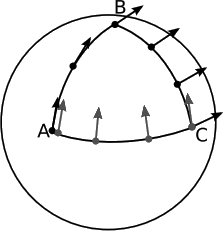
\includegraphics[width = 0.4\textwidth]{figures/parallelTransportSphere.png}
    %\includesvg[width = 0.4\textwidth]{figures/parallelTransportSphere}
    \caption{Parallel Transport on a sphere. Parallel transporting the vector along ABC gives
    a different vector than along AC. Figure from~\cite{parallelTransportFigure}}
    \label{fig:parallelTransportSphere}
\end{figure}

\subsection{Parallelity of Vector Fields}
Let $(\M, \mathcal{O}, \mathcal{A}, \nabla)$ a vector field with connection.
\begin{defn}[Parallel Transport]
    A vector field $X$ on $\M$ is said to be \textit{parallely transported} along a smooth curve $\gamma: \mathbb{R}\to \M$
    if 
    \begin{equation}
        \boxed{
        \nabla_{v_\gamma} X = 0\,.
    }
    \end{equation}
    Another way of writing this is
    \begin{equation}
        \left(\nabla_{v_{\gamma, \gamma(\lambda)}}X\right)_{\gamma(\lambda)}\,,\quad\forall \lambda
    \end{equation}
\end{defn}
\begin{note}
    $v_\gamma$ is not a vector field, but a vector at each point of the curve.
    Here it is actually important that the derivative $\nabla_Y X$ only needs a
    vector field $X$ and a vector $Y$ at the point where the derivative is taken!
\end{note}

\begin{defn}[Parallel]
    A vector $X$ is said to be parallel along the curve $\gamma$ if
    \begin{equation}
        \left( \nabla_{\gamma, \gamma(\lambda)}X  \right)_{\gamma(\lambda)} = \mu(\lambda) X_{\gamma(\lambda)}\,,
    \end{equation}
    for $\mu: \mathbb{R} \to \mathbb{R}$.
    This is a weaker notion than \textit{parallel transported}.
\end{defn}
\textit{Example}: \textit{Euclidean plane} $(\mathbb{R}^2, \mathcal{O}, \mathcal{A}, \nabla_E)$
The red arrows (left picture) are \textit{parallel} along the curve and the blue arrows (right picture)
are \textit{parallel transported} along the curve.
\begin{center}
    \begin{tikzpicture}
        \draw [cyan] plot [smooth, tension=3] coordinates { (0,0) (1,1.5) (2,-2) (3,0)};
        \draw[line width=1pt,blue,-stealth](0,0)--(1,1);
        \draw[line width=1pt,blue,-stealth](-0.09, 1)--(0.91,2);
        \draw[line width=1pt,blue,-stealth](1,1.5)--(2,2.5);
        \draw[line width=1pt,blue,-stealth](2,-2)--(3,-1);
        \draw[line width=1pt,blue,-stealth](3,0)--(4,1);

        \draw [cyan] plot [smooth, tension=3, xshift = -100] coordinates { (0,0) (1,1.5) (2,-2) (3,0)};
        \draw[line width=1pt,red,-stealth, xshift = -100](0,0)--(1,1);
        \draw[line width=1pt,red,-stealth, xshift = -100](-0.09, 1)--(1.91,3);
        \draw[line width=1pt,red,-stealth, xshift = -100](1,1.5)--(1.5,2.0);
        \draw[line width=1pt,red,-stealth, xshift = -100](2,-2)--(3,-1);
        \draw[line width=1pt,red,-stealth, xshift = -100](3,0)--(2,-1);
    \end{tikzpicture}
\end{center}
\begin{note}
    Explanation by Schuller:
    \begin{itemize}
        \item \textit{Parallel transport}: Pinocchio move along the curve and point your nose in the same direction always
            and \textsc{do not lie}.
        \item \textit{Parallel}: Now you're allowed to lie.
    \end{itemize}
\end{note}

\subsection{Autoparallelly Transported Curves}
\begin{defn}[Autoparallelly transported]
    A curve $\gamma: \mathbb{R} \to \M$ is called \textit{autoparallelly transported} (or just \textit{autoparallel}) if
    \begin{equation}
        \nabla_{v_\gamma} v_\gamma = 0\,.
    \end{equation}
    or (this is the same)
    \begin{equation}
        \left( \nabla_{v_{\gamma, \gamma(\lambda)}} v_\gamma \right)_{\gamma(\lambda)} = 0\,.
    \end{equation}
\end{defn}
\begin{note}
    An autoparallel curve is
    \begin{equation}
        \nabla_{v_\gamma} v_\gamma = \mu v_\gamma\,.
    \end{equation}
    even though most of the time one also uses the notion ``autoparallel'' for an autoparallelly transported curve.
    An autoparallelly transported curve is the ``straightest curve possible''.
\end{note}
\textit{Example}: \textit{Euclidean plane} $(\mathbb{R}^2, \mathcal{O}, \mathcal{A}, \nabla_E)$
Red (left): autoparallel curve, blue (right): autoparallelly transported curve.
Equal distances mean equal affine parameter $\lambda$.
\begin{center}
    \begin{tikzpicture}
        \draw[line width=1pt,blue](0,0)--(0.5,0.5);
        \draw[line width=1pt,blue](0.55,0.55)--(1,1);
        \draw[line width=1pt,blue](1.05,1.05)--(1.5,1.5);
        \draw[line width=1pt,blue](1.55,1.55)--(2,2);
        \draw[line width=1pt,blue](2.05,2.05)--(2.5,2.5);
        \draw[line width=1pt,blue](2.55,2.55)--(3.1,3.1);

        \draw[line width=1pt,red,xshift = -100](0,0)--(1,1);
        \draw[line width=1pt,red,xshift = -100](1.05,1.05)--(1.5,1.5);
        \draw[line width=1pt,red,xshift = -100](1.55,1.55)--(1.7,1.7);
        \draw[line width=1pt,red,xshift = -100](1.75,1.75)--(2.5,2.5);
        \draw[line width=1pt,red,xshift = -100](2.55,2.55)--(3.1,3.1);
    \end{tikzpicture}
\end{center}

\subsection{Autoparallel Equation} 
Let $\gamma$ be an autoparallelly transported curve.
Consider that portion of the curve that lies in $U$, where $(U,x)\in \mathcal{A}$ (atlas).
Express $\nabla_{v_\gamma}v_\gamma = 0$ (condition for the curve to be autoparallelly transported)
in terms of chart representatives:
Using $v_{\gamma, \gamma(\lambda)} = \dot{\gamma}^m_{(x)}(\lambda) \left( \frac{\partial}{\partial x^m} \right)_{\gamma(\lambda)}$
and $\gamma^m_{(x)} := x^m \circ \gamma$ we get
\begin{align}
    \nonumber \nabla_{v_\gamma}v_\gamma  &= \left( \nabla_{\dot{\gamma}^m_{(x)} \left( \frac{\partial}{\partial x^m} \right)} \dot{\gamma}^n_{(x)}  \frac{\partial}{\partial x^n}  \right)\\
    &= \underbrace{\dot{\gamma}^m \frac{\partial \dot{\gamma}^q}{\partial x^m}}_{\ddot{\gamma}^m_{(x)}} \frac{\partial}{\partial x^q} + \dot{\gamma}^m \dot{\gamma}^n \Gamma^q{}_{nm}\frac{\partial}{\partial x^q}\,.
    \label{eq:autoparallelEquation}
\end{align}
In summary we have the chart expression of the condition that $\gamma$ be autoparallelly transported:
\begin{equation}
    \boxed{%
    \ddot{\gamma}^{m}_{(x)}(\lambda) + \Gamma^m{}_{ab}(\gamma(\lambda)) \dot{\gamma}^a(\lambda)\dot{\gamma}^b(\lambda) = 0}\,.
\end{equation}
As we will see later if for $\Gamma$ we choose the so called \textit{Levi Civita connection}
then this is the \textit{geodesic equation}.

\paragraph{Examples}
\begin{enumerate}
    \item Euclidean plane:\\ $U = \mathbb{R}^d$, $x = \mathrm{id}_{\mathbb{R}^d}$, $\Gamma_(x)^{i}{}_{jl} = 0$,
        $\Rightarrow \ddot{\gamma}^m_{(x)} = 0$ $\Rightarrow \gamma_{(x)}^m(\lambda) = a^m \lambda + b^m$, $a,b\in \mathbb{R}^d$
    \item Round sphere $(S^2, \mathcal{O}, \mathcal{A}, \nabla_\text{round})$:\\
        The sphere $S^2$ as a manifold does not contain the notion of distances like we are used to from a sphere.
        Also a squished and stretched sphere is still a sphere. 
        Only when we choose a specific connection $\nabla_\text{round}$ we get what we usually see as the sphere,
        but it's actually the \textit{round sphere}.
        Consider a chart (polar coordinates)
        \begin{align}
            \nonumber x(p) &= (\theta, \phi)\,, \\
            \nonumber \theta \in (0, \pi)\,&,\quad \phi \in (0, 2\pi)\,\\
            \Gamma^1_{(x)22} (x^{-1}(\theta, \phi)) &:= - \sin\theta \cos\theta\,,\\
            \Gamma^2_{(x)21} = \Gamma^2_{(x)12} &:= \cot \theta\,.
        \end{align}
        and all other $\Gamma$s zero.
        Using sloppy notation
        \begin{align}
            x^1(p) = \theta{p}\,,
            x^2(p) = \phi(p)\,,
        \end{align}
        the autoparallel equation becomes
        \begin{align}
            \ddot \theta - \sin\theta \cos\theta\, \dot\phi \dot\phi &= 0\,,\\
            \ddot \phi + 2\cot\theta\, \dot\theta \dot\phi &= 0\,.
        \end{align}
        For example a solution is 
        \begin{align}
            \theta(\lambda) &= \pi/2 = \text{const}\,,\\
            \phi(\lambda) &= \omega \lambda + \phi_0\,.
        \end{align}
        This is a curve around the equator with constant speed.
        Similarity other curves along great circles are solutions.
\end{enumerate}
\begin{note}
    Thus if someone gives you the connection $\nabla_\text{potato}$ on a potato,
    you can calculate the straightest curves on that potato.
    Still, the potato is a 2-sphere $S^2$ as a smooth manifold.
\end{note}

\subsection{Torsion}
\begin{defn}[Commutator]
    The commutator between two vector fields $X$ and $Y$ is defined as
    \begin{equation}
        [X,Y]f := X(Y f) - Y(Xf)\,.
    \end{equation}
\end{defn}
\begin{defn}[Torsion]
    The \textit{torsion} of a connection $\nabla$ is the $(1,2)$-tensor field
    \begin{equation}
    T(\omega, X, Y) := \omega \left( \nabla_X Y - \nabla_Y X - [X,Y] \right)\,,
    \end{equation}
\end{defn}
Proof that $T$ is a tensor: Check $T$ is $C^\infty$-linear in each entry
\begin{enumerate}
    \item 
        \begin{equation}
            T(f\omega, X, Y) = f \omega (\ldots) = f T(\omega, X,Y)\,,
        \end{equation}
        \begin{align}
            T&(\omega + \psi, X, Y) = (\omega + \psi) (\ldots)\\
            \nonumber &= T(\omega, X,Y) + T(\psi, X, Y)\,,
        \end{align}
    \item
        \begin{align}
            \nonumber T&(\omega, fX, Y) = \omega \left( \nabla_{fX} Y - \nabla_Y (fX) - [fX, Y] \right)\\
            \nonumber &= \omega \left[ f\nabla_X Y - f \nabla_Y X - \cancel{(Yf)X} - fXY \right.\\
            &~\left.- fYX - \cancel{(Yf)X} \right] = f T(\omega, X, Y)\,,
        \end{align}
        where we have used
        \begin{align}
            [fX,Y]g &= fX(Yg) - Y(fXg) \\
            \nonumber &= fX(Yg) - (Yf)Xg - f(YXg)\,,
        \end{align}
        and $\nabla_Y f = Yf$.
        Since $T(\omega,X,Y) = -T(\omega, Y, X)$ we don't have to check the scaling
        in the last argument and the additivity in the middle argument also is easy.
\end{enumerate}
\begin{defn}[Torsion-free connection]
    $(\M, \mathcal{O}, \mathcal{A}, \nabla)$ is called \textit{torsion-free} if $T=0$.
    In a chart:
    \begin{equation}
        T^i{}_{ab} := T\left(\diff x^i, \frac{\partial}{\partial x^a}, \frac{\partial}{\partial x^b}\right) = 
        2\Gamma^i_{[ab]}\,.
    \end{equation}
\end{defn}
From now on we will be focusing on \textit{torsion-free} connections.

\subsection{Curvature}
\subsubsection{Riemann Curvature Tensor}
\begin{defn}[Riemann Curvature]
    The \textit{Riemann Curvature} of a connection $\nabla$ is the
    (1,3)-tensor field
    \begin{align}
        \nonumber \Riem(\omega, Z, X, Y) := w&\left( \nabla_X \nabla_Y Z - \nabla_Y\nabla_X Z \right.\\
        &-\left. \nabla_{[X,Y]}Z \right)\,.
        \label{eq:RiemannCurvature}
    \end{align}
\end{defn}
\begin{note}
    The Riemmann curvature tensor contains all information about the curvature.
    For a two-dimensional manifold the Ricci tensor is enough.
\end{note}
\begin{note}
    Of course one has to show that $\Riem$ is $C^\infty$-linear in each slot. 
    The first slot is trivial, I will show it for the second:
    \begin{align*}
         &\Riem(\omega, fZ, X, Y) := \\ 
         &=\omega\left( \nabla_X \nabla_Y (fZ) - \nabla_Y\nabla_X (fZ) - \nabla_{[X,Y]}(fZ) \right)\,.\\
         &=\omega\left[ \nabla_X( (Yf)Z) + f\nabla_Y Z) - \right.\\
         &\phantom{=}\left.\nabla_Y( (Xf)Z - f\nabla_X Z) - ([X,Y]f)Z - f\nabla_{[X,Y]}Z\right]\\
         &= \omega\left[ ( (XY - YX) f )Z + f(\nabla_X\nabla_Y - \nabla_Y\nabla_X)Z\right.\\
         &\phantom{=} \left. - ([X,Y]f)Z - f\nabla_{[X,Y]}Z\right]\\
         &= f \Riem(\omega, Z, X, Y)\,.
     \end{align*}
     The third (and by symmetry also forth) argument works the same, one just has to use
     \begin{align}
         \nonumber\nabla_{[fX,Y]}Z &= \nabla_{f[X,Y]Z - (Yf)X}Z  \\
         &=f\nabla_{[X,Y]}Z - (Yf)\nabla_X Z\,.
     \end{align}
\end{note}


\subsubsection{Algebraic Relevance of Riem}
\begin{align}
    \nonumber &\left( \nabla_X \nabla_Y - \nabla_Y \nabla_X \right)Z =\\ %cant have & in \left \right
    &\phantom{blabla}\Riem(\cdot, Z,X,Y) + \nabla_{[X,Y]}Z
\end{align}
Let's look at a chart $(U,x)$.
We write $\nabla_{\frac{\partial}{\partial x^a}} = \nabla_a$, but be careful, because when
writing it like this we throw away the information of the chart in $\nabla$.
\begin{align}
    \boxed{\left( \nabla_a\nabla_b Z \right)^m - (\nabla_b\nabla_a Z)^m = R^m{}_{nab}Z^n
    }
    \\\nonumber+ \cancel{\nabla_{[\frac{\partial}{\partial x^a},\frac{\partial}{\partial x^b}]}Z}\,,
\end{align}
where with $R^{m}{}_{nab}$ we now denote the components of $\Riem$ in the basis.
<<<<<<< HEAD

\subsubsection{Geometric Relevance of Riem}
\begin{center}
    \textsc{Put picture here of $[X,Y] = 0$ and
    $[X,Y] \neq 0$}.
    Schuller did a really god job explaining this at the end of lecture
    8, but it's hard to write down.
\end{center}

Assuming a torsion-free connection, $T=0$, then one can imagine curvature as follows.
Parallel transporting a vector $Z$ along two different paths from $p$ to $q$
changes the vector.
Going infinitesimal and ``along'' $X$ or $Y$ (first along $X$ and then along $Y$ or the other
way round) one can find (for $[X,Y] = 0$)
\begin{equation}
    (\delta Z)^m = R^m{}_{nab}X^aY^bZ^n\,\delta s\delta t\,,
\end{equation}
plus higher order terms in the ``lengths of the curves'' $\delta s$, $\delta t$.
%One contracts the first and the third index, because all others are either zero or equivalent.


\section{Newtonian Spacetime is Curved!?}
Let's review Newton's axioms:
\begin{enumerate}
    \item A body on which \textit{no force} acts moves uniformly along a straight line.
    \item \textit{Deviation} of a body's motion from such uniform straight motion is effected by a
        force, reduced by a factor of the body's reciprocal mass.
\end{enumerate}
One might think that the first axiom is a special case of the second.
The problem with that is that the second axiom needs to know what a 
straight line is.
So it might be a better idea to interpret the first axiom as a measurement prescription
for the geometry of space that tells us what a straight line is.
The second problem is: Gravity acts universally on every particle, so how should
the first axiom ever be applicable if there are at least two particles in the
universe?

Maybe similar reasoning lead Laplace (1749-1827) to state the following question:
\begin{quote}
    Can gravity be encoded in a curvature of space, such that particles that are subject
    to no other force than gravity, move in straight lines in this curved space?
    In other words: Can we get rid of the gravitational ``force'' and put it into the
    geometry of space?\footnote{%
        Not sure if I wrote this correctly. The text in the lecture~\cite{Schuller15}
    is strangely formulated.}
\end{quote}
\paragraph{Answer}: No!
\paragraph{Proof}:
Newton's equation and Laplace's equation are
\begin{align}
    \label{eq:newton} \cancel{m} \ddot{x}^i(t) &= \cancel{m} f^{i}(x(t)) = F^i\,,\\
    -\partial_i f^i &= 4\pi G \rho\,,\\
\end{align}
where $F$ denotes the force, $m$ the mass and $\rho$ the density.
If we could encode this in curvature then we should be able to write equation~(\ref{eq:newton})
as
\begin{align}
    &\ddot{x}^i(t) - f^i(x(t)) = 0\\
    =~&\ddot{x}^i(t) + \Gamma^i_{ab}\dot{x}^a(t)\dot{x}^b(t) = 0
\end{align}
But that is just not possible, since $f^i$ does not depend on the velocity $\dot(x^a)$.

But lo and behold:
We have not used the word \textit{uniformly} in the first axiom.
That basically means that the equal distances are passed in equal times.
\begin{note}
    A curve is more than the set of its points!
    It's the set of its points and its parametrization! 
\end{note}
The trick is: When we have a curve $\gamma(t)$ we can plot it in a coordinate
system with one dimension more that we take as time (just like s-t diagrams in school).
Then we basically put the information of the parametrization in the form of the line
in this space. 

\begin{center}
    \begin{tikzpicture}
        \draw[line width=1pt,blue, xshift = -100](0,0)--(0.5,0.5);
        \draw[line width=1pt,blue, xshift = -100](0.55,0.55)--(1,1);
        \draw[line width=1pt,blue, xshift = -100](1.05,1.05)--(1.5,1.5);
        \draw[line width=1pt,blue, xshift = -100](1.55,1.55)--(2,2);
        \draw[line width=1pt,blue, xshift = -100](2.05,2.05)--(2.5,2.5);
        \draw[line width=1pt,blue, xshift = -100](2.55,2.55)--(3.1,3.1);

        \draw[line width=1pt,red](0,0)--(1,1);
        \draw[line width=1pt,red](1.05,1.05)--(1.8,1.8);
        \draw[line width=1pt,red](1.85,1.85)--(2.4,2.4);
        \draw[line width=1pt,red](2.45,2.45)--(2.8,2.8);
        \draw[line width=1pt,red](2.85,2.85)--(3,3);
    \end{tikzpicture}
    \begin{tikzpicture}
        \draw [<->,thick, xshift = -100] (0,3.2) node (taxis) [above] {$t$}
        |- (3.2,0) node (xaxis) [right] {$x$};

        \draw[line width=1pt,blue, xshift = -100](0,0)--(0.5,0.1);
        \draw[line width=1pt,blue, xshift = -100](0.55,0.12)--(1,0.2);
        \draw[line width=1pt,blue, xshift = -100](1.05,0.22)--(1.5,0.3);
        \draw[line width=1pt,blue, xshift = -100](1.55,0.32)--(2,0.4);
        \draw[line width=1pt,blue, xshift = -100](2.05,0.42)--(2.5,0.5);
        \draw[line width=1pt,blue, xshift = -100](2.55,0.52)--(3.1,0.6);

        \draw [<->,thick, xshift = 20] (0,3.2) node (taxis) [above] {$t$}
        |- (3.2,0) node (xaxis) [right] {$x$};
        \draw[line width=1pt, red, xshift = 20](0,0)--(0.5,0.1);
        \draw[line width=1pt, red, xshift = 20](0.52,0.12)--(1,0.3);
        \draw[line width=1pt, red, xshift = 20](1.02,0.32)--(1.5,0.6);
        \draw[line width=1pt, red, xshift = 20](1.52,0.62)--(2,0.9);
        \draw[line width=1pt, red, xshift = 20](2.02,0.92)--(2.5,1.3);
        \draw[line width=1pt, red, xshift = 20](2.52,1.32)--(3.1,1.8);
        %\draw (0,0) coordinate (a_1) -- (2,1.8) coordinate (a_2);
        %\draw (0,1.5) coordinate (b_1) -- (2.5,0) coordinate (b_2);
        %\coordinate (c) at (intersection of a_1--a_2 and b_1--b_2);
        %\draw[dashed] (yaxis |- c) node[left] {$y'$}
        %-| (xaxis -| c) node[below] {$x'$};
        %\fill[red] (c) circle (2pt);
    \end{tikzpicture}
\end{center}

So now let us try not only in space, but in (Newtonian) spacetime:\\
\bigskip
\begin{minipage}{0.19\textwidth}
Let $x: \mathbb{R} \to \mathbb{R}^3$ be the particle's trajectory
in space fulfilling Newton's law $\ddot{x}^i = f^i(x(t))$.
\end{minipage}
\hfill
$\leftrightarrow$
\hfill
\begin{minipage}{0.25\textwidth}
    worldline (history) of the particle
    $X: \mathbb{R} \to \mathbb{R}^4$\\
    $t\mapsto (t, x^1(t), x^2(t), x^3(t))$
    $:= (X^0(t), X^1(t), X^2(t), X^3(t))$
\end{minipage}
Trivial rewritings:
\begin{equation}
    \dot{X^0} = 1
\end{equation}
and
\begin{align}
    \ddot{X}^0 &= 0\,,\\
    \ddot{X}^i - f^i(X(t))\dot{X}^0\dot{X}^0 &= 0\,,\quad i=1,2,3\,,
\end{align}
which is equivalent to
the autoparallel equation in spacetime
\begin{equation}
    \ddot{X}^\alpha + \Gamma^\alpha{}_{\beta \gamma} \dot{X}^\beta \dot{X}^\gamma = 0\,,\quad \alpha=0,1,2,3\,,
\end{equation}
with
\begin{equation}
    \Gamma^i{}_{00} = -f^i\,,
\end{equation}
and all other components of $\Gamma$ zero.

This is not a coordinate-choice artefact, since
\begin{equation}
    R^{a}{}_{0b0} = -\frac{\partial}{\partial x^b}f^a \neq 0\,\\
\end{equation}
and
\begin{equation}
    R_{00} = R^\mu{}_{0\mu 0} = -\partial f^a = 4\pi G \rho\,.
\end{equation}
If you already know the solution (General Relativity) you can cheat and write
$T_{00} = \rho/2$ to get
\begin{equation}
    R_{00} = 8 \pi G T_{00}\,.
    \label{eq:newtGR}
\end{equation}
Thus Newtonian spacetime is curved (only in time) even if we do not
have relativity and the curvature is prescribed by the distribution of
matter $\rho$.
Uniformly straight in space $\to$ straight in spacetime.

In fact Einstein proposed an equation similar to~(\ref{eq:newtGR}) in 1912, namely
\begin{equation}
    R_{\mu\nu} 8 \pi G T_{\mu\nu}\,,\quad \mu,\nu = 0,1,2,3\,,
\end{equation}
which is not entirely correct, but almost.

\subsection{Foundations of the Geometric Formulation of Newton's Axioms}
\begin{defn}[Newtonian Spacetime]
    A Netwonian spacetime (space+time) is a quintuple
    \begin{equation}
        (\M, \mathcal{O}, \mathcal{A}, \nabla, t)\,,
    \end{equation}
    where $(\M, \mathcal{O}, \mathcal{A})$ form a 4-dimensional smooth manifold and
    the \textit{absolute time}
    \begin{equation}
        t: \M\to\mathbb{R}\,,\quad\text{smooth function}\,,
    \end{equation}
    satisfies
    \begin{enumerate}
        \item There is an absolute space that follows from the existence of absolute time.
            \begin{equation}
                \left( \diff t \right)_p \neq 0\,,\quad\forall p\in\M\,,
            \end{equation}
        \item Absolute time flows uniformly,
            \begin{equation}
                \nabla \diff t = 0\,,\quad\text{everywhere}
            \end{equation}
        \item $\nabla$ is torsion free.
    \end{enumerate}
\end{defn}
\begin{defn}[Absolute space $S_\tau$ at time $\tau$]
    \begin{equation}
        S_\tau:=\left\{ p\in\M | t(p) = \tau \right\}\,,
    \end{equation}
    and thus because of $(\diff \tau)_p \neq 0$
    \begin{equation}
        \M = \bigcupdot S_\tau\,,
    \end{equation}
    where $\bigcupdot$ means the disjoint union.
\end{defn}
This means that $S_\tau$ \textit{foliate} spacetime.
\begin{note}
    By $\nabla \diff t$ we mean that the argument that $\nabla_\cdot$ takes is
    open, so what comes out is a (0,2)-tensor.
\end{note}
\begin{note}
    You can view Gravity as curvature of spacetime and already in Newtonian mechanics
    this is not just an alternative formulation,
    but if you look at the first axiom there is not really another possible choice.
    It's not relativity that forces us to use spacetime, it's gravity itself.
\end{note}
\begin{defn}[]
    A vector $X\in\T{p}\M$ is called
    \begin{enumerate}
        \item future-directed if
            \begin{equation}
                \diff t(X) > 0\,,
            \end{equation}
        \item spatial if
            \begin{equation}
                \diff(X) = 0\,,
            \end{equation}

        \item past-directed if
            \begin{equation}
                \diff{X}<0\,.
            \end{equation}
    \end{enumerate}
\end{defn}
\paragraph{Newton 1:} The worldline of a particle under the influence
of no force (gravity isn't a force now) is a \textit{future directed
autoparallel},\textit{i.e.}\ everywhere
\begin{align}
    \nabla_{v_X}v_X &= 0\,,
    \diff t(v_X)>0\,.
\end{align}
\paragraph{Newton 2:}
The acceleration of a worldline
\begin{equation}
    \underbrace{\nabla_{v_X}v_X}_a = \frac{F}{m}\,,
\end{equation}
where $F$ is a spatial vector field: $\diff t(F) =0$, $X$ is a future directed vector
and $a$ is the acceleration.
\paragraph{Convention:}
Restrict attention to \textit{stratified atlases} $\mathcal{A}_\text{stratified}$
whose charts $(U,x)$ have the property
\begin{equation}
    x^0 = t\eval_U
\end{equation}
In a stratified atlas the first axiom becomes
\begin{align}
    0 = \left( \nabla_\frac{\partial}{\partial x^a} \diff x^0 \right)_b = -\Gamma^0_{ba}\,.
\end{align}

\subsubsection{Geometric Relevance of Riem}
\begin{center}
    \textsc{Put picture here of $[X,Y] = 0$ and
    $[X,Y] \neq 0$}.
    Schuller did a really god job explaining this at the end of lecture
    8, but it's hard to write down.
\end{center}

Assuming a torsion-free connection, $T=0$, then one can imagine curvature as follows.
Parallel transporting a vector $Z$ along two different paths from $p$ to $q$
changes the vector.
Going infinitesimal and ``along'' $X$ or $Y$ (first along $X$ and then along $Y$ or the other
way round) one can find (for $[X,Y] = 0$)
\begin{equation}
    (\delta Z)^m = R^m{}_{nab}X^aY^bZ^n\,\delta s\delta t\,,
\end{equation}
plus higher order terms in the ``lengths of the curves'' $\delta s$, $\delta t$.
One contracts the first and the third index, because all others are either zero or equivalent.

Let's evaluate Newton 2 in a chart $(U,x)$ of a stratified atlas $\mathcal{A}_\text{stratified}$:

\fbox{Finish this section}


\section{Metric Manifolds}
\subsection[The metric g]{The metric $g$}
We establish a new structure called a \textit{metric} on a smooth manifold $\M$
that allows to assign a length to each vector $X$ in each tangent space $X\in
\T_p\M$ and an angle between vectors in the same tangent space.

Since the velocity $v_{\gamma,p}$ of a curve $\gamma$ at the point $p\in\M$
(defined by equation~(\ref{eq:defVelocity})) is a vector, we can then integrate
up the lengths of the velocities to get the length of a curve.

Then we require that the shortest curves are also the straightest curves,
$\nabla_{v_\gamma} v_\gamma=0$, which will result in the metric determining
the connection $\nabla$ if there is no torsion ($T=0$) and thus also the
curvature.

\begin{defn}[Metric]
    A metrig $g$ on a smooth manifold $(\M, \mathcal{O}, \mathcal{A})$ is a
    (0,2)-tensor field satisfying
    \begin{itemize}
        \item \textit{symmetry}:
            \begin{equation}
                g(X,Y) = g(Y,X)\,,\quad\forall X,Y\in\Gamma(\T\M)\,,
            \end{equation}
        \item \textit{non-degeneracy:} There are no non-zero vectors $X\in\T{p}\M$
            with
            \begin{equation}
                g(X,Y) = 0\,\quad \forall Y\in\T_p\M\,.
            \end{equation}

    \end{itemize}
\end{defn}

\begin{defn}[Inverse Metric $g^{-1}$]
    The symmetric (2,0)-tensor field $g^{-1}$ with respect to a metric $g$ is
    \begin{align}
        g^{-1}: \Gamma(\T^*\M) &\times\Gamma(\T^*\M) \linearto C^\infty(\M)\,\\
        (\omega, \sigma) &\mapsto w\left( \flat^{-1}(\sigma) \right)\,.
    \end{align}
\end{defn}

\begin{defn}[Musical map $\flat$]
    The musical map (``flat'')
    \begin{align}
        \label{eq:musicalMap}
        \flat: \Gamma(\T\M) &\to \Gamma(\T^*\M)\,\\ 
        X &\mapsto \flat(X)\,,
    \end{align}
    where
    \begin{equation}
        \flat(X)(Y):= g(X,Y)\,,
    \end{equation}
    \textit{i.e.}\ the musical map is like a partial evaluation
    of the metric, $\flat(X) = g(X,\cdot)$ and can also be written
    with indices and the so called raising and lowering of indices
    \begin{align}
        X_a := g_{am}X^m := \left( \flat(X) \right)_a\,\\
        X^a := g^{am}X_m := \left( \flat^{-1}(X) \right)^a\,
    \end{align}
\end{defn}

\begin{note}
    In a chart $g_{ab} = g_{ba}$ and
    \begin{equation}
        \left( g^{-1} \right)^{am} g_{mb} = \delta^a_b\,,
        \label{eq:inverseMetricComponents}
    \end{equation}
    but the inverse metric is not really an inverse of the metric.
    We see this by looking at the spaces:
    \begin{align}
        g&: \Gamma(\T\M)\times \Gamma(\T\M) \to C^\infty(\M)\,,\\
        g^{-1}&: \Gamma(\T^*\M)\times \Gamma(\T^*\M) \to C^\infty(\M)\,,
    \end{align}
    so it is not really the inverse map, but the inverse matrix in the sense
    of equation~(\ref{eq:inverseMetricComponents}).
\end{note}
\begin{note}
    Pulling down or up indices is a dangerous business.
    It means we are suppressing the metric and hiding
    that the object depends on the metric.
    Actually it then is not clear if $X_a$ are the
    components of a genuine one form or if it is
    constructed by pulling down the index of the index
    of a vector and hiding the metric.
\end{note}

\paragraph{Example: Sphere} $(S^2, \mathcal{O}, \mathcal{A})$
with a chart $(U,x)$, $\phi\in(0,2\pi)$, $\theta\in (0,\pi)$.
\begin{equation}
    g_{ij}\left(x^{-1}(\theta, \phi)\right) = 
    \begin{pmatrix}
        R^2 & 0 \\
        0 & R^2 \sin^2 \theta
    \end{pmatrix}_{ij}\,,
\end{equation}
is the metric of the \textit{round sphere} of radius $R\in\mathbb{R}^+$.

\subsection{Signature}
Remember \textit{linear algebra}:
Eigenvalues and eigenvectors
\begin{equation}
    A^a{}_m v^m = \lambda v^a\,.
    \label{eq:eigenvector}
\end{equation}
How does this translate the notion of eigenvectors to our case of a metric?
$A^a{}_m$ is a (1,1)-tensor and eigenvectors are a good notion,
but for a (0,2)-tensor eq.~(\ref{eq:eigenvector}) does not work
\begin{equation}
    g_{am}v^m \neq \lambda v^a\,.
\end{equation}
\begin{note}
    A (1,1) tensor cannot be symmetric on its own, it can only be symmetric
    with respect to a metric, \textit{i.e.}\ one can pull down an index
    and then switch indices.
\end{note}
\begin{itemize}
    \item A (1,1)-tensor has eigenvalues and can be transformed to look like
        \begin{equation}
            \begin{pmatrix}
                \lambda_1 & & \\
                & \ddots & \\
                & & \lambda_n
            \end{pmatrix} = \diag(\lambda_1, \ldots, \lambda_n)\,,
        \end{equation}
        with eigenvalues $\lambda_i$.
    \item A (0,2)-tensor like the metric has a \textit{signature} $(p,q)$ and can be transformed to
        \begin{equation}
            \diag(\underbrace{1,\dots, 1}_{p}, \underbrace{-1, \ldots, -1}_{q}, 
            \underbrace{0, \ldots, 0}_{\dim V - p - q})\,,
        \end{equation}
        which we can agree has way less information than the eigenvalues.
\end{itemize}
\begin{note}
    The condition that the musical isomorphism $\flat$, eq.~(\ref{eq:musicalMap})
    is invertible means that there are no zeros in the signature. 
    Basically a zero would mean that a whole subspace is mapped to zero and
    this is not invertible.
\end{note}

\begin{defn}[Riemannianian and Lorentzian Metric]
    \begin{itemize}
        \item A metric is called \textit{Riemannian} if its signature is
            $(+, \ldots, +)$ (or $(-, \ldots, -)$ is equivalent).
        \item A metric is called \textit{Lorentzian} if its signature is
            $(+,-, \ldots, -)$ (or $(-,+, \ldots, +)$ is equivalent).
            We will chose $(+,-, \ldots, -)$ here.
            This is what we need for General Relativity.
        \item All other signature including Lorentzian metrics are called
            \textit{pseudo Riemannian}.
    \end{itemize}
\end{defn}
\begin{note}
    One might call a non-Riemannian metric a \textit{pseudo metric}, since
    there are nonzero vectors that have zero length under such a metric.
    In a Lorentzian manifold one says they lie on the light cone.
\end{note}
\begin{note}
    Generally the metric itself will change from point to point in spacetime $\M$,
    but the signature stays.
\end{note}
\subsection{Length of a Curve}
Let $\gamma$ be a smooth curve.
Then we know its velocity $v_{\gamma,\gamma(\lambda)}(f) := (f \circ \gamma)'(\lambda)$
at each $\gamma(\lambda)\in \M$ from definition~\ref{defn:velocity}.

\begin{defn}[Speed of a curve]
    On a \textit{Riemannian metric manifold} $(\M, \mathcal{O}, \mathcal{A}, G)$ the
    \textit{speed} of a curve $\gamma$ at $\gamma(\lambda)$ is the number
    \begin{equation}
        s(\lambda) = \left( \sqrt{g(v_\gamma, v_\gamma)} \right)_{\gamma(\lambda)}\,.
    \end{equation}
    Basically its just the magnitude of the velocity.
\end{defn}
\begin{note}
    I feel the need, the need for \cancel{speed} a metric to define speed.
\end{note}
\begin{note}
    The physical dimensions are
    \begin{align*}
        [v^a] &= \frac{1}{T}\,,\\
        [g_{ab}] &= L^2\,,\\
        [\sqrt{g_{ab}v^av^b}] &= \frac{L}{T}\,.
    \end{align*}
    The idea that coordinate distance has anything to do with real distance is just wrong.
    Going double as far in coordinates has nothing to do with going double as far
    in ``reality'' (the manifold $\M$).
\end{note}

\begin{defn}[Length of a curve]
    Let $\gamma: (0,1)\to \M$ be a smooth curve.
    Then the \textit{length of} $\gamma$ is the number
    \begin{align}
        L[\gamma] &:= \int_0^1 \diff \lambda\, s(\lambda) \\
        &= \int_0^1\diff \lambda\, \sqrt{\left( g(v_\gamma,v_\gamma \right)_{\gamma(\lambda)}}\,.\nonumber
            \label{eq:lengthCurve}
    \end{align}
    It is a functional, \textit{i.e.}\ a function is mapped to a number.
\end{defn}
\begin{note}
    It's exactly the other way than one usually thinks.
    Velocity is more fundamental than speed and speed is more fundamental than
    length.
\end{note}

\paragraph{Example:} The round sphere of radius $R$.
Its equator is a curve
\begin{align}
    \theta(\lambda) &:= (x^1\circ \gamma)(\lambda) = \frac{\pi}{2}\,,\\
    \phi(\lambda) &:= (x^2\circ\gamma)(\lambda) = 2\pi \lambda^3\,,
\end{align}
where we have randomly chosen any parametrization that has
$\phi(0) = 0$, $\phi(1) = 2\pi$.
Then the components of the velocity are (eq.~(\ref{eq:vectorcomponents2}))
\begin{align*}
    v^i &= \dot{\gamma}_x^i (0) := (x^i\circ\gamma)'(0)\,,\\
    v^1 &= \left( \frac{\pi}{2} \right)' = 0\,,\\
    v^2 &= \left( 2\pi \lambda^3 \right)' = 6\pi \lambda^2\,.
\end{align*}
and $g_{ij} = \diag(R^2, R^2 \sin^2\theta)$ the length of the curve around the equator
($\theta = \pi/2$, $\sin(\theta) = 1$)
\begin{align*}
    L[\gamma] &= \int_0^1\diff\lambda\,\sqrt{R^2\cdot 0 + R^2 \sin^2(\theta(\lambda))(6\pi\lambda^2)^2}\\
    &= \int_0^1\diff\lambda\, R 6 \pi \lambda^2 = 2\pi R\,,
\end{align*}
or just to have it written down in a rigorous way
\begin{align*}
    &L[\gamma] =\\
    &\int_0^1\diff\lambda\,\sqrt{g_{ij}(x^{-1}(\theta(\lambda),\phi(\lambda))(x^i\circ\gamma)'(\lambda)
        (x^j\circ\gamma)'(\lambda)}
\end{align*}

\begin{theorem}[Reparametrization invariance of the lengh of a curve]
    Let $\gamma: (0,1)\to\M$ be a curve and
    $\sigma: (0,1)\to(0,1)$ a smooth bijection and increasing (don't drive back
    on the curve), then the reparametrized curve has the same length,
    \begin{equation}
        L[\lambda] = L[\gamma\circ\sigma]\,.
    \end{equation}
\end{theorem}

\subsection{Geodesics}
\begin{defn}[Geodesic]
    A curve $\gamma: (0,1) \to \M$ is called a \textit{geodesic} on a
    Riemannian manifold $(\M, \mathcal{O}, \mathcal{A}, g)$ is a \textit{stationary}
    curve with respect to the length functional $L[\gamma]$.
\end{defn}

\begin{theorem}
    A curve $\gamma$ is a \textit{geodesic} iff it satisfies the Euler-Lagrange equations for
    the Lagrangian
    \begin{align}
        \calL: \T \M &\to \mathbb{R}\,,\\
        X &\mapsto \sqrt{g(X,X)}\,.
    \end{align}
    In a chart the Euler-Lagrange equations take the form (chart dependent)
    \begin{equation}
        \frac{\diff}{\diff \lambda}\left( \frac{\partial \calL}{\partial \dot{\gamma}^m} \right) -
        \frac{\partial \calL}{\partial \gamma^m} = 0\,,
        \label{eq:EulerLagrange}
    \end{equation}
    where
    \begin{equation}
        \calL(\gamma^i, \dot{\gamma}^i) = \sqrt{g_{ij}(\gamma (\lambda)) \dot{\gamma}^i(\lambda)
            \dot{\gamma}^j(\lambda)}\,.
            \label{eq:lagrangian}
    \end{equation}
\end{theorem}
Plugging the Lagrangian~(\ref{eq:lagrangian}) into the Euler-Lagrange equations~(\ref{eq:EulerLagrange})
and using the parametrization of $\gamma$ such that $g(\dot\gamma, \dot\gamma)=1$
(always driving at unit speed) we get after raising the index with $(g^{-1})^{qm}$
\begin{align}
    \ddot{\gamma}^q + 
    \overbrace{\frac{1}{2}\left( g^{-1} \right)^{qm} \left( \partial_i g_{mj} + \partial_j g_{mi}
    - \partial_m g_{ij} \right)}^{:= ^\text{L.C.}\Gamma^q{}_{ij}(\gamma(\lambda))} \dot{\gamma}^i \dot{\gamma}^j = 0\,.
    \label{eq:geodesic}
\end{align}
Equation~(\ref{eq:geodesic}) is the \textit{geodesic equation} for $\gamma$.
We call $^\text{L.C.}\Gamma^q{}_{ij}$ the \textit{Levi-Civita connection coefficient functions}.
\begin{defn}[Levi-Civita connection]
    The \textit{Levi-Civita connection} coefficient functions $^\text{L.C.}\Gamma^q{}_{ij}(\gamma(\lambda))$
    (also called \textit{Christoffel symbols} or ``Christ awful symbols'' because of the labour needed 
    to calculate them)
    of the so called \textit{Levi-Civita connection} $^\text{L.C.}\nabla$ and they are
    \begin{equation}
        \boxed{%
        ^\text{L.C.}\Gamma^q{}_{ij} = 
        \frac{1}{2}\left( g^{-1} \right)^{qm} \left( \partial_i g_{mj} + \partial_j g_{mi}
        - \partial_m g_{ij} \right)
    }
    \end{equation}
\end{defn}
\begin{note}
    If we use the Levi-Civita connection as the connection on our manifold,
    then the geodesic equation
    \begin{equation}
        \ddot{\gamma}^q + \Gamma^q{}_{ij}\dot{\gamma}^i \dot{\gamma}^j = 0\,,
    \end{equation}
    is exactly the equation~(\ref{eq:autoparallelEquation}) for an autoparallelly transported curve,
    \textit{i.e.}\ for a curve that is as straight as possible.
    Choice of the connection as Christoffel conection thus means we identify autoparallelly transported
    curves (straight as possible) with the shortest curves.
\end{note}
\begin{note}
    Thus a metric manifold $(\M, \calO, \calA, g)$ implies a manifold with the Christoffel connection
    \begin{equation}
        (\M, \calO, \calA, g) \to (\M, \calO, \calA, g,~^\text{L.C.}\nabla)\,,
    \end{equation}
    and we usually make this choice of connection.
\end{note}
\begin{note}
    If for a metric manifold $(\M, \calO, \calA, g)$ one imposes
    \begin{enumerate}
        \item \textit{Metric compatibility:} $\nabla g = 0$,
        \item \textit{Absence of torsion:} $T=0$,
    \end{enumerate}
    then the connection is already fixed to be the Levi Civita connection
    $\nabla = {}^\text{L.C.}\nabla$.
    This is the way many General Relativity textbooks go.
    They impose metric compatibility and write the equation $\nabla_i g_{ab}$ in
    three permutations, add them in some way and find an expression for $\nabla$.
    Sadly they usually don't talk about implicitly identifying autoparallelly transported
    curves with the shortest curves by doing this.
\end{note}
\begin{defn}[Riemann-Christoffel Curvature]
    The \textit{Riemann-Christoffel Curvature} $R_{abcd}$ of a manifold
    $(\M, \calO, \calA, g)$ is defined by (in coordinates)
    \begin{equation}
        R_{abcd} := g_{am} R^{m}{}_{bcd}\,,
    \end{equation}
where the connection used to calculate the Riemann tensor $R^m{}_{bcd}$ is the Levi-Civita connection.
\end{defn}
\begin{note}
    In contrast to the Riemann curvature~(\ref{eq:RiemannCurvature}), 
    which only needs a connection, the Riemann-Christoffel cuvature also needs a metric.
\end{note}
\begin{defn}[Ricci Tensor]
    The \textit{Ricci tensor} $R_{ab}$ is defined by (in coordinates)
    \begin{equation}
        R_{ab} := R^m{}_{amb}\,,
    \end{equation}
    where again for the connection to calculate $R^c{}_{amb}$ the Levi-Civita connection is used.
\end{defn}
\begin{defn}[Ricci Scalar Curvature]
    The \textit{Ricci scalar curvature} is
    \begin{equation}
        R := g^{ab}R_{ab}\,,
    \end{equation}
    where we have introduced the \textit{convention}
    \begin{equation}
        g^{ab} := (g^{-1})^{ab} \,.
    \end{equation}
\end{defn}
\begin{defn}[Einstein Curvature]
    The \textit{Einstein Curvature} $G_{ab}$ is defined by
    \begin{equation}
        G_{ab} := R_{ab} - \frac{1}{2} g_{ab} R\,.
    \end{equation}
\end{defn}


\section{Symmetry}
We have the feeling that the \textit{round sphere}
\begin{equation}
    (S^2, \calO, \calA, g^{\text{round}})
\end{equation}
has rotational symmetry, while the potato
\begin{equation}
    (S^2, \calO, \calA, g^{\text{potato}})
\end{equation}
does not.

\subsection{Push-Forward}
\begin{defn}[Push-forward map]
    Let $\mathcal{N}$ and $\M$ be smooth manifolds.
    Let $\phi$ be a map $\phi: \M \to \mathcal{N}$.
    Then the \textit{push-forward} $\phi_*$ is the map
    \begin{equation}
        X \mapsto \phi_*(X)\,,
    \end{equation}
    where $\forall f \in C^\infty(\mathcal{N})$ and $X\in \T\M$
    \begin{equation}
        \phi_*(X)f:= X(f\circ \phi)\,.
    \end{equation}
\end{defn}
\begin{center}
\begin{tikzpicture}
\matrix (m) [matrix of math nodes,row sep=3em,column sep=4em,minimum width=2em]
{%
    \T\M & \T\mathcal{N} & \\
    \M & \mathcal{N} & \mathbb{R}\\
};
\path[-stealth]
(m-1-1) edge node [above] {$\phi_*$} (m-1-2)
(m-1-1) edge node [right] {$\pi_{\T\M}$} (m-2-1)
(m-1-2) edge node [right] {$\pi_{\T\mathcal{N}}$} (m-2-2)
(m-2-1) edge node [above] {$\phi$} (m-2-2)
(m-2-2) edge node [above] {$f$} (m-2-3);
\end{tikzpicture}
\end{center}
\begin{center}
\fbox{\parbox{0.42\textwidth}{%
        \centering
        Vectors are pushed forward.
    }
}
\end{center}
\begin{note}
    Not much happens in the push forward.
    Take a vector $X$ on $\M$ and the push-forward gives a vector on $\mathcal{M}$
    that has the same effect on a function $f$ as $X$ would have on $(f\circ\phi)$.
    One can also take the push-forward of a whole fiber and then
    \begin{equation}
        \phi_*(\T_p\M) \subseteq T_{\phi(p)}\mathcal{N}\,,
    \end{equation}
\end{note}
\paragraph{Components} $\phi_*^a{}_i$ of $\phi_*$ wrt.\ two charts
$(U,x)\in\calA_\M$ and $(V,y)\in\calA_{\mathcal{N}}$,
where $i=1,\ldots,\dim\M$ and $a=1,\ldots,\dim\mathcal{N}$.
\begin{center}
\begin{tikzpicture}
\matrix (m) [matrix of math nodes,row sep=3em,column sep=4em,minimum width=2em]
{%
    M\supset U & V\supset \mathcal{N} \\
    x(U) & y(U)\\
    %\T\M & \T\mathcal{N} & \\
    %\M & \mathcal{N} & \mathbb{R}\\
};
\path[-stealth]
(m-1-1) edge node [above] {$\phi$} (m-1-2)
(m-1-1) edge node [right] {$x$} (m-2-1)
(m-1-2) edge node [right] {$y$} (m-2-2)
(m-2-1) edge node [below] {$y\circ\phi\circ x^{-1}$} (m-2-2)
(m-1-1) edge node [above] {$\hat{\phi}$} (m-2-2);
\end{tikzpicture}
\end{center}
Remember the definition $\diff g (X) = X(g)$ in equation~(\ref{eq:differential}),
then
\begin{align}
    \nonumber \phi_*^a{}_i &= \diff y^a \left( \phi_* \left( \frac{\partial}{\partial^i} \right)_p \right)\\
    \label{eq:pushForwardComponents} &= \phi_*\left( \frac{\partial}{\partial x^i} \right)_p y^a\\
    \nonumber &= \left( \frac{\partial}{\partial x^i} \right)_p \left( y\circ\phi \right)^a
    = \left( \frac{\partial \hat{\phi}^a}{\partial x^i} \right)_p\,.
\end{align}
\begin{note}
    To better understand the push-forward take a smooth curve $\gamma: \mathbb{R} \to \M$ 
    with a tangent vector $v_{\gamma, p}: C^\infty(\M) \linearto \mathbb{R}$.
    Then with $\phi$ one can map the whole curve to $\mathcal{N}$.
    So what happens to the curve $\gamma$ is described by the map $\phi$ and what happens to
    the tangent vector $v_{\gamma, p}$ is  described by the \textit{push-forward}
    $\phi_*$,
    \begin{equation}
        \phi_*(v_{\gamma, p}li) = v_{\phi\circ\gamma, \phi(p)}\,.
    \end{equation}
    \begin{center}
        \fbox{\parbox{0.42\textwidth}{%
                \centering
                The push-forward pushes tangent vectors of curves forward to
                tangent vectors of the mapped (pushed forward) curves.
            }
        }
    \end{center}
\end{note}
\begin{proof}
    Let $\gamma(\lambda_0) = p$, then $\forall f\in C^\infty(\mathcal{N})$
    \begin{align}
        \nonumber \phi_*(v_{\gamma,p})f &= v_{\gamma, p}(f\circ \phi)\\
        \nonumber &= \left( (f\circ\phi)\circ\gamma \right)'(\lambda_0)\\
        \nonumber &= \left( f\circ(\phi\circ\gamma) \right)'(\lambda_0)\\
        &= v_{\phi\circ\gamma,\phi(p)}f\,.
    \end{align}
\end{proof}
\begin{note}
    If $\dim\M < \dim\mathcal{N}$ then $\phi$ is (or can be?) an embedding.
    Then $\phi_*$ converts intrinsic tangent vectors in $\M$ to extrinsic
    tangent vectors in $\mathcal{N}$, just like we often imagine tangent vectors
    to come out of the manifold into a higher space.
\end{note}

\subsection{Pull-Back}
\begin{defn}[Pull-back]
    Let $\phi: \M\to\mathcal{N}$ be a smooth map between two manifolds
    $\M$ and $\mathcal{N}$.
    Then the \textit{pull-back} $\phi^*$ of $\phi$ is
    \begin{align}
        \phi^*: \T^*\mathcal{N} &\to \T^*\M\\
        \omega &\mapsto \phi^*(\omega),
    \end{align}
    where 
    \begin{equation}
        \phi^*(\omega)(X) := \omega\left( \phi_*(X) \right)\,,
    \end{equation}
    for $\omega\in\T^*\mathcal{N}$ and $X\in\T\M$.
    So a form $\omega$ is pulled back, $\phi_*(\omega)$, such that its action on
    a vector $X$ is the same as the action of $\omega$ on the pushed forward
    vector $\phi_*(X)$ on $\omega$.
    \begin{center}
        \fbox{\parbox{0.42\textwidth}{%
                \centering
                Forms are pulled-back.
            }
        }
    \end{center}
\end{defn}
\paragraph{Components} of the pull-back wrt.\ charts are the same as for the pull-back,
which can be seen by just plugging in definitions of the pull-back, differential $\diff y$
and the push-forward,
\begin{align}
    \phi^{*a}_i &:= \phi^*\left( (\diff y^a)_{\phi(p)} \right)\left( \left( \frac{\partial}{\partial x^i} \right)_p \right)\\
    &= \cdots = \phi_*^a{}_i\,.
\end{align}
\begin{itemize}
    \item push-forward:
        \begin{equation}
            \left( \phi_*(X) \right)^a := \phi_*^a{}_i X^i\,,
        \end{equation}
    \item pull-back:
        \begin{equation}
            \left( \phi^*(\omega) \right)_i := \phi^{*a}_i \omega_a\,.
        \end{equation}
\end{itemize}
\begin{note}
    The picture is that if we have a function $f: \mathbb{R}\to \mathcal{N}$
    and take its gradient $\diff f$, we can pull back the gradient to $\M$,
    which should be the same as taking the gradient after ``pulling back''
    the function $f$ with $\phi$:
    \begin{equation}
        \phi^*(\diff f) = \diff (f\circ \phi)\,.
    \end{equation}
\end{note}
\begin{center}
    \begin{tikzpicture}[framed]
\matrix (m) [matrix of math nodes,row sep=3em,column sep=4em,minimum width=2em]
{%
    \T\M & \T\mathcal{N}\\
    \T^*\M & \T^*\mathcal{N}\\
};
\path[-stealth]
(m-1-1) edge node [above] {$\phi_*$} node [below] {push-forward} (m-1-2)
(m-2-2) edge node [above] {$\phi^*$} node [below] {pull-back} (m-2-1);
\end{tikzpicture}
\end{center}

\begin{note}
    If $\phi$ is invertible of course one can also pull back a vector
    by pushing it forward with the inverse map, same for covectors/forms. 
\end{note}

\subsection{Induced Metric}
An important application of the pull-back is when we have an embedding
of one manifold $\M$ in another, higher dimensional one, $\mathcal{N}$,
\begin{equation}
    \M \xhookrightarrow[\text{injective}]{\phi} \mathcal{N}\,,
\end{equation}
From the metric $g$ on $\mathcal{N}$ and the inclusion map $\phi$ we can calculate
the \textit{induced metric} $g_\M$.
For $X,Y\in\T_p \M$
\begin{align}
    g_\M(X,Y) &:= g\left( \phi_*(X), \phi_*(Y) \right)\,,\\
    \left( g_\M \right)_{ij,p} &= (g_{ab})_{\phi(p)}\left( \frac{\partial \hat{\phi}^a}{\partial x^i} \right)_{\phi(p)}
    \left( \frac{\partial \hat{\phi}^b}{\partial x^j} \right)_{\phi(p)}\,.
\end{align}
where again $\hat{\phi}^a = (y\circ\phi)^a$ like in equation~(\ref{eq:pushForwardComponents}).
\begin{note}
    This way we can for example get the induced metric of a 2-sphere $S^2$ in
    $\mathbb{R}^3$.
    This apparently is done in the tutorials of~\cite{Schuller15} and I should do it!
\end{note}
\begin{note}
    Think of $\M=S^2$ embedded in $\mathcal{N} = \mathbb{R}^3$.
    The length of a curve $\gamma$ is defined by eq.~(\ref{eq:lengthCurve}), 
    so basically by the tangent vectors.
    Now one can map the whole curve to $\mathcal{N}$ with $\phi$.
    That means the tangent vectors of $\gamma$ in $\mathcal{N}$ are the 
    pushed forward tangent vectors from $\M$.
    I think we basically require that the lenghts of both curves are the same.
\end{note}

\section{Flow of a Complete Vector Field}
Let $(\M, \calO, \calA)$ be a smooth manifold and $X$ be a vector field on $\M$. 
\begin{defn}[Integral Curve of a Vector Field]
    A curve $\gamma: \mathbb{R} \supseteq I \to \M$ is called an \textit{integral curve}
    of $X$ if
    \begin{equation}
        v_{\gamma, \gamma(\lambda)} = X_{\gamma(\lambda)}\,,
    \end{equation}
    \textit{i.e.}\ at every point the tangent vector of the curve is the vector of the
    vector field at that point, see figure~\ref{fig:integralCurve}.
\end{defn}
\begin{figure}[tbh]
    \centering
    \begin{tikzpicture}
        \begin{axis}[
                width=0.6\textwidth,
                view={0}{90},
                domain=0:2*pi+0.5,
                y domain=0:2*pi+0.5,
                xmax=2*pi+1, ymax=2*pi+1,
                samples=20,
                axis equal image,
                %axis lines = center,
                xtick = {0,3.14,6.28},
                ytick = {0,3.14,6.28},
                xticklabels = {},
                yticklabels = {}
            ]
            \addplot3 [blue, quiver={u={1}, v={sin(deg(x))^2}, scale arrows=0.3, every arrow/.append style={-latex}}] {x};
            \addplot [thick, red] {2-sin(deg(x))*cos(deg(x))/2+x/2};
        \end{axis}
\end{tikzpicture}
    \caption{One integral curve of a vector field.
    Plot adapted from~\cite{texstackexchange:integralCurve}}
    \label{fig:integralCurve}
\end{figure}
\begin{note}
    Think of $X$ as the velocity of water molecules in a river and $\gamma$
    the trajectory of a paper ship that you throw into that river.
\end{note}
\begin{defn}[Complete Vector Field]
    A vector field $X$ is said to be \textit{complete} if all integral curves have
    $I=\mathbb{R}$.
\end{defn}
\begin{note}
    You cannot just reparametrize the curve with something like an arctan, because
    then it is no longer an integral curve!
\end{note}
\begin{theorem}[]
    A compactly supported smooth vector field is complete.
    (Compact: Any open cover a finite subcover, we don't have to understand this at
    the current point.)
\end{theorem}
\begin{defn}[Flow of a Vector Field]
    The \textit{flow of a vector field} $X$ is a one-parameter family
    \begin{align}
        h^X: \mathbb{R}\times\M &\to \M\,,\\
        (\lambda, p) &\mapsto \gamma_p(\lambda)\,,
    \end{align}
    where $\gamma_p:\mathbb{R}\to\M$ is the integral curve of $X$ with
    $\gamma(0) = p$.
\end{defn}
\begin{note}
    For a fixed $\lambda\in\mathbb{R}$
    \begin{equation}
        h^X_\lambda: \M \to \M, \quad\text{smooth}\,,
    \end{equation}
    it takes points of the manifold and pushes them further along the 
    curve~$\gamma$ a parameter distance $\lambda$.
    The same can be done for a set $S\in\M$ and in general
    \begin{equation}
        h^X_\lambda(S) \neq S\,,\quad(\text{if }X\neq 0)\,.
    \end{equation}
\end{note}

\subsection[Lie Subalgebras of the Lie Algabra of Vector Fields]{Lie Subalgebras of the
    Lie Algabra $(\Gamma(\T \M, [\cdot,\cdot])$ of Vector Fields}
    \paragraph{Lie algebra:}
    \begin{equation}
        \Gamma(\T\M) = \{\text{set of all vector fields}\}
    \end{equation}
    is a $C^\infty(\M)$-module.
    We can also restrict ourselfs to the $\mathbb{R}$-vector space,
    \textit{i.e.}\ only multiplication by numbers, not functions.
    Then the \textit{Lie bracket} is $[X,Y]\in\Gamma(\T\M)$, where again
    \begin{equation}
        [X,Y]f := X(Yf) - Y(Xf)\,,
    \end{equation}
    with properties
    \begin{enumerate}
        \item $[X,Y] = - [Y,X]$\,,
        \item $[\lambda X + Z, Y] = \lambda[X,Y] + [Z, Y]$\,,
        \item $[X,[Y,Z]] + [Z,[X,Y]] + [Y, [Z,X]] = 0$ (Jacobi identity).
    \end{enumerate}
    Every structure that fulfills above items and so especially
    $(\Gamma(\T\M), [\cdot,\cdot])$ is called a \textit{Lie algebra}.

    \paragraph{Lie subalgebra:}
    Let $X_1, \ldots, X_s$ be $s$ many vector fields on $\M$, such that
    \begin{equation}
        [X_i, X_j] \ C^k{}_{ij} X_k\,,\quad\forall i,j=1,\ldots,s\,,
        \label{eq:lieSubalgebra}
    \end{equation}
    with the \textit{structure constants} $C^k{}_{ij}\in\mathbb{R}$.
    Then
    \begin{defn}[Lie subalgebra]
        \begin{equation}
            (\mathrm{span}_\mathbb{R}\left\{ X_1,\ldots,X_s \right\}, [\cdot,\cdot])\,,
        \end{equation}
        with eq.~(\ref{eq:lieSubalgebra}) is called a \textit{Lie subalgebra}.
    \end{defn}
    Example on $S^2$:
    \begin{align*}
        [X_1, X_2] = X_3\,,
        [X_2, X_3] = X_1\,,
        [X_3, X_1] = X_2\,,
    \end{align*}
    $(\mathrm{span}_\mathbb{R}\left\{ X_1,\ldots,X_s \right\}, [\cdot,\cdot])=so(3)$.
    Note that we did not need any metric, only a smooth manifold $(S^2, \mathcal{O}_\text{sd}, \calA)$ was needed.
    The vectors are given in a chart $(\theta, \phi)$ by
    \begin{align*}
        X_1(p) &=  -\sin\left( \phi(p) \right)\frac{\partial}{\partial \theta} -
        \cot\left( \theta(p) \right) \cos\left( \phi(p) \right)\frac{\partial}{\partial \phi}\,,\\
        X_2(p) &= \cos\left( \phi(p) \right)\frac{\partial}{\partial \theta} - 
        \cot\left( \theta(p) \sin\left( \phi(p) \right) \right)\frac{\partial}{\partial \phi}\,,\\
        X_3(p) &= \frac{\partial}{\partial \phi}\,.
    \end{align*}

    \subsection{Symmetry}
    \begin{defn}[Symmetry of a Metric]
        An $s$-dimensional Lie subalgebra $(L, [\cdot,\cdot])$ is said to be a
        \textit{symmetry} of asymmetry metric tensor field $g$ if
        $\forall X\in L$ (vector field), $\forall A,B \in \T_p\M$,
        $\forall \lambda \in \mathbb{R}$:
        \begin{equation}
            g\left( (h^X_\lambda)_* (A), (h^X_\lambda)_*(B) \right) = g(A,B)\,,
        \end{equation}
        or put differently:
        \begin{equation}
            (h^X_\lambda)^* g = g\,.
        \end{equation}
    \end{defn}

    \subsection{Lie Derivative}
    If $\forall X \in L$ the \textit{Lie derivative} of the metric
    \begin{equation}
        \mathcal{L}_X g:= \lim_{\lambda \to 0}
        \frac{(h^X_\lambda)^* g - g}{\lambda} =0\,,
    \end{equation}
    then $L$ is a symmetry of $g$.

    \begin{defn}[The Lie Derivative $\mathcal{L}$]
        On a smooth manifold $(\M, \calO,\calA)$, the \textit{Lie derivative}
        $\mathcal{L}$ sends a pair of a \textit{vector field} $X$ and a
        $(p,q)$-\textit{tensor field} $T$ to a $(p,q)$-tensor field 
        $\mathcal{L}_X T$ such that
        \begin{enumerate}
            \item $\Lie_X f = X f$\,, $f\in C^\infty(\M)$\,,
            \item $\left(\Lie_X Yp\right)_p = [X,Y]_p$\,, $Y\in \Gamma(\T\M)$\,,
            \item $\Lie_X(T+S) = \Lie_X T + \Lie_X S$\,,
            \item $\Lie_X\left(T(\omega, Y)\right) = (\Lie_X T) (\omega, Y) +
                T\left( \Lie_X \omega, Y \right) + T(\omega, \Lie_X Y)$\,,
            \item $\Lie_{X+Y}T = \Lie_X T + \Lie_Y T$\,.
        \end{enumerate}
    \end{defn}

    It is a good exercise to calculate the components of the Lie derivative in a chart:
    \begin{align*}
        (&\Lie_X Y)^i = \diff x^i [XY - YX] \\
        &= \diff x^i \left[ X^m \frac{\partial}{\partial x^m}Y^n \frac{\partial}{\partial x^n}
        - Y^n\frac{\partial}{\partial x^n} X^m \frac{\partial}{\partial x^m}\right]\\
        &= \diff x^i \left[ X^m \left( \frac{\partial}{\partial x^m} Y^n \right) \frac{\partial}{\partial x^n}
        - Y^n \left( \frac{\partial}{\partial x^n} X^m \right)\frac{\partial}{\partial x^n}\right]\\
        &= X^m\frac{\partial}{\partial x^m}Y^i - Y^m \frac{\partial}{\partial x^m}X^i\,,
    \end{align*}
    where we have used the product rule for derivatives and that the second derivatives commute.
    Summary:
    \begin{align}
        \left( \Lie_X Y \right)^i &= X^m\frac{\partial}{\partial x^m}Y^i - Y^m \frac{\partial}{\partial x^m}X^i\,,\\
        \left( \nabla_X Y \right)^i &= X^m\frac{\partial}{\partial x^m}Y^i + \Gamma^i{}_{ab}X^a Y^b\,,
    \end{align}
    and in general for the Lie derivative every index up comes with a ``-'' and every index down
    comes with a ``+''.
    \begin{equation}
        \boxed{%
         \left( \Lie_X T \right)^i_j = X^m \frac{\partial}{\partial x^m}\left( T^i_j \right) -
        \frac{\partial X^i}{\partial x^m}T^m_j
        + \frac{\partial X^m}{\partial x^j}T^i_m
    }
    \end{equation}
    \begin{center}
        \fbox{\parbox{0.42\textwidth}{%
                $\nabla_X$: index up comes with $+\Gamma$, index down with $-\Gamma$.\\
                $\Lie_X$: index up comes with $-Y^s \partial/\partial x^s$, index down with +.
            }
        }
    \end{center}
    \begin{note}
        The \textit{connection} $\nabla_X$ is $C^\infty(\M)$-linear in $X$,
        whereas the \textit{Lie derivative} $\Lie_X$ is not, it is just $\mathbb{R}$-linear.
        Also we only have to give a vector $X$ to $\nabla_X$ in order to take the \textit{derivative}
        of a tensor field.
        On the other side $\Lie_X$ needs a vector field $X$.
        For $\nabla_X$ we had to introduce a new structure, the $\Gamma$s, the Lie derivative $\Lie_X$
        needs no new structure.
    \end{note}
    \begin{note}
        Use
        \begin{equation}
            0 = \left( \Lie_X g \right)_{ij} = \ldots
        \end{equation}
        to check whether a metric features a symmetry.
    \end{note}


\section{Integration on Manifolds}
Now we do the completion of our ``lift'' of analysis on the charts to the manifold level.
We want to define
\begin{equation}
    \int_\M f\,,
\end{equation}
and this requires a mild new structure called the \textit{volume form}
and we need to restrict the atlas a little bit (``orientation'').

\subsection[Review of Integration]{Review of Integration on $\mathbb{R}^d$}
\begin{enumerate}
    \item A function $F: \mathbb{R} \to \mathbb{R}$. Assume a notion of integration is known
        (Riemann, Lebesque):
        \begin{equation}
            \int_{(a,b)}F := \int_a^b \diff x\, F(x)\,.
        \end{equation}
    \item $F: \mathbb{R}^d \to \mathbb{R}$.
        On a box-shaped domain
        $I = (a,b)\times(c,d)\times\cdots\times (u,v) \subseteq \mathbb{R}^d$,
        \begin{equation}
            \int_{I} \difff^d\! x\, F(x) := \int_{(a,b)}\diff x^1 \cdots \int_{(u,v)}\diff x^d\,.
        \end{equation}
    \item Other domains $G\subseteq \mathbb{R}^d$:
        \begin{defn}[Indicator function]
            \begin{align}
                \nonumber \mu_G: \mathbb{R}^d &\to \mathbb{R}\,,\\
                x&\mapsto
                \begin{cases}
                    1\,, & \text{if } x\in G\\
                    0\,, & \text{if } x\not\in G
                \end{cases}
            \end{align}
        \end{defn}
        and then define
        \begin{equation}
            \int_G \difff^d\! x F(x):= \int_{-\infty}^\infty \diff x^1 \cdots \int_{-\infty}^\infty \diff x^d \mu_G(x) F(x)\,,
        \end{equation}
        if it exists.
\end{enumerate}
\paragraph{Change of variables}
\begin{center}
    \begin{tikzpicture}
        \matrix (m) [matrix of math nodes,row sep=3em,column sep=4em,minimum width=2em]
        {%
            \mathbb{R}^d \supseteq \mathrm{preim}_\phi(G) & G \subseteq \mathbb{R}^d \\
            ~ & \mathbb{R}\\
        };
        \path[-stealth]
        (m-1-1) edge node [above] {$\phi$} (m-1-2)
        (m-1-2) edge node [right] {$F$} (m-2-2)
        (m-1-1) edge node [below] {$F\circ \phi$} (m-2-2);
            %(m-1-1) edge node [above] {$\phi_*$} node [below] {push-forward} (m-1-2)
            %(m-2-2) edge node [above] {$\phi^*$} node [below] {pull-back} (m-2-1);
    \end{tikzpicture}
\end{center}
\begin{equation}
    \int_G \difff^d\! x\, F(x) = \int\limits_{\mathclap{\mathrm{preim}_\phi(G)}}\difff^d y
    \left|\det(\partial_\cdot \phi^\cdot)(y) \right| (F\circ \phi)(y)\,.
\end{equation}

\subsection{Integration on a Chart}
Let $(\M, \calO, \calA)$ be a smooth manifold and $f: M\to\mathbb{R}$.
Choose two charts $(U,x)\in \calA \ni (U,y)$.
\begin{center}
    \begin{tikzpicture}
        \matrix (m) [matrix of math nodes,row sep=3em,column sep=4em,minimum width=2em]
        {%
            y(u)\subseteq \mathbb{R}^d & \\
            U & \mathbb{R} \\
            x(U) & \\
        };
        \path[-stealth]
        (m-1-1) edge node [above, rotate=-32, scale=0.7] {$f_{(y)}:=f\circ y^{-1}$} (m-2-2)
        (m-2-1) edge node [right] {$y$} (m-1-1)
        (m-2-1) edge node [right] {$x$} (m-3-1)
        (m-2-1) edge node [above] {$f$} (m-2-2)
        (m-3-1) edge node [below, rotate=32, scale=0.7] {$f_{(x)}:=f\circ x^{-1}$} (m-2-2)
        (m-3-1) edge[bend left = 60] node [sloped, above, rotate=180, pos=0.5] {$\phi=y\circ x^{-1}$} (m-1-1);
            %(m-1-1) edge node [above] {$\phi_*$} node [below] {push-forward} (m-1-2)
            %(m-2-2) edge node [above] {$\phi^*$} node [below] {pull-back} (m-2-1);
    \end{tikzpicture}
\end{center}
The naive way of integration, namely just integrating $f_{(y)}$ over $y(U)$, \textit{i.e.}\
just integrating on a chart, \textit{does not work}, because it depends on the chart.
We can see it by transforming from chart $y$ to chart $x$.
\begin{align}
    \nonumber&\int\limits_{\mathclap{y(U)}} \difff^d\! \beta f_{(y)} (\beta)= \\
    \nonumber&=\int\limits_{\mathclap{x(U)}} \difff^d\! \alpha \left| \det(\partial_a (y^b\circ x^{-1})(\alpha) \right| \left( f_{(y)} \circ (y\circ x^{-1} \right)(\alpha)\\
            \nonumber&=\int\limits_{\mathclap{x(U)}} \difff^d\! \alpha \left| \det\left( \frac{\partial y^b}{\partial x^a} \right)_{x^{-1}(\alpha)} \right| f_{(x)}(\alpha)\\
            &\neq \int\limits_{\mathclap{x(U)}} \difff^d\! \alpha f_{(x)} (\alpha)\,.
            \label{eq:naiveIntegral}
        \end{align}
        So we need to put something into the integral that transforms with the inverse of the factor that is too much.

        \subsection{Volume Forms} 
        \begin{defn}[Volume Form]
            On a smooth manifold $(\M, \calO, \calA)$ a $(0, \dim \M)$-tensor field
            $\Omega$ is called a \textit{volume form} if
            \begin{enumerate}
                \item $\Omega$ vanishes nowhere,
                \item $\Omega$ is totally antisymmetric:
                    \begin{equation}
                        \Omega(\ldots, X, \ldots, Y, \ldots) = - \Omega(\ldots, Y, \ldots, X, \ldots)\,,
                    \end{equation}
                    for any vectors $X, Y$ in any of the positions of $\Omega$.
                    In a chart we write
                    \begin{equation}
                        \Omega_{i_1\cdots i_d} = \Omega_{[i_1\cdots i_d]}\,.
                    \end{equation}
            \end{enumerate}
        \end{defn}

        On a metric manifold $(\M, \calO, \calA^\uparrow, g)$ one can construct a volume for $\Omega$ from
        the metric $g$.
        In any chart:
        \begin{equation}
            \Omega_{i_1\cdots i_d} := \sqrt{\det(g_{(x)ij}} \epsilon_{i_1\cdots i_d}\,,
            \end{equation}
            where $\epsilon_{i_1\cdots i_d}$ is the \textit{Levi-Civita symbol} and defined as
            \begin{align}
                \epsilon_{123\cdots d} &= 1\,,\\
                \epsilon_{i_1\cdots i_d} &= \epsilon_{[i_1\cdots i_d]}\,.
            \end{align}
            It is not a tensor, just see it as a symbol!

            For $\Omega$ to be well defined we actually need to assume the atlas to be an \textit{oriented}
            atlas $\calA^\uparrow$.
            The reason is the following:
            Transforming $\Omega$ that comes form $g$ should give a factor that cancels the problematic factor
            we had in eq.~(\ref{eq:naiveIntegral}), but
            \begin{align}
                \label{eq:omegaTranform}&\Omega_{(y)i_1\cdots i_d} = \sqrt{\det(g_{(y)ij})}\, \epsilon_{i_1\ldots i_d}\\
                \nonumber&= \sqrt{\det\left( g_{(x)mn}\frac{\partial x^m}{\partial y^i}\frac{\partial x^n}{\partial y^j} \right)}
                \epsilon_{m_1\cdots m_d}
            \end{align}
            where now one has to be careful with the transformations.
            The transformation in the metric has $\partial x / \partial y$, which is just the way the metric transforms.
            On the other hand for the Levi-Civita symbol we employ a trick now:
            This is for example described in~\cite{Carroll}:
            The determinant $\det(A)$ of a matrix $A^m_n$ is
            \begin{equation}
                \det(A^m_n) \epsilon_{i_1\cdots i_d} = \epsilon_{m_1\cdots m_d}A^{m_1}_{i_1}\cdots A^{m_d}_{i_d}\,,
            \end{equation}
            Then setting $A^m_n = \frac{\partial x^m}{\partial y^n}$ we get
            \begin{equation}
                \epsilon_{i_1\cdots i_d} = \det\left( \frac{\partial y^n}{\partial x^m} \right)
                \epsilon_{m_1\cdots m_d} \frac{\partial x^{m_1}}{\partial y^{i_1}}\cdots \frac{\partial x^{m_d}}{\partial y^{i_d}}\,,
            \end{equation}
            which is of course just an identity and not really a transformation, since the Levi-Civita symbol is the same in
            every chart.
            It however looks like a transformation.
            Plugging this into equation~(\ref{eq:omegaTranform})
            \begin{align}
                \nonumber &\sqrt{\det\left( g_{(x)mn}\frac{\partial x^m}{\partial y^i}\frac{\partial x^n}{\partial y^j} \right)}
                \frac{\partial y^{m_1}}{\partial x^{i_1}}\cdots \frac{\partial y^{m_d}}{\partial x^{i_d}}
                \det\left( \frac{\partial y^a}{\partial x^b} \right) \epsilon_{m_1\cdots m_d} \MoveEqLeft[2]\\
                \nonumber &= 
                \sqrt{\det g_{(x)}} \left| \det \left( \frac{\partial x^c}{\partial y^d} \right)\right|
                \det\left( \frac{\partial y^a}{\partial x^b} \right)
                \frac{\partial x^{m_1}}{\partial y^{i_1}}\cdots \frac{\partial x^{m_d}}{\partial y^{i_d}}
                \epsilon_{m_1\cdots m_d}\\
                \nonumber&=  \sqrt{\det g_{(x)}} 
                \mathrm{sgn}\left( \det \frac{\partial x^c}{\partial y^d} \right) 
                \det \left( \frac{\partial x^a}{\partial y^b}\right)
                \epsilon_{i_1\cdots i_d}\\
                &= 
                \det \left( \frac{\partial x^a}{\partial y^b}\right)
                \mathrm{sgn}\left( \det \frac{\partial x^c}{\partial y^d} \right) 
                \Omega_{(x)i_1\cdots i_d}\,,
                \label{eq:OmegaTransform}
            \end{align}
            where we now see that the first term is exactly the inverse of the term that was too much in
            the naive integral eq.~(\ref{eq:naiveIntegral}),
            but we have the sign of the determinant extra.\footnote{I am not sure about what I did here, but I think
            Schuller made a mistake in his lecture and the way I did it seems correct to me.}
            I actually don't see the problem, because in~(\ref{eq:naiveIntegral}) we also have an
            absolute value sign which should make it okay again?
            Nevertheless, Schuller states that we want the sign to be 1,
            restrict ourselves to an \textit{oriented atlas}, which we denote by
            $\calA^\uparrow$.

            \begin{defn}[Oriented Atlas $\calA^\uparrow$]
                An atlas $\calA$ such that any two charts $(U,x)$, $(V,y)$ have
                a chart transition map $y\circ x^{-1}$ with
                \begin{equation}
                    \det\left( \frac{\partial y^a}{\partial x^b} \right) > 0\,,
                \end{equation}
                is called an oriented atlas and denoted with $\calA^\uparrow$.
            \end{defn}

            We introduce the \textit{Levi-Civita symbol} with upper indices $\epsilon^{i_1\cdots i_d}$ with
            exactly the same values as lower indices (no pulling up the indices with metric)
            and then define the scalar density
            \begin{defn}[$\omega_{(y)}$]
                Let $\Omega$ be a volume form on $(\M,\calO, \calA^\uparrow)$
                and a chart $(U,x)$, then
                \begin{equation}
                    \omega_{(x)}(p) := \Omega_{i_1\cdots i_d}(p)\epsilon^{i_1\cdots i_n}\,.
                \end{equation}
            \end{defn}
            Looking at the transformation of $\Omega$ in equation~(\ref{eq:OmegaTransform})
            we directly see that (for an oriented atlas, which is already needed for the definition
            of $\Omega)$
            \begin{equation}
                \boxed{%
                    \omega_{(y)} = \det\left( \frac{\partial x^a}{\partial y^b} \right) \omega_{(x)}\,.
                }
            \end{equation}
            An object with such a transformation behaviour is called a \textit{scalar density}.

            \subsection{Integration on One Chart Domain}

            \begin{defn}[Integration on one chart domain $U$]
                On a chart $(U,x)$
                \begin{equation}
                    \int_U f := \int\limits_{x(U)} \difff^d\!\alpha \omega_{(x)}\left( x^{-1}(\alpha) \right) f_{(x)}(\alpha)\,.
                \end{equation}
            \end{defn}
            From the transformation behaviour of $\omega$ and the integral (Jacobian) we see that this definition is
            independent of the chart.
            On an oriented metric manifold $(\M, \calO, \calA^\uparrow, g)$
            \begin{equation}
                \int_U f:= \int\limits_{x(U)} \difff^d\!\alpha \underbrace{\sqrt{\det(g_{(x)ij}(x^{-1}(\alpha))}}_{\sqrt{g}} f_{(x)}(\alpha)\,.
                \end{equation}

                \subsection{Integration on the Entire Manifold}

                We need to require that the manifold admits a so-called \textit{partition of unity}.
                Roughly: For any finite subatlas $\calA'\subseteq \calA^\uparrow$
                $\exists$ continuous functions
                \begin{equation}
                    \rho_i: U_i \to \mathbb{R}\,,
                \end{equation}
                such that
                \begin{equation}
                    \sum\limits_{\mathclap{p\in U_i}} \rho_i(p) = 1\,,\quad\forall p\in \M\,.
                \end{equation}
                This is called a \textit{partition of unity}.
                The point is that the subatlas needs to be finite in order to not have problems
                with convergence.
                Then we define
                \begin{equation}
                    \int\limits_{\M} f = \sum\limits_{i=1}^{\text{finite}}\int\limits_{U_i}\rho_i f\,.
                \end{equation}

                An example of a partition of unity can be seen in figure~\ref{fig:partitionOfUnity}

                \begin{figure}[tbh]
                    \centering\def\svgwidth{\columnwidth}
                    %LaTeX with PSTricks extensions
%%Creator: Inkscape 1.0beta1 (32d4812, 2019-09-19)
%%Please note this file requires PSTricks extensions
\psset{xunit=.5pt,yunit=.5pt,runit=.5pt}
\begin{pspicture}(793.7007874,1122.51968504)
{
\newrgbcolor{curcolor}{0 0 0}
\pscustom[linewidth=0.99999871,linecolor=curcolor]
{
\newpath
\moveto(62.85714142,1032.51968504)
\lineto(748.57141417,1032.51968504)
}
}
{
\newrgbcolor{curcolor}{0 0 0}
\pscustom[linewidth=0.99999871,linecolor=curcolor]
{
\newpath
\moveto(62.85714142,1002.5196926)
\lineto(467.14284094,1005.37683402)
}
}
{
\newrgbcolor{curcolor}{0 0 0}
\pscustom[linewidth=0.99999871,linecolor=curcolor]
{
\newpath
\moveto(297.1428548,1061.09111433)
\lineto(747.14286614,1061.09111433)
}
}
{
\newrgbcolor{curcolor}{0 0 0}
\pscustom[linestyle=none,fillstyle=solid,fillcolor=curcolor,opacity=0]
{
\newpath
\moveto(389.99998198,879.65023491)
\curveto(389.99998198,860.71475835)(374.01015168,845.36452166)(354.28569644,845.36452166)
\curveto(334.56124119,845.36452166)(318.57141089,860.71475835)(318.57141089,879.65023491)
\curveto(318.57141089,898.58571147)(334.56124119,913.93594817)(354.28569644,913.93594817)
\curveto(374.01015168,913.93594817)(389.99998198,898.58571147)(389.99998198,879.65023491)
\closepath
}
}
{
\newrgbcolor{curcolor}{0 0 0}
\pscustom[linestyle=none,fillstyle=solid,fillcolor=curcolor,opacity=0]
{
\newpath
\moveto(467.1426071,1005.3967729)
\curveto(467.11188753,1008.05745175)(469.24242269,1010.24001534)(471.90306835,1010.27348631)
\curveto(474.56371401,1010.30695728)(476.74847963,1008.17868025)(476.78470195,1005.51807062)
\curveto(476.82092427,1002.85746099)(474.69490764,1000.6704957)(472.03433689,1000.63152206)
\curveto(469.37376615,1000.59254842)(467.18460351,1002.71630237)(467.14287859,1005.37683139)
}
}
{
\newrgbcolor{curcolor}{0 0 0}
\pscustom[linewidth=0.99999871,linecolor=curcolor]
{
\newpath
\moveto(467.1426071,1005.3967729)
\curveto(467.11188753,1008.05745175)(469.24242269,1010.24001534)(471.90306835,1010.27348631)
\curveto(474.56371401,1010.30695728)(476.74847963,1008.17868025)(476.78470195,1005.51807062)
\curveto(476.82092427,1002.85746099)(474.69490764,1000.6704957)(472.03433689,1000.63152206)
\curveto(469.37376615,1000.59254842)(467.18460351,1002.71630237)(467.14287859,1005.37683139)
}
}
{
\newrgbcolor{curcolor}{0 0 0}
\pscustom[linestyle=none,fillstyle=solid,fillcolor=curcolor,opacity=0]
{
\newpath
\moveto(287.11299304,1060.97098396)
\curveto(287.08227346,1063.63166281)(289.21280862,1065.81422641)(291.87345429,1065.84769737)
\curveto(294.53409995,1065.88116834)(296.71886556,1063.75289131)(296.75508788,1061.09228168)
\curveto(296.79131021,1058.43167205)(294.66529358,1056.24470676)(292.00472283,1056.20573312)
\curveto(289.34415208,1056.16675948)(287.15498944,1058.29051343)(287.11326453,1060.95104245)
}
}
{
\newrgbcolor{curcolor}{0 0 0}
\pscustom[linewidth=0.99999871,linecolor=curcolor]
{
\newpath
\moveto(287.11299304,1060.97098396)
\curveto(287.08227346,1063.63166281)(289.21280862,1065.81422641)(291.87345429,1065.84769737)
\curveto(294.53409995,1065.88116834)(296.71886556,1063.75289131)(296.75508788,1061.09228168)
\curveto(296.79131021,1058.43167205)(294.66529358,1056.24470676)(292.00472283,1056.20573312)
\curveto(289.34415208,1056.16675948)(287.15498944,1058.29051343)(287.11326453,1060.95104245)
}
}
{
\newrgbcolor{curcolor}{0 0 0}
\pscustom[linewidth=0.99999871,linecolor=curcolor]
{
\newpath
\moveto(62.85714142,798.26072693)
\lineto(467.14287874,798.26072693)
}
}
{
\newrgbcolor{curcolor}{0 0 0}
\pscustom[linewidth=1.26569954,linecolor=curcolor]
{
\newpath
\moveto(297.14284724,597.24037795)
\lineto(749.53319055,597.24037795)
\lineto(747.99242835,597.24037795)
}
}
{
\newrgbcolor{curcolor}{0 0 0}
\pscustom[linewidth=1.00157475,linecolor=curcolor]
{
\newpath
\moveto(62.85714142,798.26073449)
\lineto(62.85714142,978.06787276)
}
}
{
\newrgbcolor{curcolor}{0 0 0}
\pscustom[linestyle=none,fillstyle=solid,fillcolor=curcolor]
{
\newpath
\moveto(62.85714142,968.05212527)
\lineto(66.86344041,964.04582627)
\lineto(62.85714142,978.06787276)
\lineto(58.85084242,964.04582627)
\closepath
}
}
{
\newrgbcolor{curcolor}{0 0 0}
\pscustom[linewidth=1.06834643,linecolor=curcolor]
{
\newpath
\moveto(62.85714142,968.05212527)
\lineto(66.86344041,964.04582627)
\lineto(62.85714142,978.06787276)
\lineto(58.85084242,964.04582627)
\closepath
}
}
{
\newrgbcolor{curcolor}{0 0 0}
\pscustom[linewidth=1.00157103,linecolor=curcolor]
{
\newpath
\moveto(297.14284724,597.24037795)
\lineto(297.14284724,777.04751244)
}
}
{
\newrgbcolor{curcolor}{0 0 0}
\pscustom[linestyle=none,fillstyle=solid,fillcolor=curcolor]
{
\newpath
\moveto(297.14284724,767.03180212)
\lineto(301.14913137,763.02551799)
\lineto(297.14284724,777.04751244)
\lineto(293.13656312,763.02551799)
\closepath
}
}
{
\newrgbcolor{curcolor}{0 0 0}
\pscustom[linewidth=1.06834247,linecolor=curcolor]
{
\newpath
\moveto(297.14284724,767.03180212)
\lineto(301.14913137,763.02551799)
\lineto(297.14284724,777.04751244)
\lineto(293.13656312,763.02551799)
\closepath
}
}
{
\newrgbcolor{curcolor}{0 0 0}
\pscustom[linewidth=0.99999871,linecolor=curcolor]
{
\newpath
\moveto(62.85714142,896.24551937)
\lineto(297.14284724,896.24551937)
}
}
{
\newrgbcolor{curcolor}{0 0 0}
\pscustom[linewidth=0.99999871,linecolor=curcolor]
{
\newpath
\moveto(467.14287874,686.13380787)
\lineto(748.57141417,686.13380787)
}
}
{
\newrgbcolor{curcolor}{0 0 0}
\pscustom[linewidth=0.99999871,linecolor=curcolor]
{
\newpath
\moveto(297.14284724,896.24551937)
\lineto(467.14287874,798.09595843)
}
}
{
\newrgbcolor{curcolor}{0 0 0}
\pscustom[linewidth=0.99999871,linecolor=curcolor]
{
\newpath
\moveto(467.14287874,686.13380787)
\lineto(297.14284724,597.24037795)
}
}
{
\newrgbcolor{curcolor}{0 0 0}
\pscustom[linestyle=none,fillstyle=solid,fillcolor=curcolor]
{
\newpath
\moveto(49.4560909,889.17445544)
\lineto(36.74440552,889.17445544)
\lineto(36.74440552,891.4237844)
\lineto(41.63351528,891.4237844)
\lineto(41.63351528,906.19240481)
\lineto(36.74440552,906.19240481)
\lineto(36.74440552,908.2049623)
\curveto(37.40680103,908.2049623)(38.11651052,908.25428969)(38.87353396,908.35294447)
\curveto(39.63055741,908.46146473)(40.2035821,908.61437963)(40.59260804,908.81168919)
\curveto(41.07626191,909.05832614)(41.45477363,909.36908869)(41.72814321,909.74397685)
\curveto(42.012027,910.12873049)(42.17499733,910.64173534)(42.21705419,911.28299141)
\lineto(44.66160907,911.28299141)
\lineto(44.66160907,891.4237844)
\lineto(49.4560909,891.4237844)
\closepath
}
}
{
\newrgbcolor{curcolor}{0 0 0}
\pscustom[linestyle=none,fillstyle=solid,fillcolor=curcolor]
{
\newpath
\moveto(273.0360982,672.04909658)
\lineto(260.32442753,672.04909658)
\lineto(260.32442753,674.29842289)
\lineto(265.21353163,674.29842289)
\lineto(265.21353163,689.06702591)
\lineto(260.32442753,689.06702591)
\lineto(260.32442753,691.07958103)
\curveto(260.98682228,691.07958103)(261.69653094,691.12890836)(262.45355351,691.22756302)
\curveto(263.21057608,691.33608315)(263.78360011,691.48899788)(264.1726256,691.6863072)
\curveto(264.65627891,691.93294386)(265.03479019,692.24370605)(265.30815945,692.61859377)
\curveto(265.59204292,693.00334695)(265.75501306,693.5163512)(265.79706986,694.15760651)
\lineto(268.24162192,694.15760651)
\lineto(268.24162192,674.29842289)
\lineto(273.0360982,674.29842289)
\closepath
}
}
{
\newrgbcolor{curcolor}{0 0 0}
\pscustom[linewidth=0.99999871,linecolor=curcolor]
{
\newpath
\moveto(295.3571452,680.01970394)
\lineto(299.64285354,680.01970394)
}
}
\end{pspicture}

                    \caption{A partition of unity for $\M = \mathbb{R}$}
                    \label{fig:partitionOfUnity}
                \end{figure}


\section{Relativistic Spacetime}

On a Lorentzian metric, here we choose the sign $(+---)$ in every tangent space
there is a \textit{light cone} defined by the metric $g$.
In figure~\ref{fig:lightCone} such a light cone is drawn.
Inside the cone there is $g(X,X)>0$ (timelike, same sign as time in metric)
, on the (surface of) the cone there is
$g(X,X)=0$ (lightlike or null) and outside $g(X,X)<0$ (spacelike, same sign as space
in metric).
\begin{figure}[tbh]
    \centering\def\svgwidth{\columnwidth}
    \input{figures/lightCone.pdf_tex}
    \caption{Light cone. One should rather think of a light cone in the tangent space of every
    point.}
    \label{fig:lightCone}
\end{figure}

We have to choose a time orientation, \textit{i.e.}\ which side of the cone is
future and which is past.
We do this by introducing a vector $T$.
\begin{defn}[Time-Orientation]
    Let $(\M, \calO, \calA^\uparrow, g)$ be a Lorentzian manifold.
    Then a time-orientation is given by a \textit{smooth} vector field $T$ that
    \begin{enumerate}
        \item does \textit{not vanish} anywhere,
        \item $g(T,T)>0$.
    \end{enumerate}
\end{defn}
We made this definition of \textit{spacetime} in order to enable the
following physical postulates:
\begin{enumerate}[label=(\subscript{P}{{\arabic*}})]
    \item The worldline $\gamma$ of a \textit{massive} particle satisfies
        \begin{enumerate}
            \item $g_{\gamma(\lambda)} \left( v_{\gamma,\gamma(\lambda)}, v_{\gamma,\gamma(\lambda)} \right) > 0\,\forall \lambda\in I$\,,
            \item $g_{\gamma(\lambda)} \left(T, v_{\gamma,\gamma(\lambda)} \right) > 0\,\forall \lambda\in I$\,,
        \end{enumerate}
        \label{item:massive}
    \item The worldlines of \textit{massless} particles satisfy 
        \begin{enumerate}
            \item $g_{\gamma(\lambda)} \left( v_{\gamma,\gamma(\lambda)}, v_{\gamma,\gamma(\lambda)} \right) = 0\,\forall \lambda\in I$\,,
            \item $g_{\gamma(\lambda)} \left(T, v_{\gamma,\gamma(\lambda)} \right) > 0\,\forall \lambda\in I$\,,
        \end{enumerate}
        \label{item:massless}
\end{enumerate}
I am not quite sure about the index of $g$, but I think the thing is that $g$ is a tensor field,
so it takes two vector fields  $\T\M\time\T\M\to\mathbb{R}$,
whereas we plug in two vectors, so we have to take the tensor field at the point $p\in\M$ 
where the vectors are in the tangent space $\T{p}\M$

Now the picture is that at every point $p$ in spacetime $\M$ there is a (double) cone
like in figure~\ref{fig:lightCone}.
Through the time orientation $T$ we decide to only take one side of that double
cone where $T$ lies in.
A massive particle has its velocity always in the light cone and a massless particle has its
velocity always on the boundary of the cone, see figure~\ref{fig:spacetimeLightCones}
\textit{Claim:} 9/10 of a metric are determined by the cone(s).

\begin{figure}[tbh]
    \centering\def\svgwidth{\columnwidth}
    \input{figures/spacetimeLightCones.pdf_tex}
    \caption{Light cones in space time, massive and massless particle.}
    \label{fig:spacetimeLightCones}
\end{figure}
\begin{note}
    The difference to Newtonian physics is now, that in Newtonian physics every tangent space was
    divided in a future and a past. 
    Now in General Relativity every tangent space is divided in the future light cone
    and what is not the future light cone (past light cone and something that is not in the
    future or past light cone).
\end{note}

\subsection{Observers}
Spacetime $(\M, \calO, \calA^\uparrow, \nabla, g, T)$.
\begin{defn}[Observer]
    An \textit{observer} is a \textit{worldline} $\gamma$ with
    $g(v_\gamma, v_\gamma) = 1$, $g(T, v_\gamma)>0$
    together with a choice of basis
    \begin{equation}
        \left\{ e_0(\lambda) = v_{\gamma,\gamma(\lambda)}, e_1(\lambda), e_2(\lambda), e_3(\lambda) \right\}\,,
    \end{equation}
    of each $T_{\gamma(\lambda)}\M$ where the observer worldline passes,
    if
    \begin{equation}
        g\left( e_a(\lambda), e_b(\lambda) \right) = \eta_{ab} = \diag(1, -1, -1, -1)\,.
    \end{equation}
    (More precisely: Observer = \textit{smooth} curve in the frame bundle
    $\mathrm{L}\M$ over $\M$.)
\end{defn}

\begin{figure}[tbh]
    \centering\def\svgwidth{\columnwidth}
    \input{figures/observers.pdf_tex}
    \caption{Observers}
    \label{fig:observers}
\end{figure}

\begin{enumerate}[resume, label=(\subscript{P}{{\arabic*}})]
    \item A \textit{clock} carried by a specific observer $(\gamma, e)$ will measure a
        \textit{time} called \textit{proper time} or \textit{eigentime}
        \begin{equation}
            \tau := \int_{\lambda_0}^{\lambda_1} \diff \lambda \sqrt{g_{\gamma(\lambda)}(v_{\gamma, \gamma(\lambda)}, v_{\gamma, \gamma(\lambda)}}
            \end{equation}
            between the two \textit{events} (see figure~\ref{fig:observers})
            \begin{itemize}
                \item $\gamma(\lambda_0)$: ``start the clock'' and
                \item $\gamma(\lambda_1)$: ``stop the clock''.
            \end{itemize}
            \label{item:clock}
\end{enumerate}
\begin{example}[(Twin Paradoxon)]
Let $\M = \mathbb{R}^4$, $\mathcal{O} = \mathcal{O}_\text{st}$, 
$\calA^\uparrow \ni (\mathbb{R}^4, \mathrm{id}_{\mathbb{R}^4})$, $T^i_{(x)} = (1,0,0,0)^i$,
$g_{(x)ij} = \eta_{ij} \Rightarrow \Gamma^i_{(x)jl}=0$ everywhere,
$\Rightarrow \mathrm{Riem}=0$ everywhere.
This spacetime is flat and this situation is called \textit{Special Relativity}.
\begin{note}
    Otherwise Special Relativity is not different from General Relativity.
\end{note}
Consider two observers
\begin{align}
    \gamma&: (0,1)\to \M\\
    \gamma_{(x)}^i &= (\lambda, 0,0,0)^i
\end{align}
and
\begin{align}
    \delta&:(0,1)\to\M\\
    \delta_{(x)}^i &=
    \begin{cases}
        (\lambda, \alpha \lambda, 0,0)^i\,,& \lambda \leq \frac{1}{2}\\
        (\lambda, (1-\lambda) \alpha , 0,0)^i\,,& \lambda > \frac{1}{2}\\
    \end{cases}\,,
\end{align}
for $\alpha\in(0,1)$.
Let's calculate
\begin{align}
    \tau_\gamma &:= \int_0^1 \diff \lambda \sqrt{g_{(x)ij}\dot{\gamma}^i_{(x)}\dot{\gamma}^j_{(x)}} = 1\,,\\
    \tau_\delta &= \int_0^{\frac{1}{2}}\diff \lambda \sqrt{1 - \alpha^2} + \int_{\frac{1}{2}}^1 \sqrt{1 - (-\alpha)^2}
    = \sqrt{1 - \alpha^2}\,.
\end{align}
That means if we push $\alpha$ close to 1 we can make the time that the observer
$\delta$ measures close to zero.
\end{example}

Taking the clock postulate~\ref{item:clock} seriously,
one should better come up with a realistic clock design that suports the postulate.
Idea: Light clock, see figure~\ref{fig:lightClock}.
\begin{figure}[tbh]
    \centering\def\svgwidth{0.6\columnwidth}
    \input{figures/lightClock.pdf_tex}
    \caption{A light clock. Left: 11 ticks, right: 6 ticks.}
    \label{fig:lightClock}
\end{figure}
\begin{enumerate}[resume, label=(\subscript{P}{{\arabic*}})]
    \item Let $(\gamma, e)$ be an observer and $\delta$ be a \textit{massive} particle worldline
        that is parametrized such that $g(v_\delta, v_\delta)=1$.
        Suppose the observer and the particle \textit{meet} somewhere in spacetime.
        \begin{equation}
            \delta(\tau_2) = p = \gamma(\tau_1)
        \end{equation}
        This observer measures the 3-velocity (spatial velocity) of this particle as 
        \begin{equation}
            v^{(3)}_{\delta, \delta(\tau_2)} := \epsilon^\alpha\left(v_{\delta, \delta(\tau_2)}\right)e_\alpha\,,
            \, \alpha = 1,2,3\,,
        \end{equation}
        where $\{\epsilon^0, \epsilon^1, \epsilon^2, \epsilon^3\}$ is the unique dual basis
        of the basis $\{e_0, e_1, e_2, e_3\}$ of the observer $\gamma$ and we only take the spatial vectors,
        see figure~\ref{fig:3velocity}
        \label{item:3velocity}
\end{enumerate}
\begin{note}
    What happens here is that we project the 4-velocity $v_\delta$ onto the ``spatial part'' of the
    frame given by the observer $\gamma$.
    Of course $v_\delta$ is an objective thing, but $v_\delta^{(3)}$ depends on the observer,
    which is the whole point of doing it.
    $v_\delta^{(3)}$ is actually a 4-vector, but it just happens to ``lie in the span of $e_1, e_2, e_3$''.
    We will see that $|v_\delta^{(3)}|\leq 1$.
\end{note}
\begin{figure}[tbh]
    \centering\def\svgwidth{\columnwidth}
    \input{figures/3vector.pdf_tex}
    \caption{Projection of the velocity $v_\delta$ to the 3-velocity $v_\delta^{(3)}$.}
    \label{fig:3velocity}
\end{figure}
\paragraph{Consequence:}
An observer $(\gamma, e)$ will extract quantities measurable in his laboratory frame
from objective quantities always like that.

\begin{example}[Faraday Tensor]
The Faraday (0,2)-tensor $F$ of electromagnetism is the objective quantity and
\begin{equation*}
    F(e_a, e_b) = F_{ab} = 
    \begin{pmatrix}
        0     & -E_x & -E_y & -E_z \\
        E_x &  0     & -B_z   &  B_y    \\
        E_y &  B_z   &  0     & -B_x   \\
        E_z & -B_y   &  B_x   &  0
    \end{pmatrix}
\end{equation*}
is what the observer measures.
\end{example}
\begin{note}
    I am not quite sure how to understand this.
    Don't we have the tensor field $F$ that we can express as $F_{ab}$ for some
    chart?
    As I see it, an observer gives something like a chart on a worldline, but
    $F_{ab}$ can exist on the whole are where we defined a chart.
\end{note}

\subsection{Role of the Lorentz Transformations}
Lorentz transformations emerge as follows:
Let $(\gamma, e)$ and $(\tilde{\gamma}, \tilde{e})$ be observers with
$\gamma(0) = \tilde{\gamma}(0) = p$.
Now $\{e_0, \dots, e_3\}$ and $\{\tilde{e}_0, \dots, \tilde{e}_3\}$ at $\tau=0$
are both bases for the same $\T_{\gamma(0)}\M$.
Thus
\begin{equation}
    \tilde{e}_a = \Lambda^b{}_a e_b\,,\quad \Lambda \in GL(4)\,.
\end{equation}
Now, since both are observers,
\begin{align}
    \eta_{ab} &= g(\tilde{e}_a, \tilde{e}_b)\\
    &= g\left( \lambda^m{}_a e_m, \Lambda^m{}_b e_n \right) =
    \Lambda^m{}_a \Lambda^n{}_b g(e_m, e_n) \\
    &= \Lambda^m{}_a \Lambda^n{}_b \eta_{mn}\,,
\end{align}
\textit{i.e.} $\Lambda \in O(1,3)$, the transformation $\Lambda$ is an element
of the \textit{Lorentz transformations}.

\textit{Result:} Lorentz transformations relate the frames of any two observers
\textit{at the same point}.
They do not transform spacetime! They just act on one tangent space of spacetime
where the two observers meet!
\begin{note}
    $\tilde{x}^\mu = \Lambda^\mu{}_\nu x^\nu$ is utter nonsense.
    This is just abuse of flat space structure.
    In SRT as well as GR Lorentz transformations transform between tangent spaces
    between observers at the point where they meet.
\end{note}


\section{Matter}
\subsection{Point Matter}
Our postulates~\ref{item:massive} and~\ref{item:massless} already constrain the possible particle worldlines.
But what is the precise law of motion, possibly in the presence of ``forces''?

\paragraph{Without external forces:}
\begin{equation}
    S_\text{massive}[\gamma] := m\int\diff\lambda\sqrt{g_{\gamma(\lambda)} ( v_{\gamma, \gamma(\lambda)} v_{\gamma, \gamma(\lambda)})}\,,
\end{equation}
with particles going forward in time, \textit{i.e.}
\begin{equation}
    g_{\gamma(\lambda)} \left( T_{\gamma(\lambda)}, v_{\gamma, \gamma(\lambda)} \right) > 0\,,
\end{equation}
The dynamical law then follows from the Euler-Lagrange equations of $S_\text{matter}$ or equivalently
from the variation of $S_\text{matter}$ with respect to the curve $\gamma$.
Similarly for massless particles
\begin{equation}
    S_\text{massive}[\gamma] := \int\diff\lambda\, \mu g_{\gamma(\lambda)} ( v_{\gamma, \gamma(\lambda)} v_{\gamma, \gamma(\lambda)})\,,
    \label{eq:massiveAction}
\end{equation}
where $\mu$ is a Lagrange multiplier and its Euler Lagrange equation enforces
\begin{equation}
    g\left( v_{\gamma, \gamma(\lambda)}, v_{\gamma, \gamma(\lambda)} \right) = 0\,,
    \label{eq:masslessAction}
\end{equation}
so it has to be a massless particle, postulate~\ref{item:massless}.
\begin{note}
    Note that there is no square root for the massless particle~\ref{eq:masslessAction}.
    For a massless particle the world line cannot parametrized with respect to time,
    because time does not run along it.
    Actually this is a meaningless statement, because time was only defined for
    \textit{observers} and an observer was defined for timelike curves, not null curves.
    (timelike curve means the velocity vector is timelike everywhere, in our convention
    the norm must be positive. A null/lightlike vector has norm zero.)
\end{note}

\begin{note}
    The reason for describing equations of motions by actions is that compositve systems have
    an action that is the sum of the actions of the parts of that system plus possibly
    \textit{interaction terms.}
    Example:
    \begin{equation}
        S[\gamma] + S[\delta] + S_\text{int}[\gamma,\delta]\,.
    \end{equation}
\end{note}

\paragraph{With external forces:}
or rather: Presence of \textit{fields} to which a particle couples, \textit{i.e.}\ there
is an interaction therm with the field in the action.

\begin{example}[(Coupling to Electromagnetic Field)]
    \begin{align*}
        S[\gamma;A] &= \int\diff\lambda \left(m\sqrt{g_{\gamma(\lambda)} ( v_{\gamma, \gamma(\lambda)} v_{\gamma, \gamma(\lambda)})}\right.\\
        &~+\underbrace{q A(v_{\gamma, \gamma(\lambda)})}_{L_\text{int}}\left.\vphantom{\sqrt{g_{\gamma(\lambda)}}}\right)\,,
    \end{align*}
    where $A$ is a \textit{covector field} on $\M$ (electromagnetic field).
    In $S[\gamma;A]$ the semicolon means that $A$ is fixed and the action should not be varied with respect to it.

    Now we can use the Euler-Lagrange equations to get the equations of motion.
    It is easier to first write out the Lagrangian in a chart.
    \begin{equation*}
        L = m \sqrt{g_{ab}\dot{\gamma}^a\dot{\gamma}^b} + A_c(\gamma(\lambda)) \dot{\gamma}(\lambda)^c\,.
    \end{equation*}
    We also know that the E.L.\ equations for the first part give $m\nabla_{v_{\gamma, \gamma(\lambda)}}
    v_{\gamma, \gamma(\lambda)}$ or in a chart $m \dot{\gamma}^a\nabla_a \dot{\gamma}_m$.
    Then,
    \begin{align*}
        \frac{\diff}{\diff \lambda}\frac{\partial L}{\partial \dot{\gamma}^m} &= 
        m \dot{\gamma}^a\nabla_a \dot{\gamma}_m + \frac{\partial A_m}{\partial \gamma^n}\dot{\gamma}^n\,,\\
        \frac{\partial L}{\partial \gamma^m} &= \frac{\partial A_n}{\partial \gamma^m}\dot{\gamma}^n\,,
    \end{align*}
    and so
    \begin{align*}
        0 &= \frac{\diff}{\diff \lambda}\frac{\partial L}{\partial \dot{\gamma}^m} - 
        \frac{\partial L}{\partial \gamma^m}\\
        &= 
        m \dot{\gamma}^a\nabla_a \dot{\gamma}_m + \frac{\partial A_m}{\partial \gamma^n}\dot{\gamma}^n
        - \frac{\partial A_n}{\partial \gamma^m}\dot{\gamma}^n\,.
    \end{align*}
    In general, I think $\partial/\partial\gamma^i$ should be $\partial/\partial x^i$, because in the
    E.L.\ equations it should also be this way and in the end overall $x^i \to \gamma^i$,
    \textit{i.e.}\ in the end it's evaluated on the curve.
    Finally with $F_{ab} = \partial_a A_b - \partial_b A_a$ we arrive at
    \begin{equation}
        \boxed{%
        m \left( \nabla_{v_\gamma}v_\gamma \right)^a = -q F^a{}_m \dot{\gamma}^m
    }\,,
    \end{equation}
    or coordinate free
    \begin{equation}
        \boxed{%
        m \left( \nabla_{v_\gamma}v_\gamma \right)^a =
        -q \flat^{-1}\left( F(\cdot, v_\gamma) \right)
    }\,,
    \end{equation}
    the \textit{Lorentz force} on a charged particle.

    The coupling to the electromagnetic field like in the action above exactly yields the
    Lorentz force law.
    This is the reason why it is the right coupling.
    Note that The action is still reparametrization invariant, because
    $A(v_\gamma)\diff\lambda$ also is.
\end{example}

\subsection{Field Matter}
\begin{defn}[Classical Field Matter]
    \textit{Classical field matter} is any tensor field on spacetime whose equations
    of motion derive from an action.
    Classical here refers to non-quantum.
\end{defn}
\begin{example}[(Maxwell Theory)]
    For simplicity assume the whole manifold $\M$ is covered by one chart.
    \begin{equation}
        S_\text{Maxwell}[A;g] = \frac{1}{4} \int_{\M} \diff x\,\underbrace{\sqrt{-g} F_{ab}F_{cd}g^{ac}g^{bd}}_\mathcal{L}\,.
    \end{equation}
    The minus sign by the determinant is because of the metric signature $(+---)$.
    The spacetime metric $g$ is fixed for now.
    Again, $F_{ab} = \partial a A_b - \partial_b A_a = 2 \partial_{[a}A_{b]} = 2 (\nabla_{[a}A)_{b]}$.
    The Euler-Lagrange equations are
    \begin{equation}
        0 = \frac{\partial \mathcal{L}}{A_m} 
        - \frac{\partial}{\partial x^s}\left( \frac{\partial \mathcal{L}}{\partial(\partial_s A_m)} \right)\,.
    \end{equation}
    After some calculation one arrives at
    \begin{equation}
        \boxed{%
        \left( \nabla_{\frac{\partial}{\partial x^m}} F \right)^{ma} = j^a
    }\,,
    \end{equation}
    the \textit{inhomogeneous} Maxwell equations.
    The current $j$ is zero for our case, but if we had a coupling $\sqrt{-g} A(j)$ in the Lagrangian
    it would be nonzero. For \textit{e.g.}\ a point particle it would be $j = q v_\gamma$.
    The \textit{homogeneous} Maxwell equations are
    \begin{equation}
        \partial_{[a}F_{bc} = \left( \nabla_{[a}F \right)_{bc]} = 0\,.
    \end{equation}
    In components the equations would be
    \begin{align*}
        \nabla_m F^{ma} &= j^a\,,\\
        \epsilon^{abcd}\nabla_a F_{bc} &= 0\,.
    \end{align*}
\end{example}

Another example that is well-liked by textbooks is the \textit{Klein-Gordon} field.
\begin{example}[(Klein-Gordon Field)]
    \begin{equation*}
        S_\text{K.G.}[\phi] := \int_m\difff^4\!x\sqrt{-g} \left[ 
        g^{ab}(\partial_a \phi) (\partial_b \phi) - m^2 \phi^2 \right]\,,
    \end{equation*}
    where $\phi$ is a (0,0)-tensor field.
\end{example}

    
    

    
%------------------------------------------------


%----------------------------------------------------------------------------------------
%	BIBLIOGRAPHY
%----------------------------------------------------------------------------------------

\newpage
\printbibliography[title={Bibliography}] % Print the bibliography, section title in curly brackets

%----------------------------------------------------------------------------------------
\end{document}
